%\title{CSCI 440 Check In 3}
\documentclass[10pt]{beamer}

\usetheme[progressbar=frametitle]{metropolis}
\usepackage{appendixnumberbeamer}

\usepackage[compatibility=false]{caption}
\usepackage{subcaption}
\usepackage{csquotes}
\usepackage{booktabs}
\usepackage{hyperref}
\usepackage[scale=2]{ccicons}
\usepackage{tikz}
\usepackage{bm}

\usetikzlibrary{positioning}
\usetikzlibrary{3d}

\usepackage{multimedia}
\usepackage{media9}

\usepackage{pgfplots}
\usepgfplotslibrary{dateplot}

\usepackage{xspace}
\newcommand{\themename}{\textbf{\textsc{metropolis}}\xspace}

\title{Plasticity and Evolvability}
\subtitle{CSCI 440 Check In 3}
\date{April 24th, 2017}
\author{\texorpdfstring{Matthew Moreno \newline\url{mamoreno@pugetsound.edu}}{Matthew Moreno}}
\titlegraphic{\hfill
\includegraphics[height=2cm]{img/UofPS_stacked_maroonRGB_PNG.png}}

%cyan 36a8b8
%blue b2d4ef
%purple c677dd
%overleaf green 4F9C45
%green 7b9e62
%red 1 cb4752
%red 2 be5046
%orange 1 d19a66
%orange 2 e5c07b

\definecolor{h1}{HTML}{d19a66}
\definecolor{h2}{HTML}{36a8b8}

\begin{document}

\maketitle

% \begin{frame}{Table of contents}
%   \setbeamertemplate{section in toc}[sections numbered]
%   \tableofcontents[hideallsubsections]
% \end{frame}


\section{Background}

\begin{frame}{Defining Evolvability}
consensus: the amount of \textcolor{h2}{useful} \textcolor{h1}{variation} generated by the evolutionary process
\begin{itemize}
  \item evolvability as the amount of \textcolor{h1}{\textbf{novel variation}} generated
  \item evolvability the proportion of variation that is \textcolor{h2}{\textbf{useful}}
\end{itemize}
\end{frame}

% \begin{frame}{The Evolvability Conundrum}
% How can natural selection ``favor properties hat may prove useful to a given lineage in the future, but have no present adaptive function''? \cite{Pigliucci2008IsEvolvable}
% \end{frame}


\subsection{Evolvability as Novel Variation}

\begin{frame}{Evolvability as Novel Variation}
	\begin{figure}
 \centering
    \begin{subfigure}[b]{0.5\textwidth}
        \centering
    	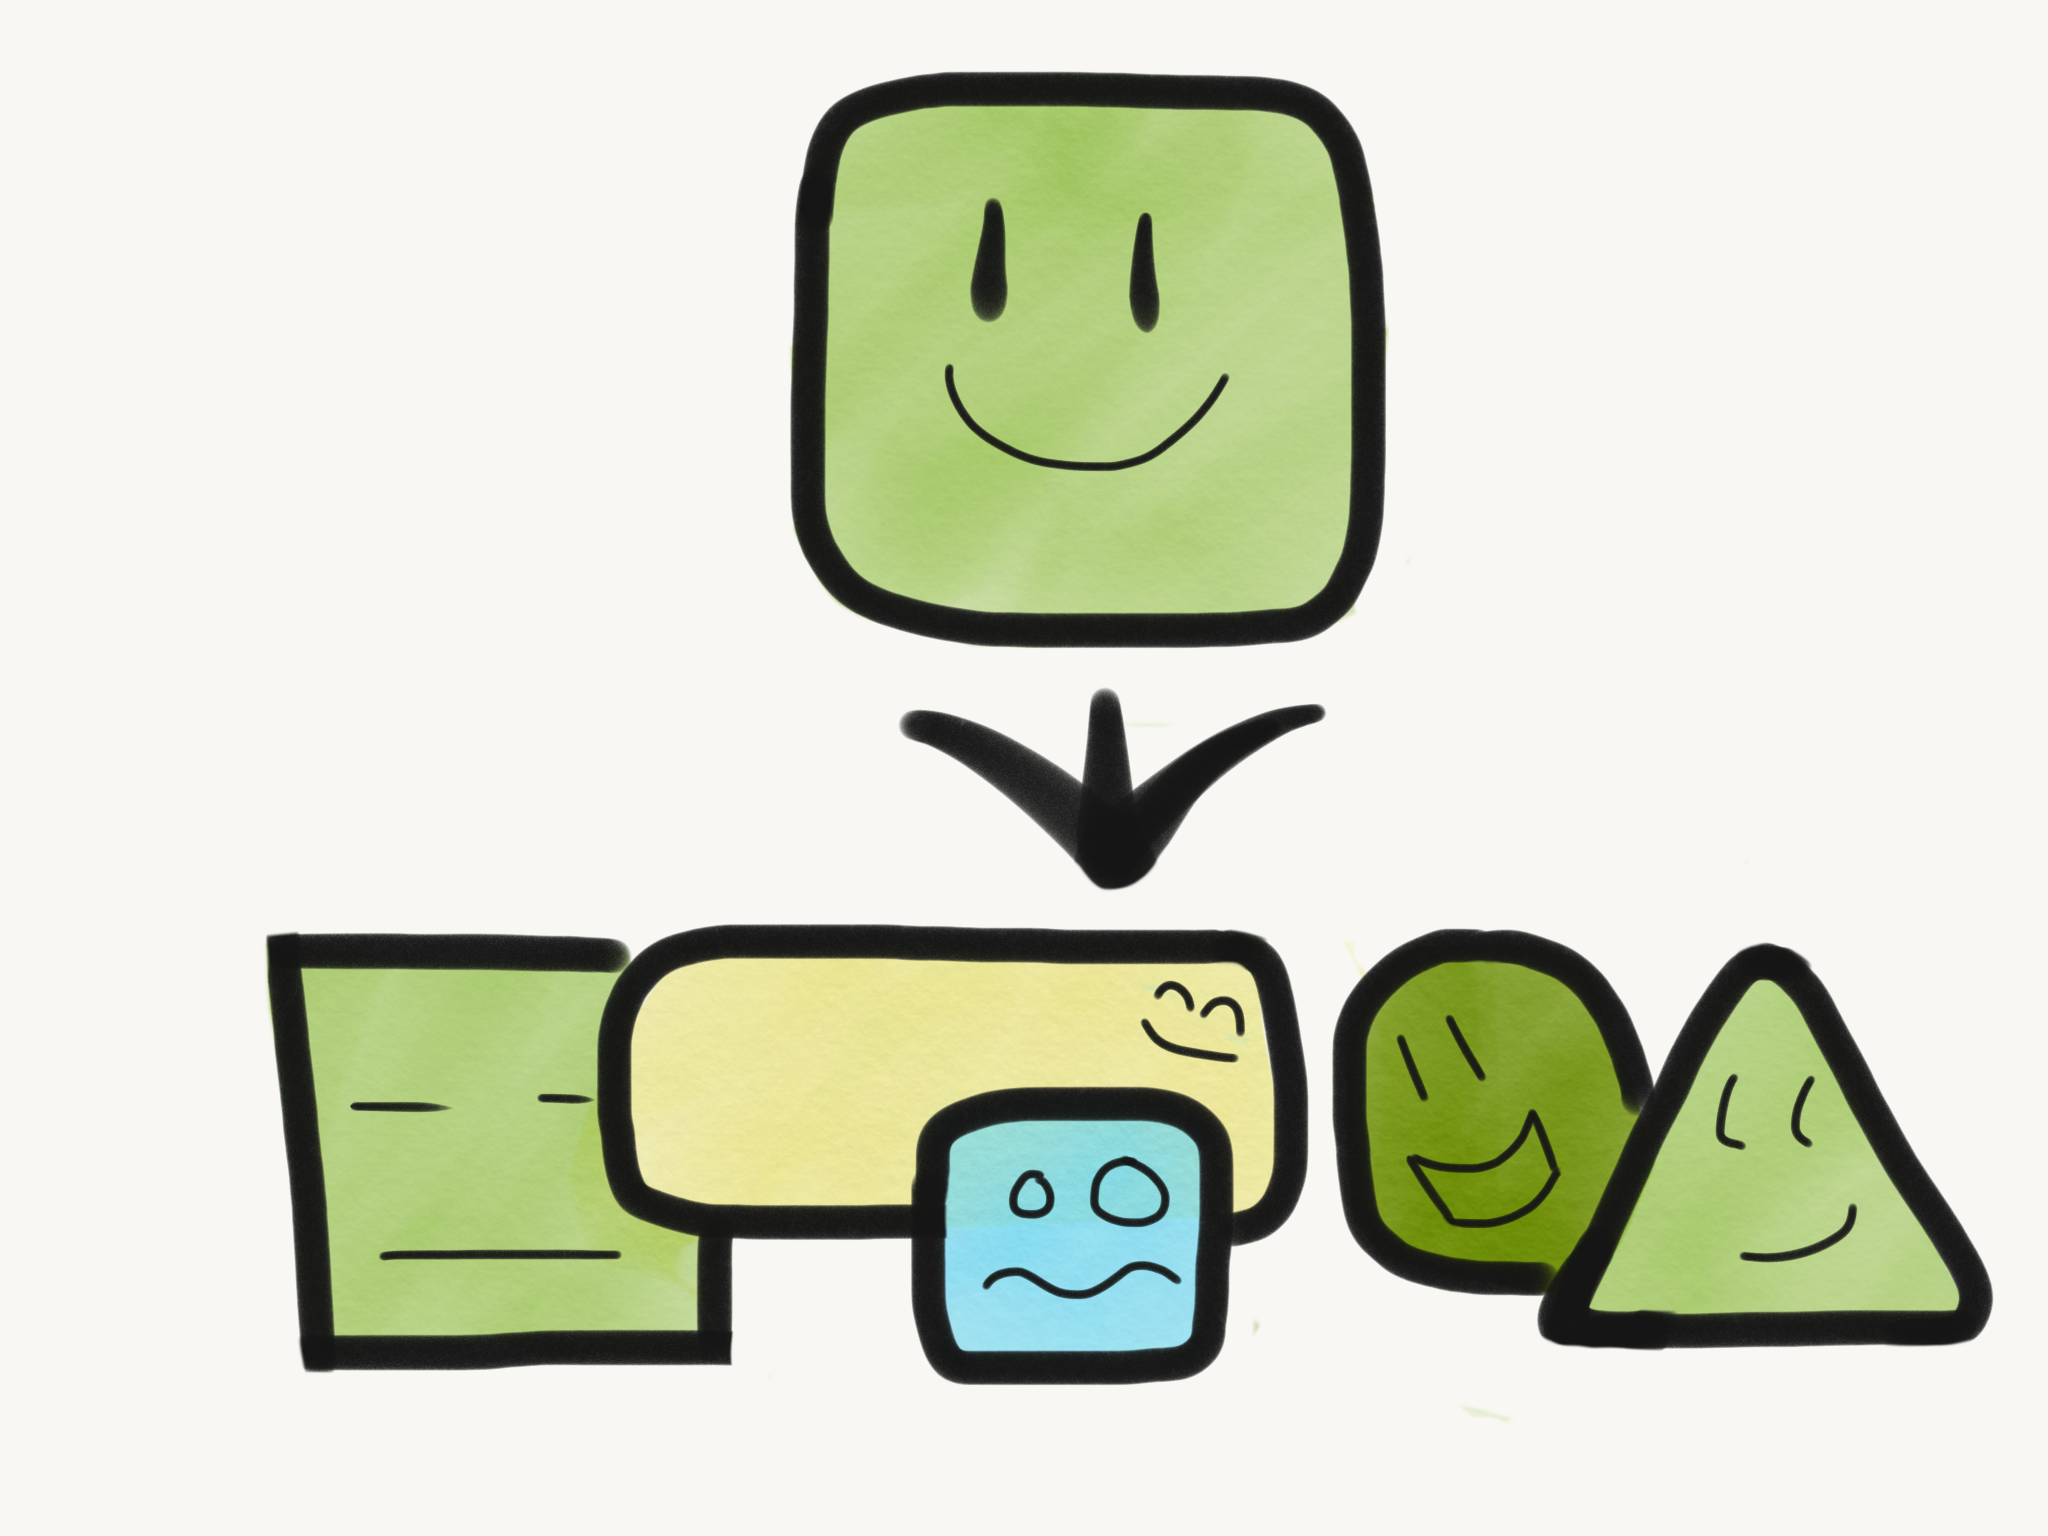
\includegraphics[width=\textwidth]{img/individual_evolvability.png}
        \caption{high individual evolvability}
        \label{subfig:canalization}
    \end{subfigure}%
    \hfill
    \begin{subfigure}[b]{0.5\textwidth}
        \centering
        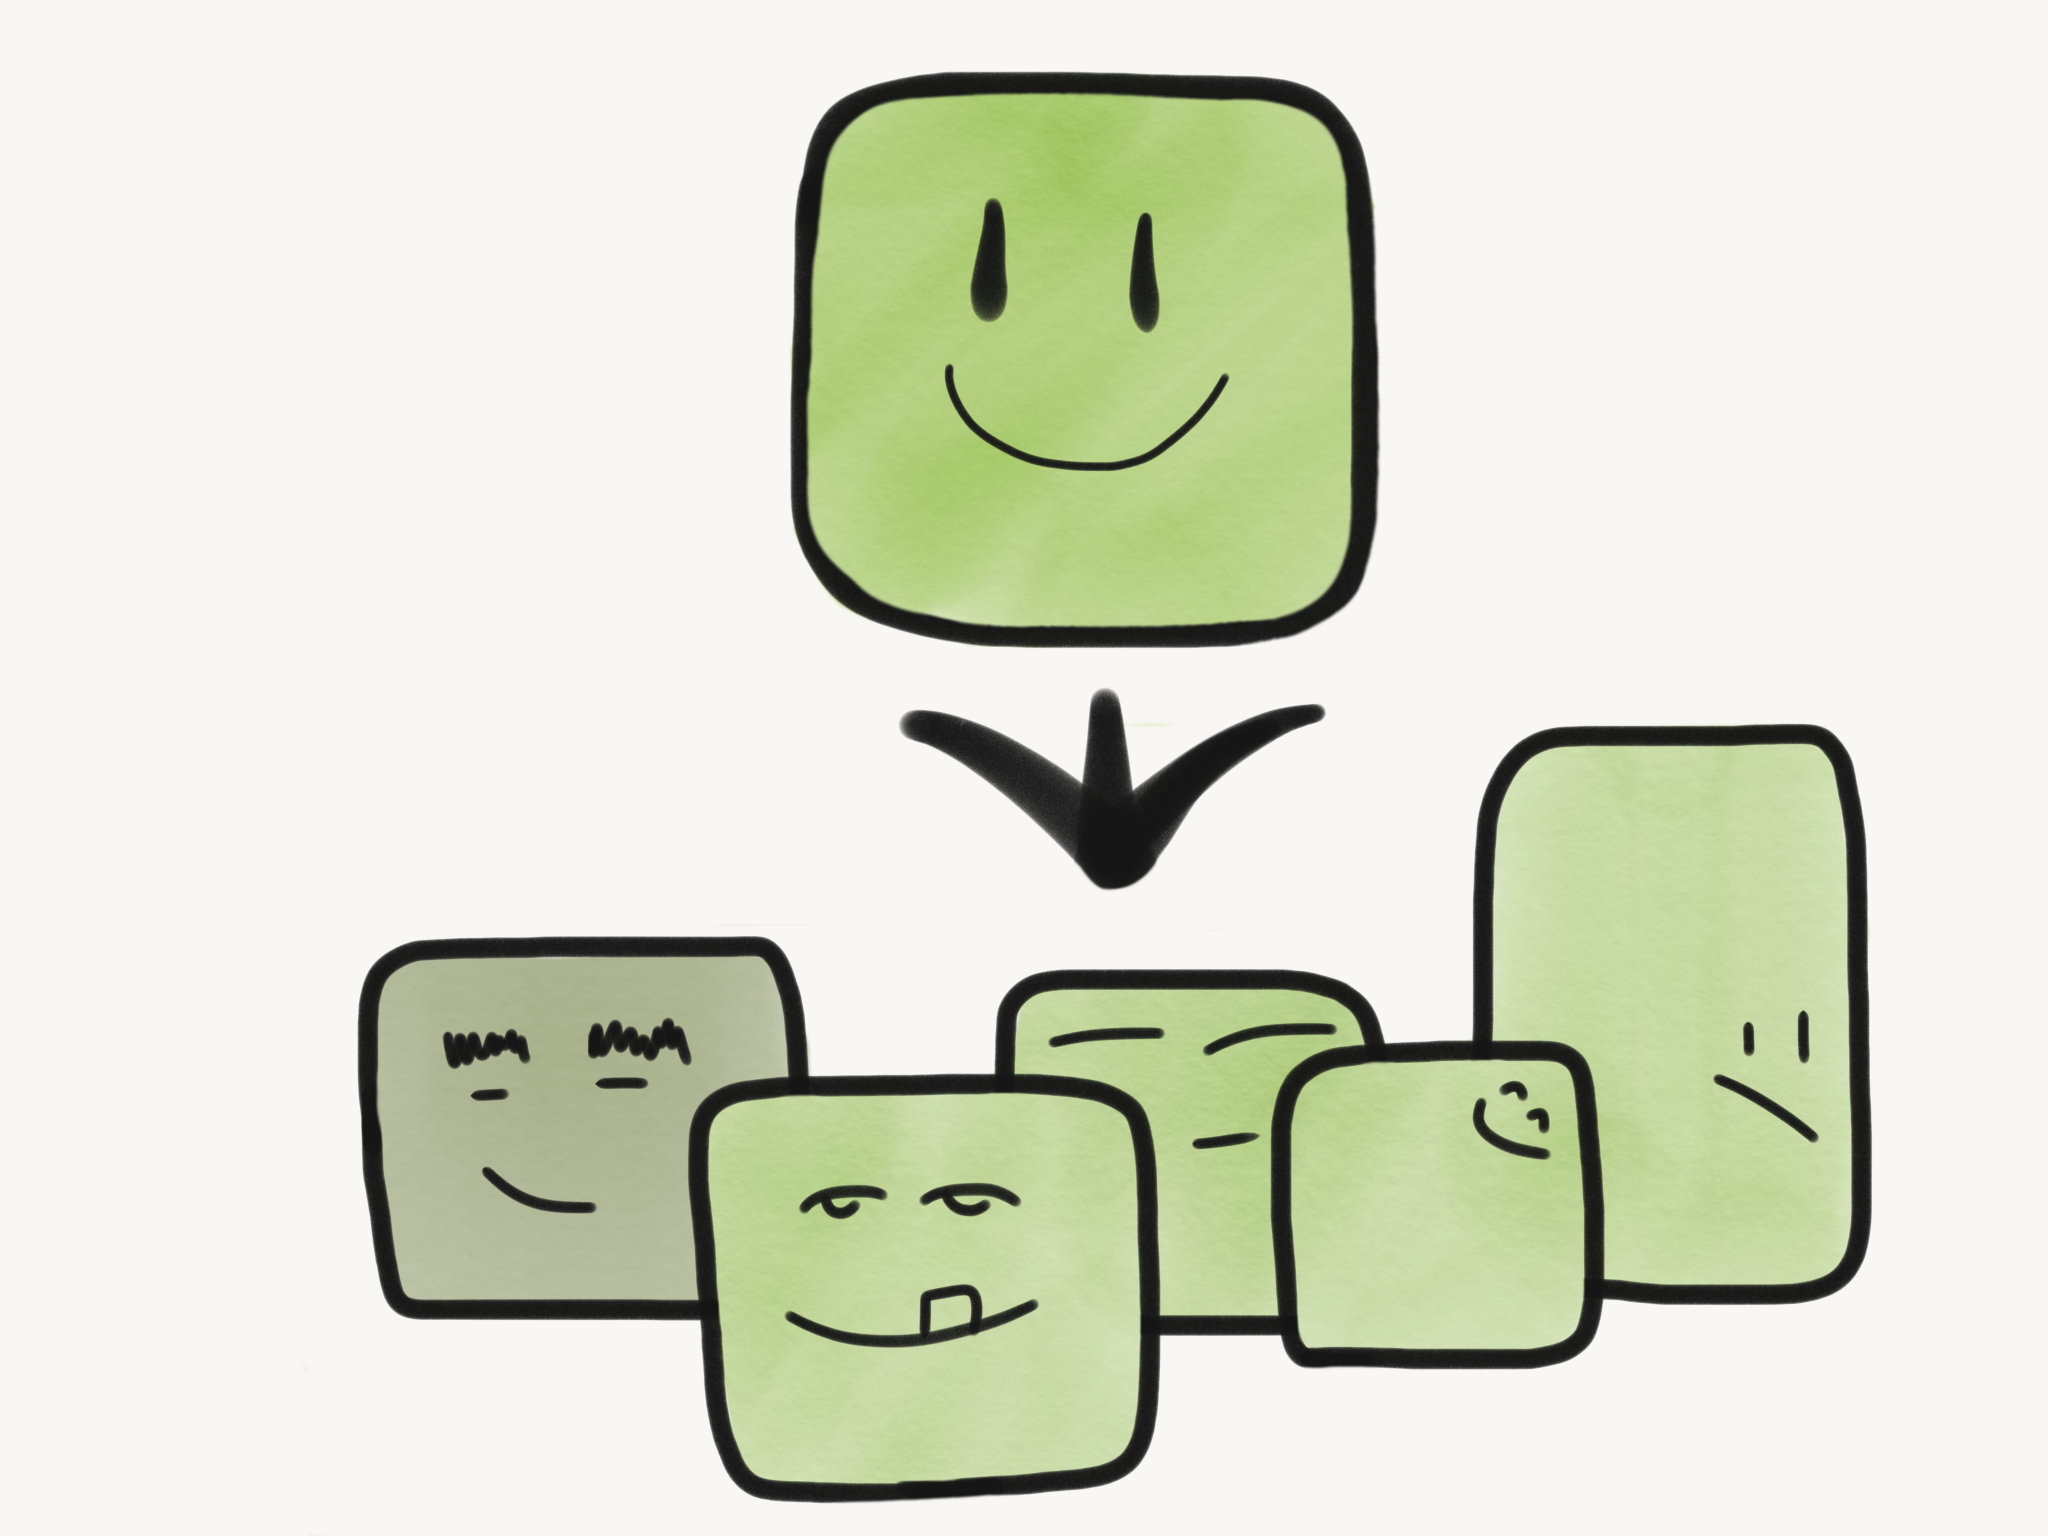
\includegraphics[width=\textwidth]{img/low_individual_evolvability.png}
        \caption{low individual evolvability}
        \label{subfig:no_canalization}
    \end{subfigure}
 	\captionsetup{singlelinecheck=off,justification=raggedright}
    \vspace{-4ex}
  \captionsetup{singlelinecheck=off,justification=raggedright}
  \caption{An illustration of individual evolvability, considering evolvability as heritable variation \cite{Wilder2015ReconcilingEvolvability}.}
  \label{fig:high_vs_low_individual_evolvability}
\end{figure}
\end{frame}

\subsection{Evolvability as Bias towards Useful Variation}

\begin{frame}{Evolvability as Bias towards Useful Variation}
  \begin{figure}
    \centering
    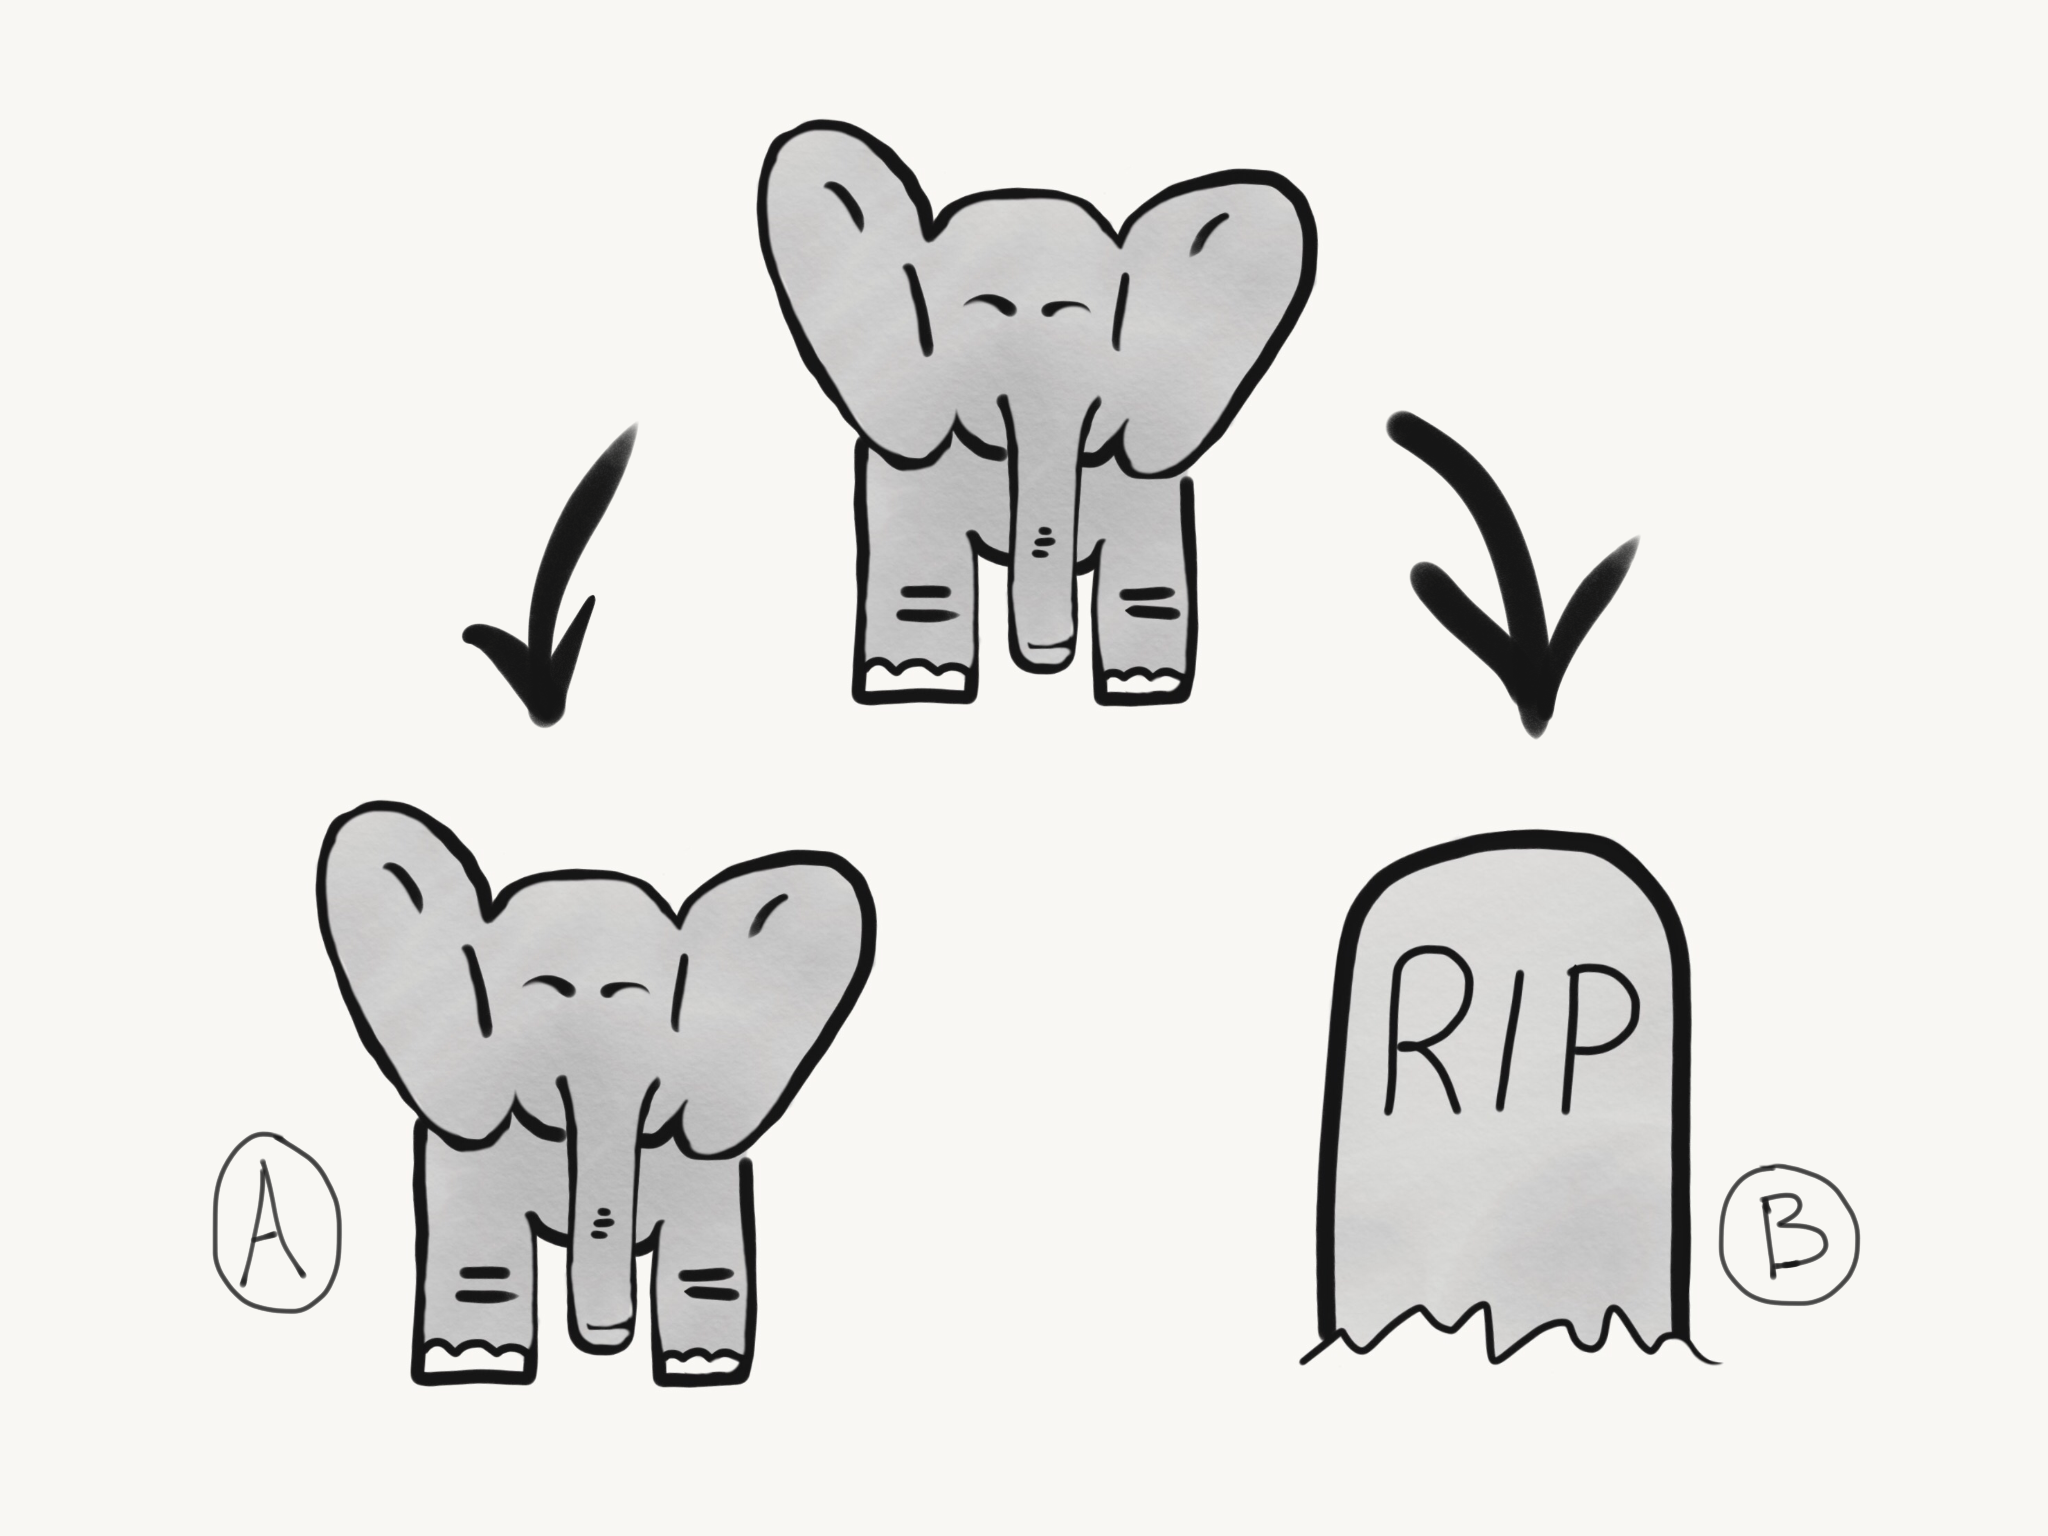
\includegraphics[width=0.8\textwidth]{img/robustness}
 	\captionsetup{singlelinecheck=off,justification=raggedright}
  	\caption{Illustration of robustness; high evolvability left and low evolvability right \cite{Downing2015IntelligenceSystems}.}
    \label{fig:robustness}
\end{figure}
\end{frame}

\begin{frame}{Motivation: Practical and Scientific Questions}
\begin{columns}
\begin{column}{0.6\textwidth}
\begin{figure}
  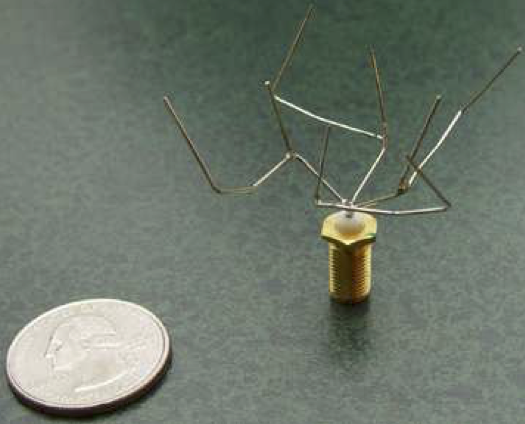
\includegraphics[width=\textwidth]{img/evolved_antenna} 
  \hspace{2ex}
  \caption{A spacecraft antenna design generated using evolutionary methods \cite[Figure 2(a)]{Hornby2006AutomatedAlgorithms}.}
  \label{fig:evolved_antenna}
\end{figure}
\end{column}
\begin{column}{0.4\textwidth}
\begin{center}
\begin{figure}
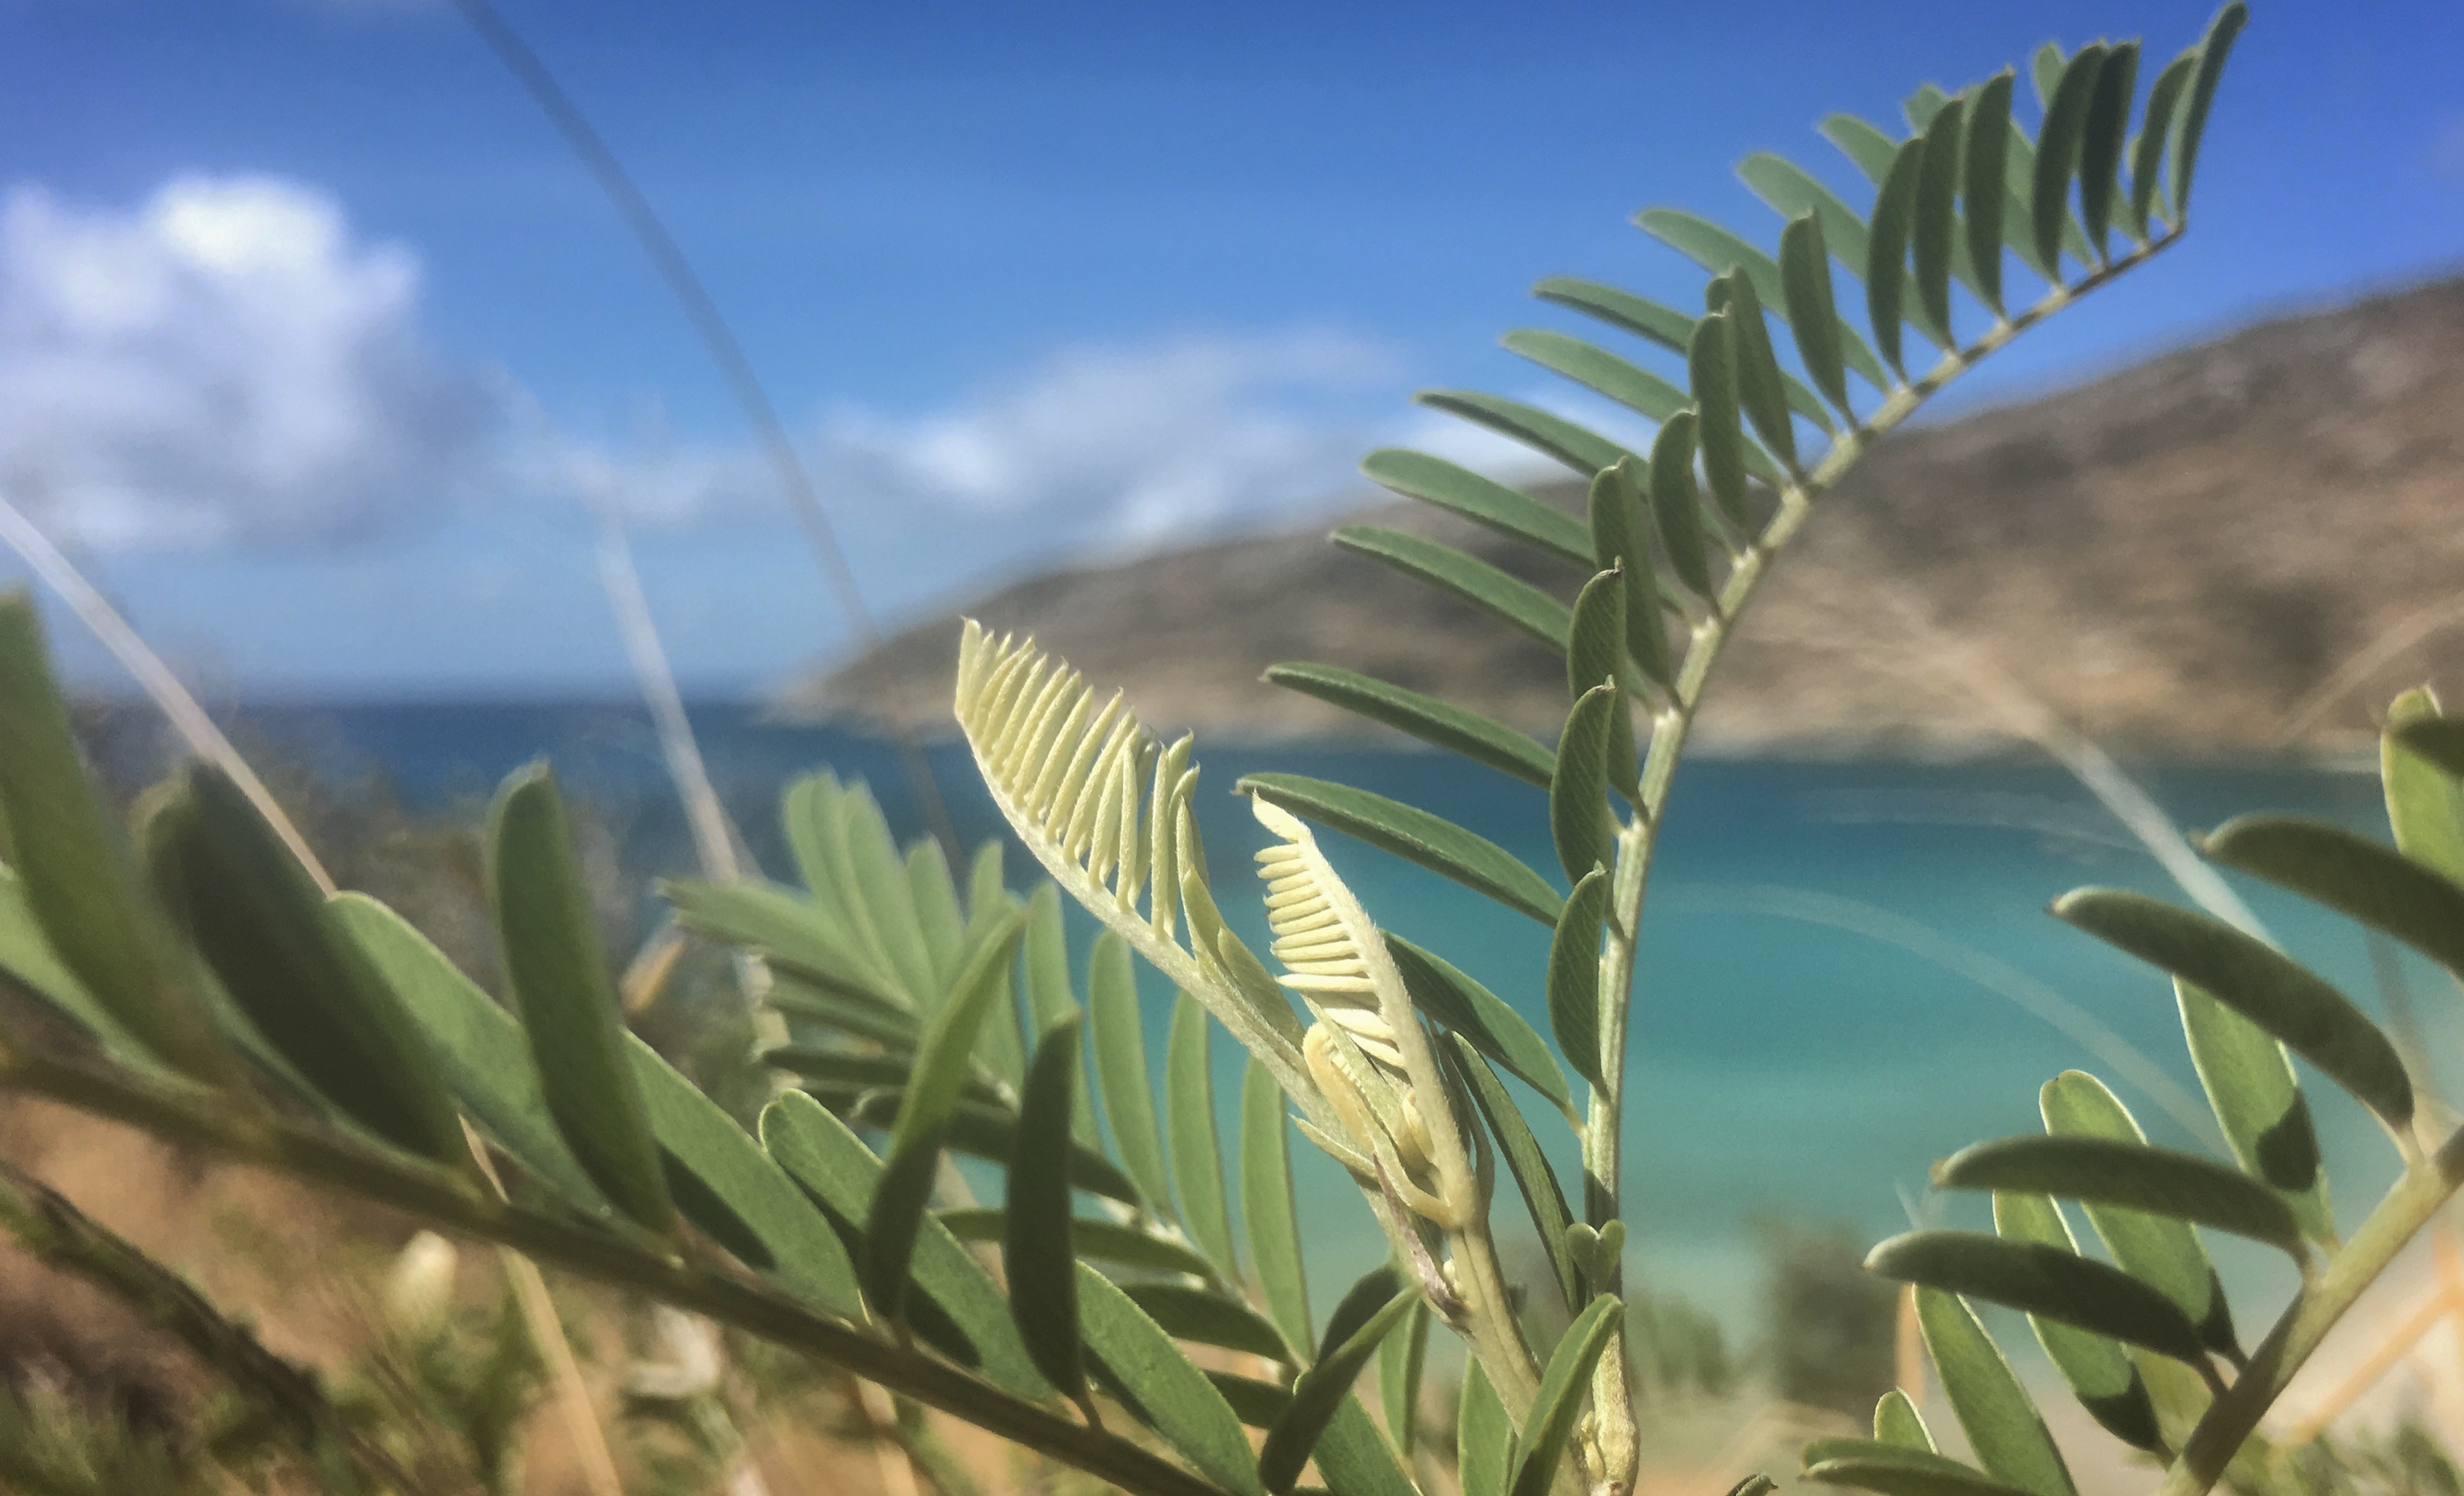
\includegraphics[width=\textwidth,trim={43cm 0 47cm 8cm},clip]{img/island_fern}
\caption{A biological frond design generated via evolution.}
\end{figure}
\end{center}
\end{column}
\end{columns}
\end{frame}

\section{Genetic Regulatory Network Model}

\begin{frame}{Model Framework}
\begin{columns}
\begin{column}{0.5\textwidth}
\begin{figure}
    \centering
    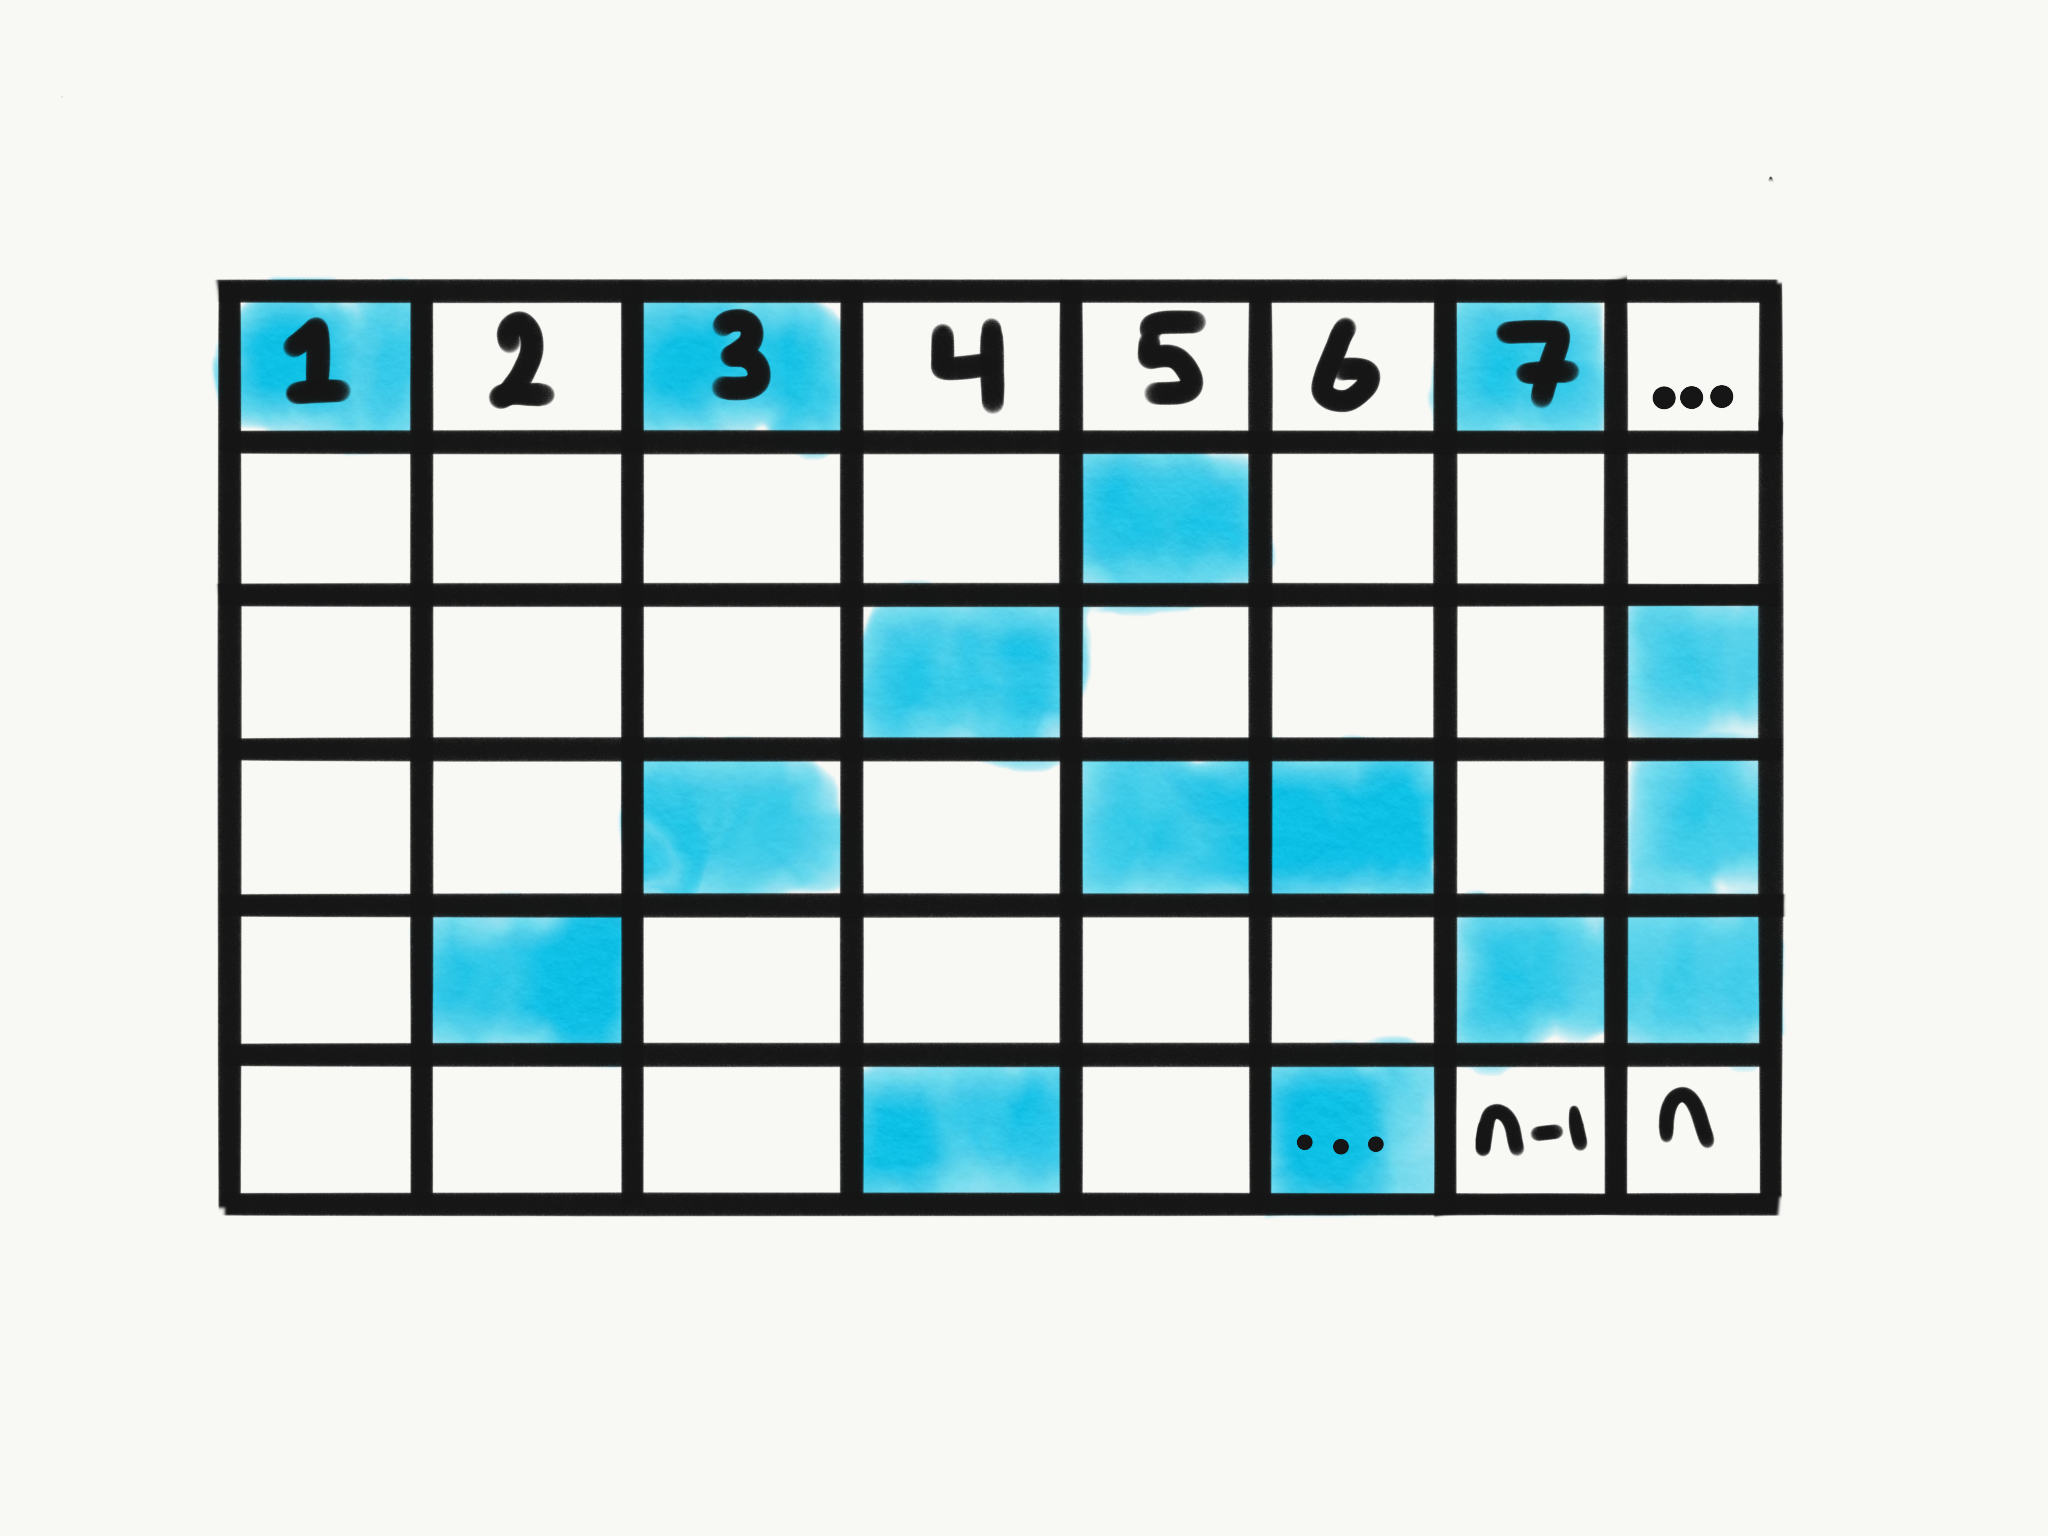
\includegraphics[width=\textwidth]{img/initial_state}
 	\captionsetup{singlelinecheck=off,justification=raggedright}
  	\caption{Chemical concentrations are represented as a list of boolean values.}
    \label{fig:initial_state}
\end{figure}
\end{column}

\begin{column}{0.5\textwidth}
\begin{figure}
    \centering
    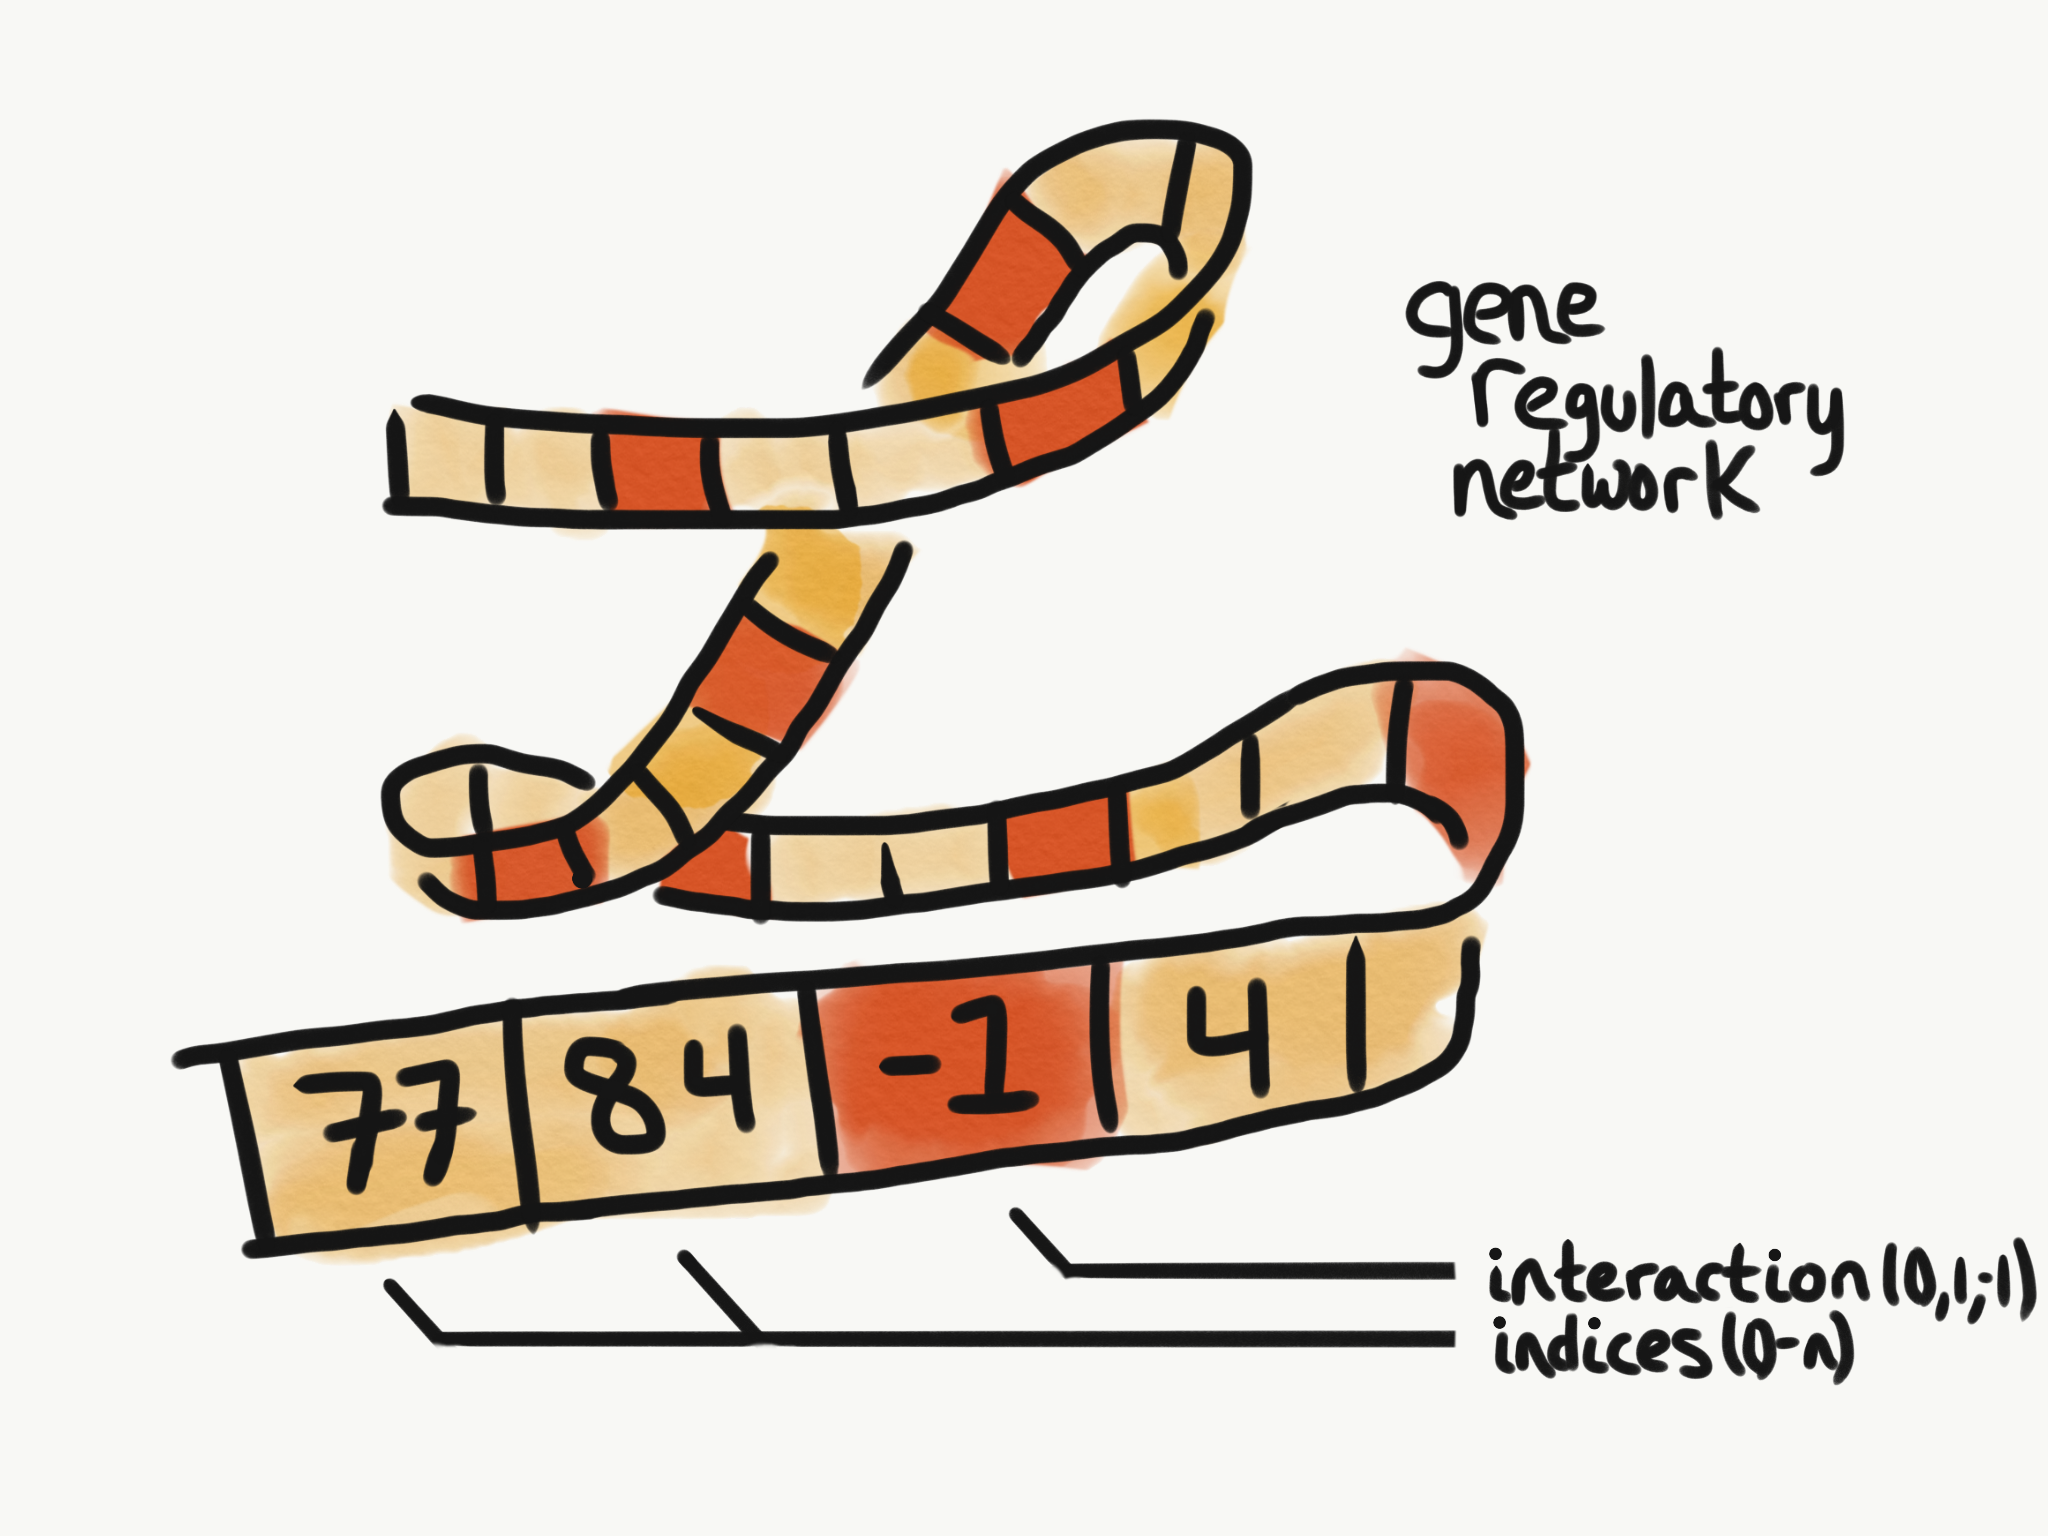
\includegraphics[width=\textwidth]{img/expanded_grn}
 	\captionsetup{singlelinecheck=off,justification=raggedright}
  	\caption{The GRN genotype is a set of if-then rules that acts on a set of chemical concentrations. The model employed was inspired by \cite{Wilder2015ReconcilingEvolvability}.}
    \label{fig:expanded_grn}
\end{figure}
\end{column}

\end{columns}
\end{frame}

\begin{frame}{Model Framework}
\begin{figure}
  \centering
  \begin{subfigure}[b]{\textwidth}
    \centering
    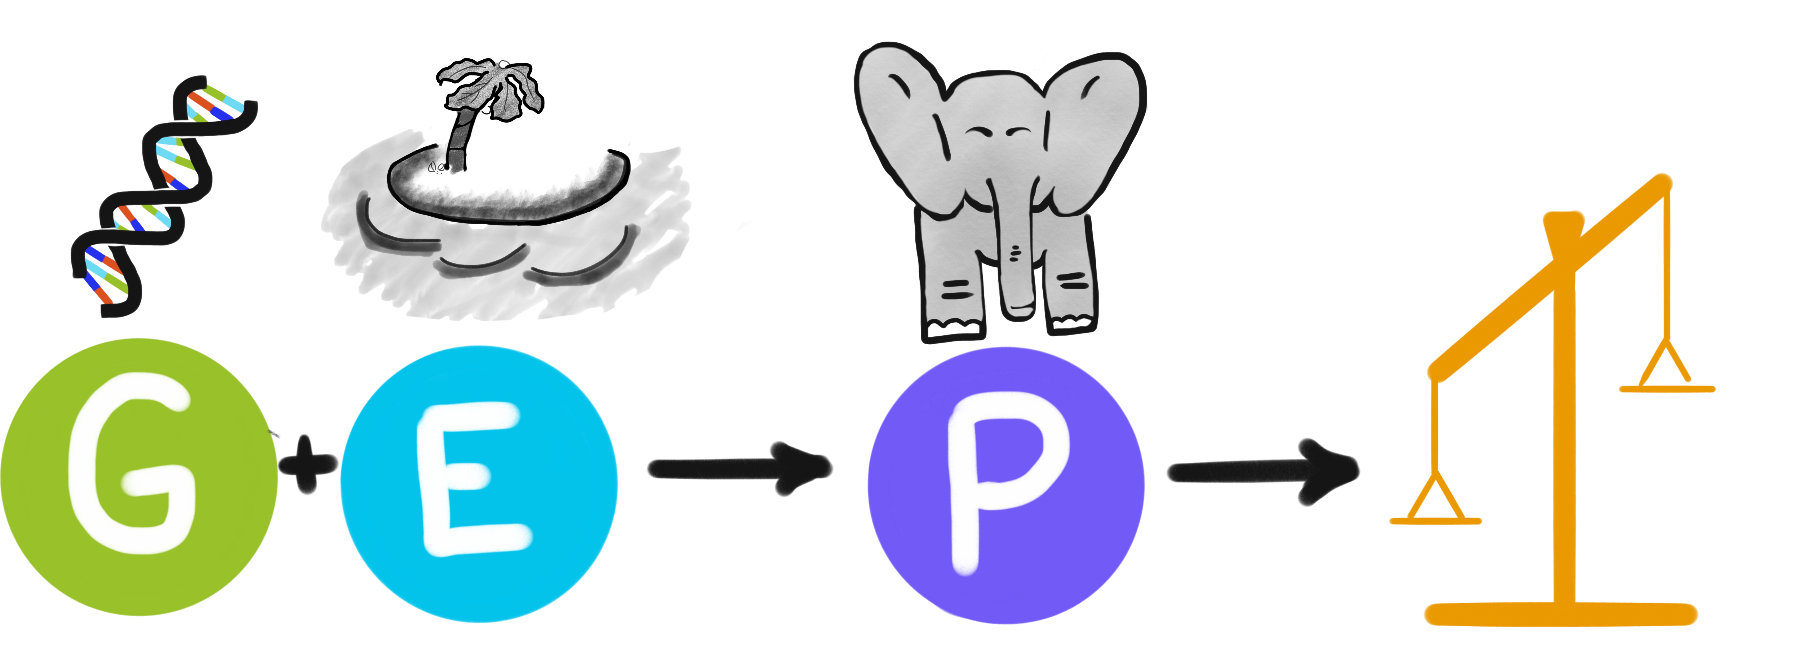
\includegraphics[width=0.6\textwidth]{img/bioscheme}
    \caption{biological inspiration}
    \label{subfig:bioscheme}
  \end{subfigure}
  \hfill
  \begin{subfigure}[b]{0.6\textwidth}
    \centering
    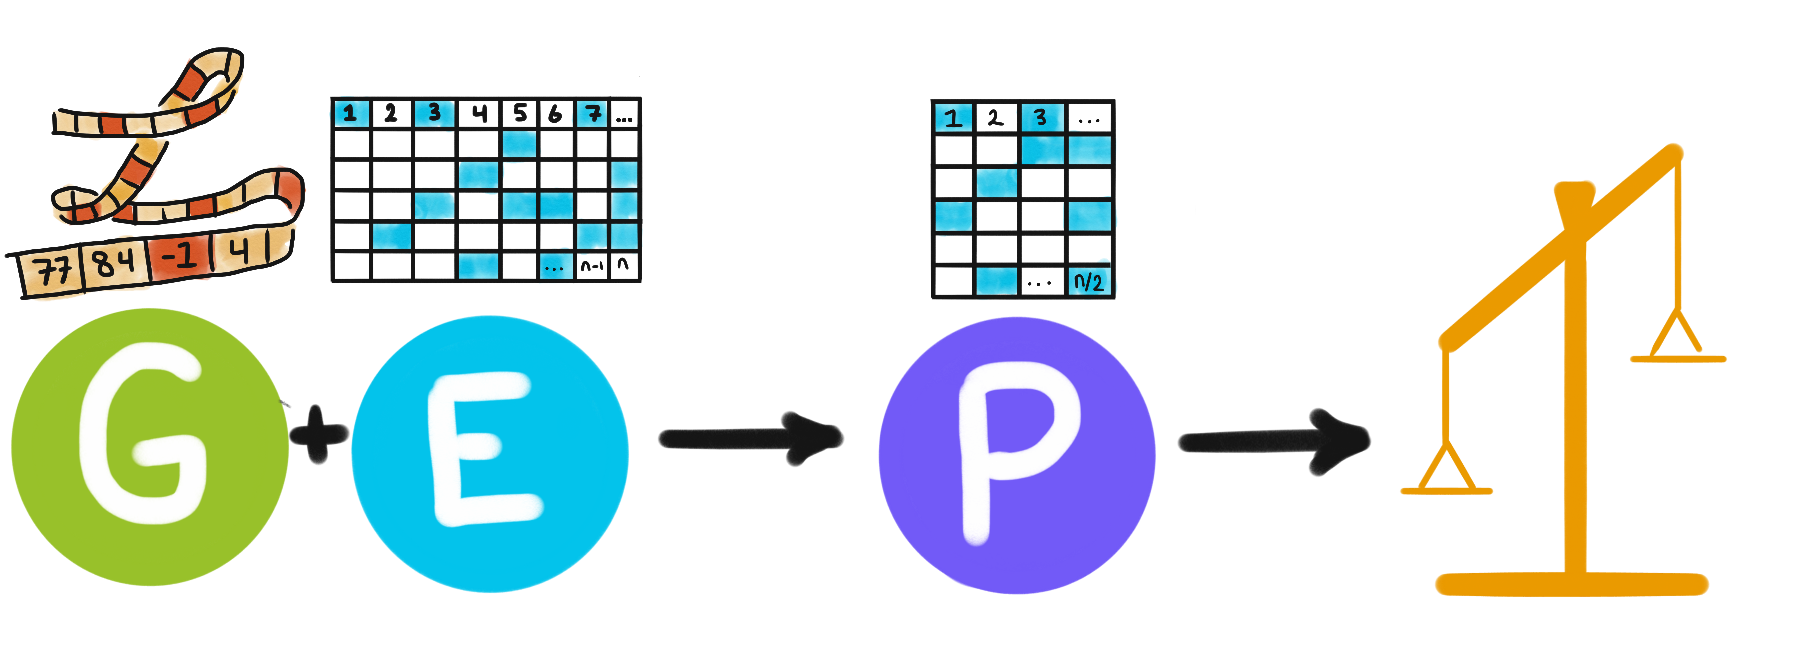
\includegraphics[width=\textwidth]{img/modelscheme}
    \caption{genetic regulatory network model}
     \label{subfig:modelscheme}
  \end{subfigure}
  \captionsetup{singlelinecheck=off,justification=raggedright}
  \caption{A comparison of the genetic regulatory network model and its biological inspiration.}
  \label{fig:model_bio_comparison}
\end{figure}
\end{frame}






\section{Experiment: Direct Plasticity}


\begin{frame}{Direct Plasticity: Initial State Perturbation}
\begin{figure}
  \centering
  \begin{subfigure}[b]{\textwidth}
    \centering
    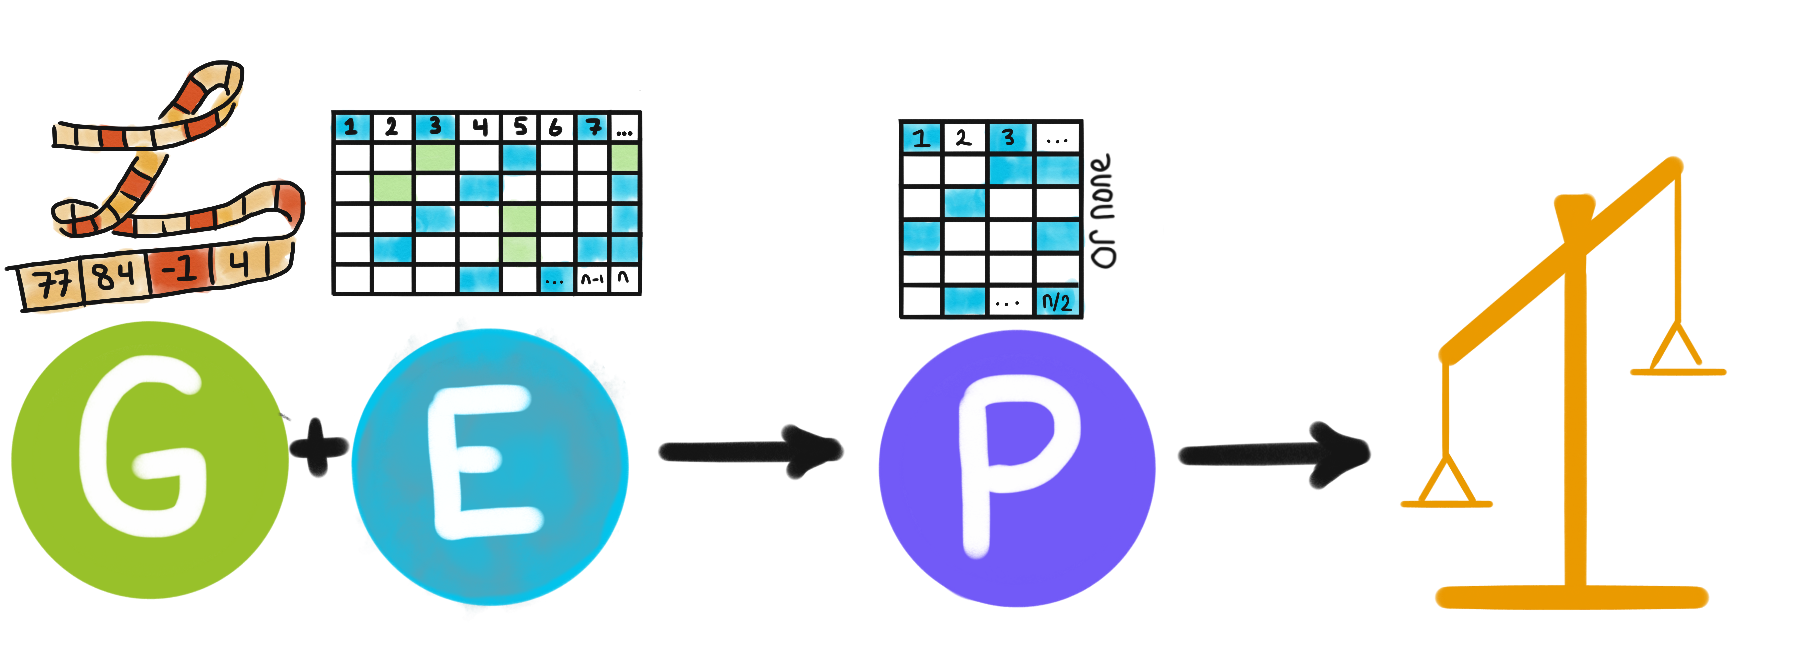
\includegraphics[width=0.6\textwidth]{img/directscheme}
    \caption{experimental scheme}
    \label{subfig:directscheme}
  \end{subfigure}
  \hfill
  \begin{subfigure}[b]{0.6\textwidth}
    \centering
    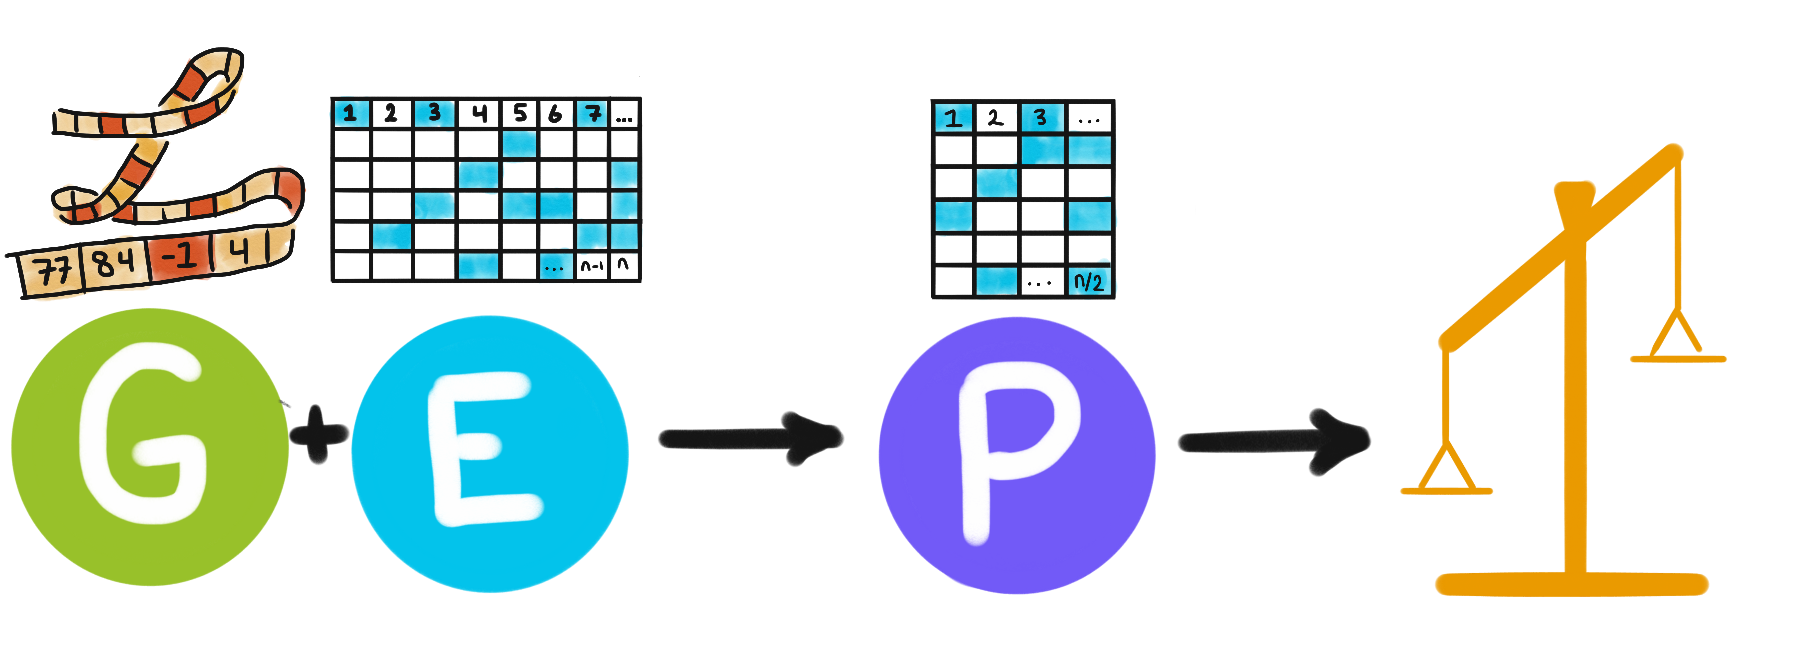
\includegraphics[width=\textwidth]{img/modelscheme}
    \caption{control scheme}
     \label{subfig:controlscheme}
  \end{subfigure}
  \captionsetup{singlelinecheck=off,justification=raggedright}
  \caption{A comparison of the control and experimental schemes employed to investigate the relationship between direct plasticity and evolvability.}
  \label{fig:direct_plasticity_scheme}
\end{figure}
\end{frame}

\begin{frame}{Mutational Outcome Frequencies}
\begin{figure}
    \centering
    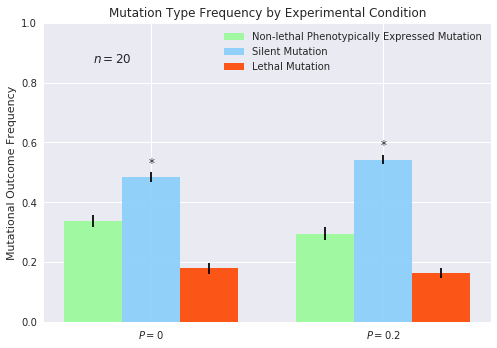
\includegraphics[width=0.8\textwidth]{img/mutation_type_direct}
 	\captionsetup{singlelinecheck=off,justification=raggedright}
  	\caption{Comparison of mutational outcome frequencies for champions evolved with and without initial state perturbation.}
    \label{fig:mutation_type_indirect}
\end{figure}
\end{frame}

\begin{frame}{Direct Plasticity Results: Summary}
\begin{itemize}
  \item direct plasticity increases robustness to mutation
  \item as in \cite{Reisinger2005TowardsEvolvability}, repeated evaluations ($n=10$) were required to observe impact of direct plasticity
\end{itemize}
\end{frame}

\section{Experiment: Indirect Plasticity}

\begin{frame}{Indirect Plasticity: Conditional Initial State}
\begin{figure}
  \centering
  \begin{subfigure}[b]{0.5\textwidth}
    \centering
    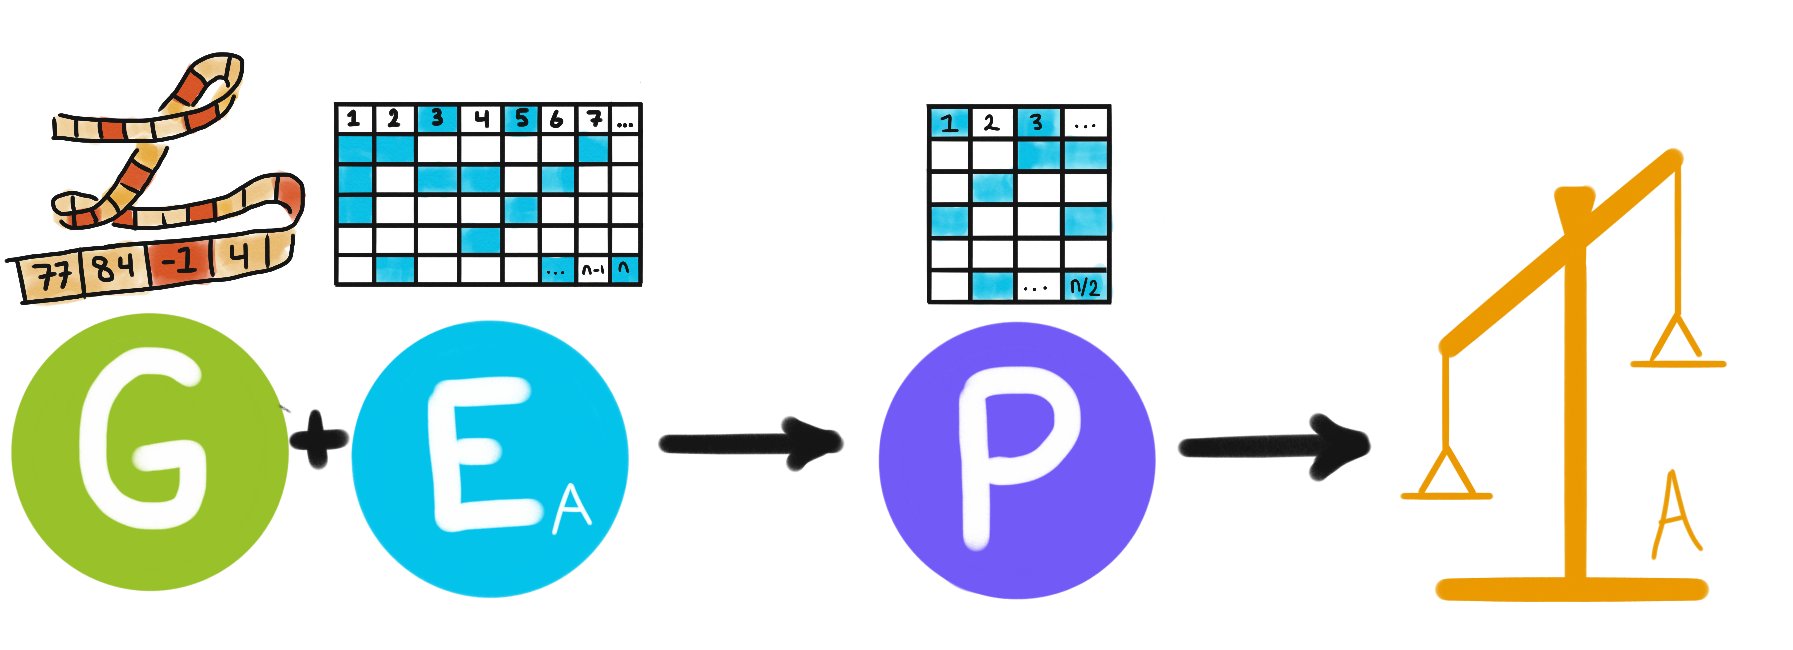
\includegraphics[width=\textwidth]{img/indirectschemeA} \\
    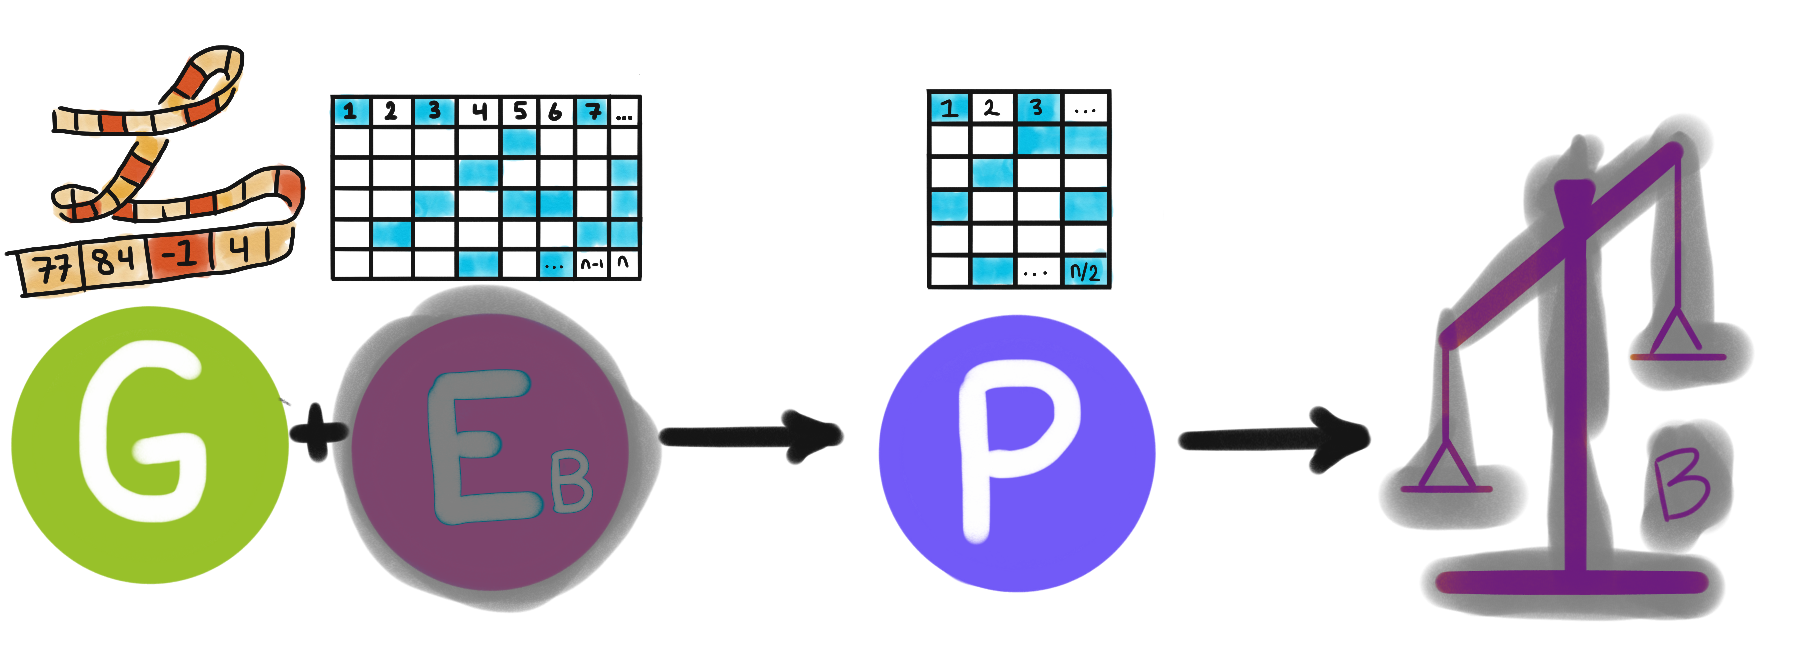
\includegraphics[width=\textwidth]{img/indirectschemeB}
    \caption{experimental scheme}
    \label{subfig:directscheme}
  \end{subfigure}%
  \hfill
  \begin{subfigure}[b]{0.5\textwidth}
    \centering
    
 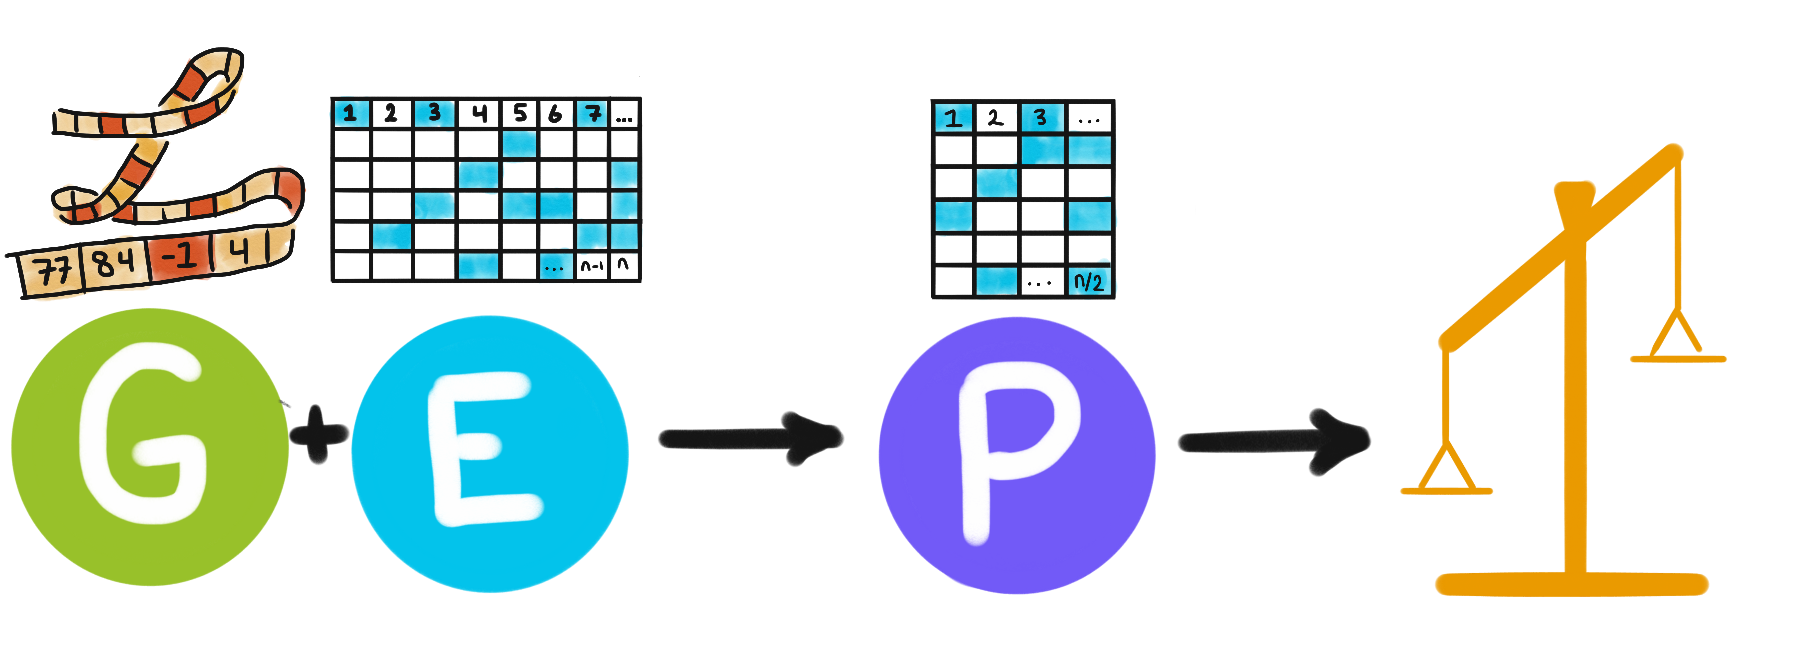
\includegraphics[width=\textwidth]{img/modelscheme} \\
 \vspace{5ex}
    
    \caption{control scheme}
     \label{subfig:controlscheme}
  \end{subfigure}
  \captionsetup{singlelinecheck=off,justification=raggedright}
  \caption{A comparison of the control and experimental schemes employed to investigate the relationship between indirect plasticity and evolvability.}
  \label{fig:direct_plasticity_scheme}
\end{figure}
\end{frame}

\begin{frame}{Evidence for Indirect Plasticity}
\begin{figure}
    \centering
    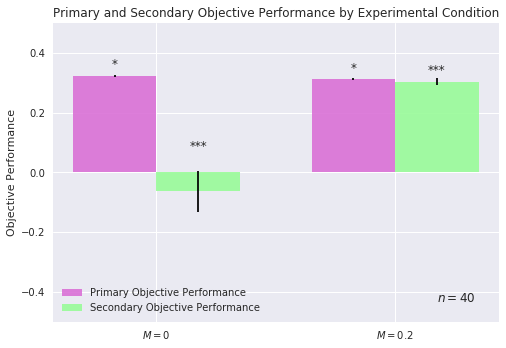
\includegraphics[width=0.8\textwidth]{img/primary_secondary_performance}
 	\captionsetup{singlelinecheck=off,justification=raggedright}
  	\caption{Comparison of objective performances of champions evolved with only primary condition/objective pair versus with both primary and secondary condition/objective pairs.}
    \label{fig:ev_w0}
\end{figure}
\end{frame}

\begin{frame}{Mutational Outcome Frequencies}
\begin{figure}
    \centering
    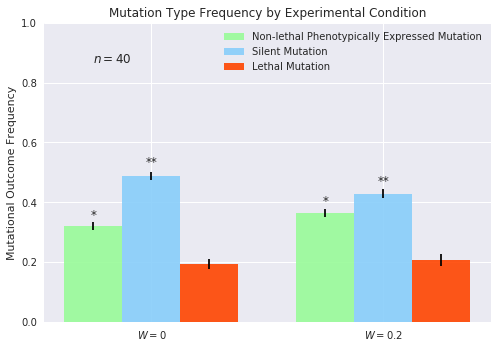
\includegraphics[width=0.8\textwidth]{img/mutation_type_indirect}
 	\captionsetup{singlelinecheck=off,justification=raggedright}
  	\caption{Comparison of mutational outcome frequencies for champions evolved with only primary condition/objective pair versus with both primary and secondary condition/objective pairs.}
    \label{fig:mutation_type_indirect}
\end{figure}
\end{frame}


\begin{frame}{Indirect Plasticity Results: Summary}
\begin{itemize}
  \item indirect plasticity observed
  \item indirect plasticity increases sensitivity to mutation
\end{itemize}
\end{frame}

\section{Experiment: Combined Plasticity}

\begin{frame}{Combined Plasticity: Conditional Initial State with Perturbation}
\begin{figure}
  \centering
  \begin{subfigure}[b]{0.5\textwidth}
    \centering
    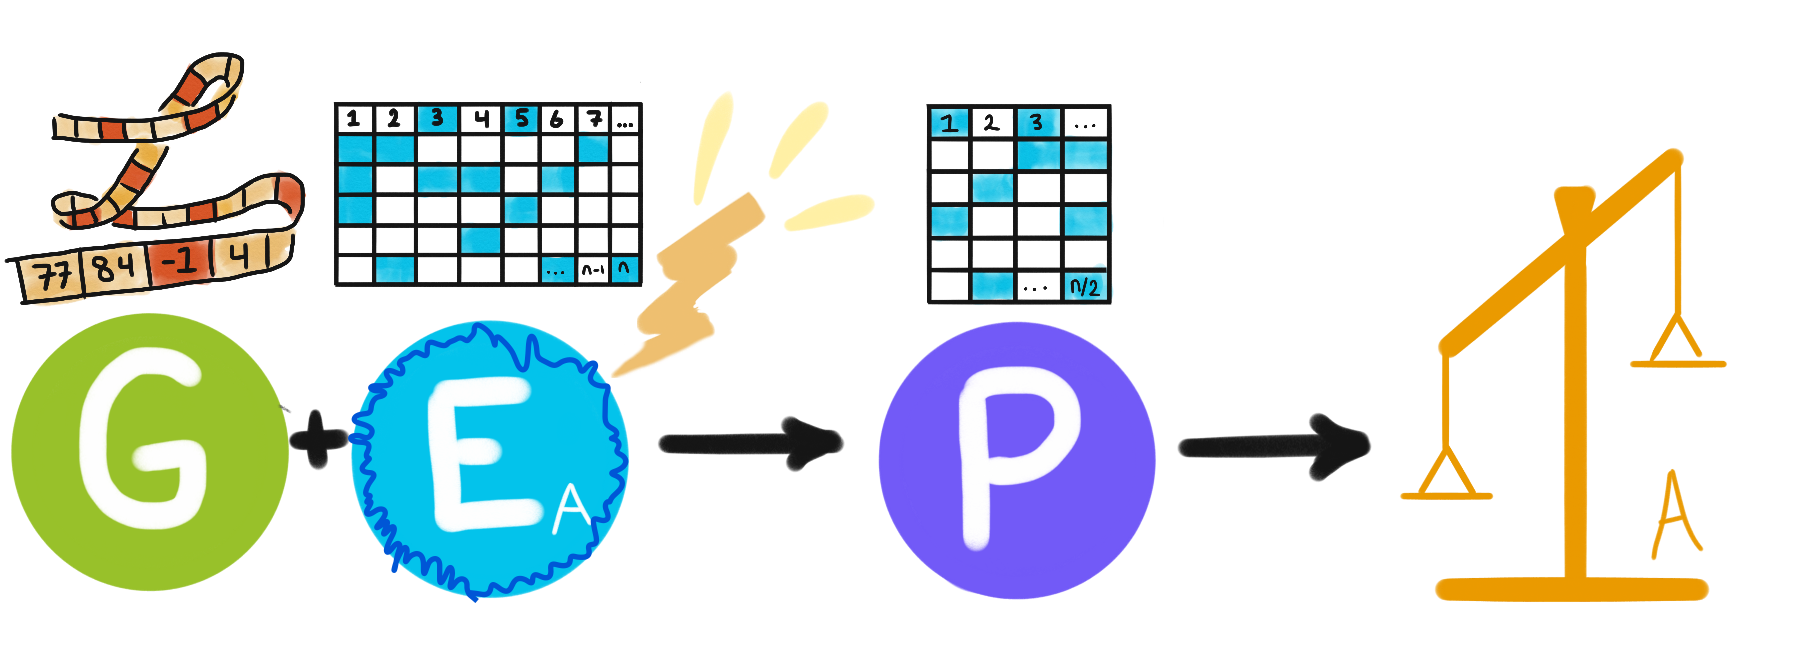
\includegraphics[width=\textwidth]{img/combinedschemeA} \\
    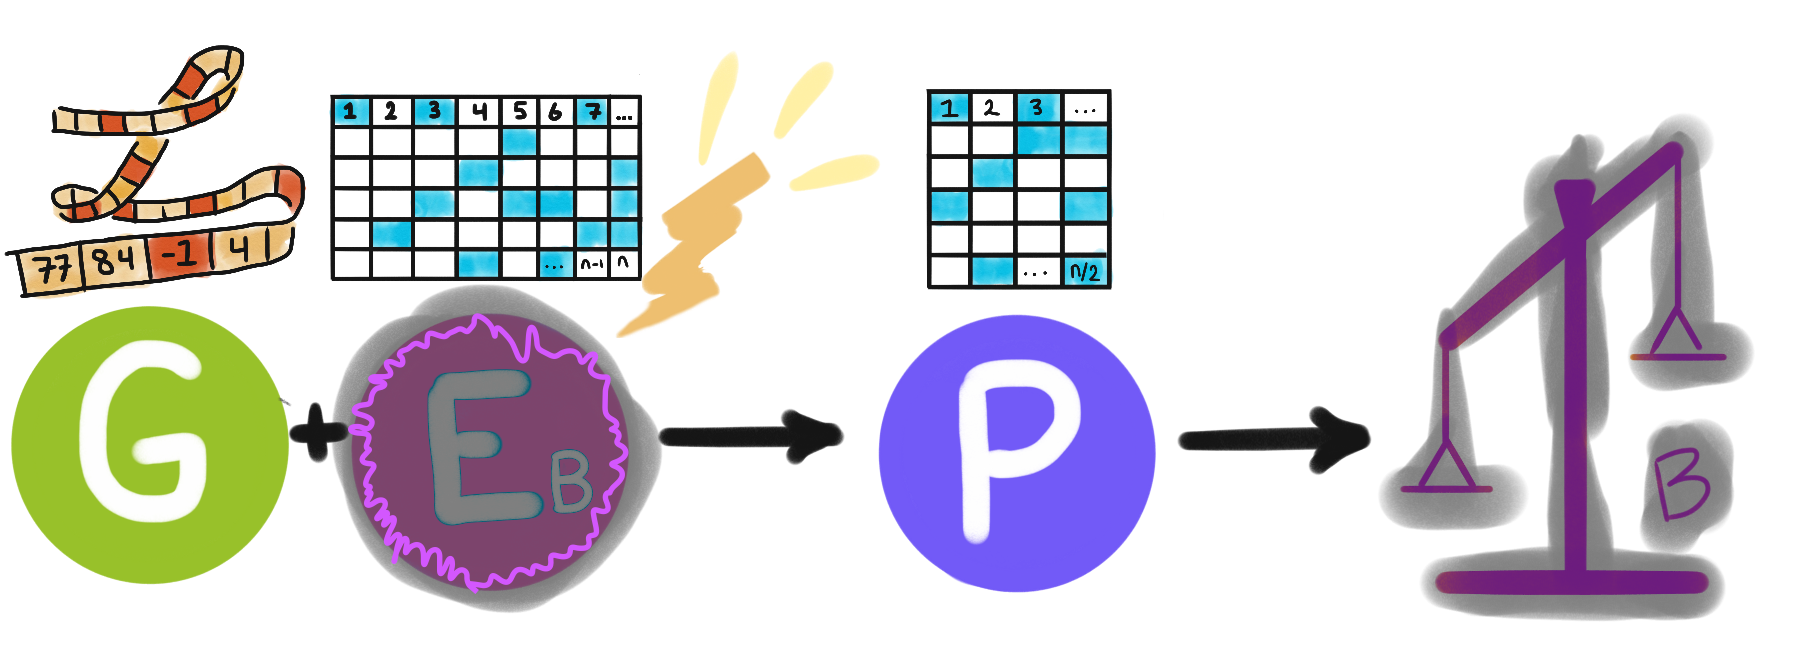
\includegraphics[width=\textwidth]{img/combinedschemeB}
    \caption{experimental scheme}
    \label{subfig:directscheme}
  \end{subfigure}%
  \hfill
  \begin{subfigure}[b]{0.5\textwidth}
    \centering
    
    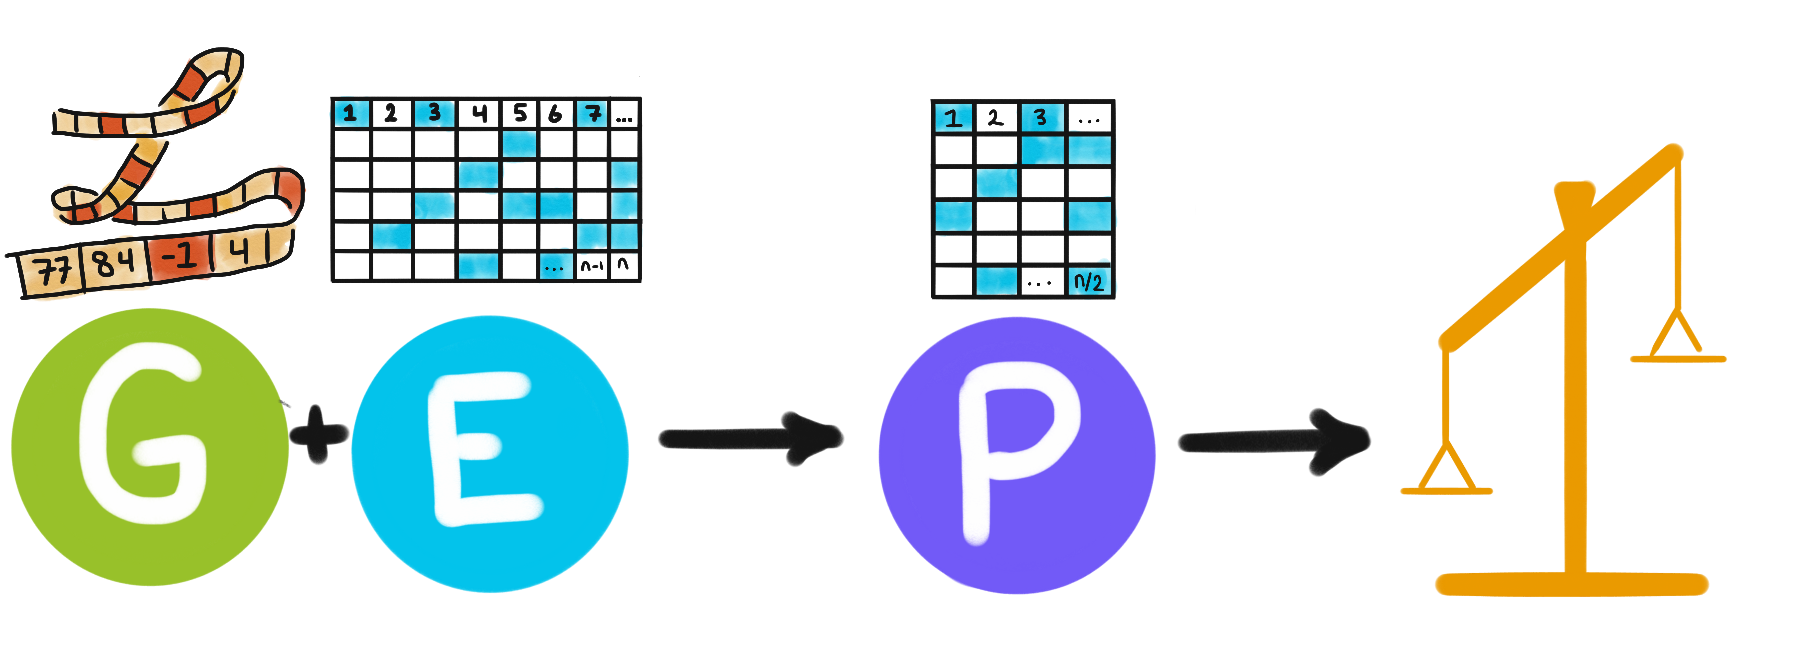
\includegraphics[width=\textwidth]{img/modelscheme} \\
 \vspace{5ex}
    \caption{control scheme}
     \label{subfig:controlscheme}
  \end{subfigure}
  \captionsetup{singlelinecheck=off,justification=raggedright}
  \caption{A comparison of the control and experimental schemes employed to investigate the relationship between combined plasticity and evolvability.}
  \label{fig:combined_plasticity_scheme}
\end{figure}
\end{frame}


% \section{Closing Thoughts}

\begin{frame}{Next Steps}
\begin{columns}
\begin{column}{0.6\textwidth}
\begin{itemize}
\item investigate structural changes in gene regulatory networks induced by plasticity
\item investigate interaction of direct and indirect plasticity
\item attempt to demonstrate situation where search with plasticity outperforms search without
\end{itemize}
\end{column}
\begin{column}{0.4\textwidth}
\begin{center}
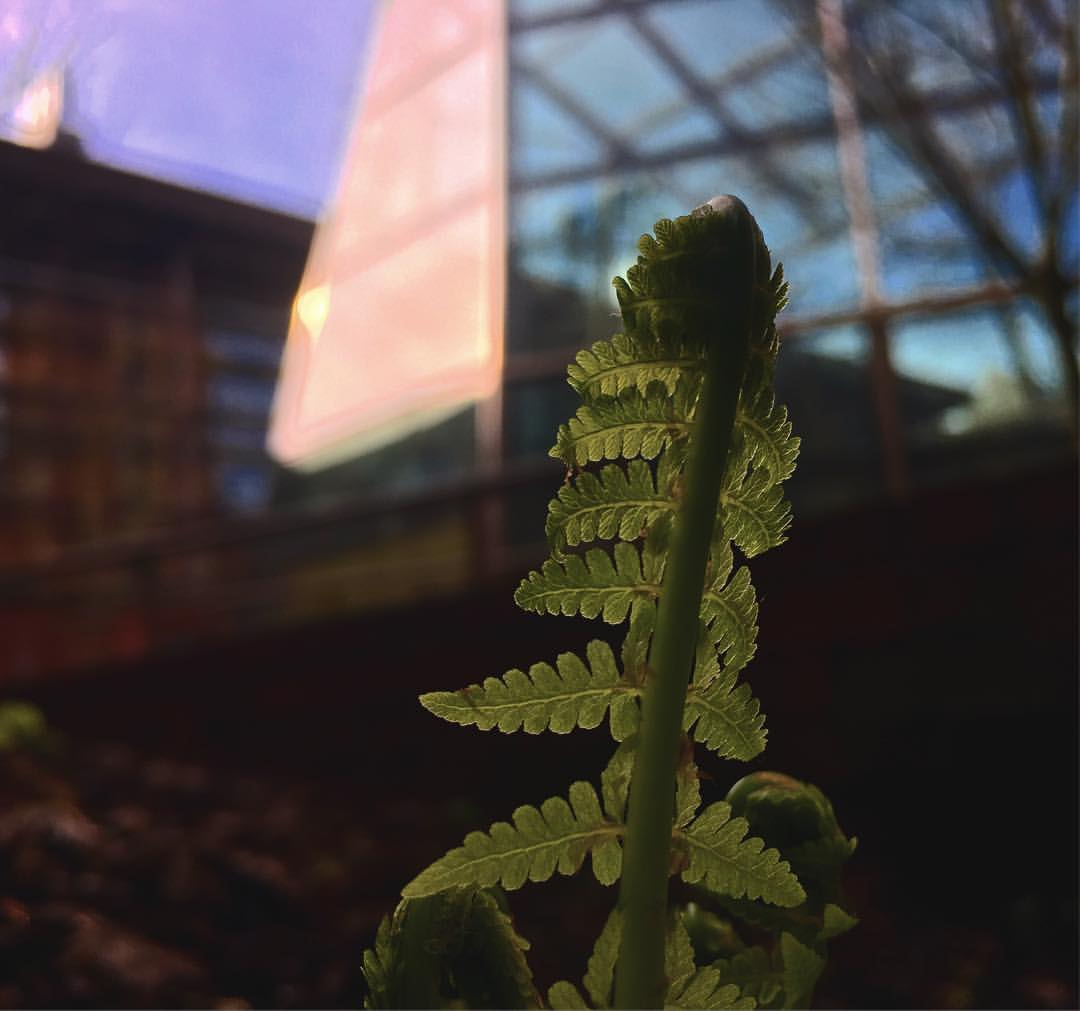
\includegraphics[width=\textwidth,trim={7cm 0 8cm 0},clip]{img/oppfern}
\end{center}
\end{column}
\end{columns}
\end{frame}

\begin{frame}{Closing Thoughts: Practical Applications}
\begin{figure}
  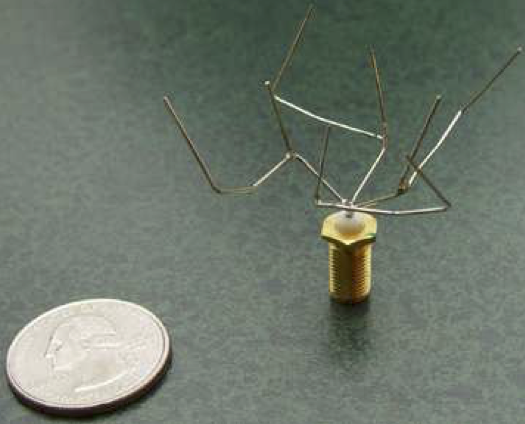
\includegraphics[width=\textwidth]{img/evolved_antenna} 
  \hspace{2ex}
  \caption{A spacecraft antenna design generated using evolutionary methods \cite[Figure 2(a)]{Hornby2006AutomatedAlgorithms}.}
  \label{fig:evolved_antenna}
\end{figure}
\end{frame}

\begin{frame}{Closign Thoughts: Scientific Questions}
\begin{columns}
\begin{column}{0.6\textwidth}
\begin{itemize}
\item at what level of abstraction can the power of biological evolution be harnessed in a computational model?
\item what are the fundamental mechanisms at play in evolution?
\end{itemize}
\end{column}
\begin{column}{0.4\textwidth}
\begin{center}
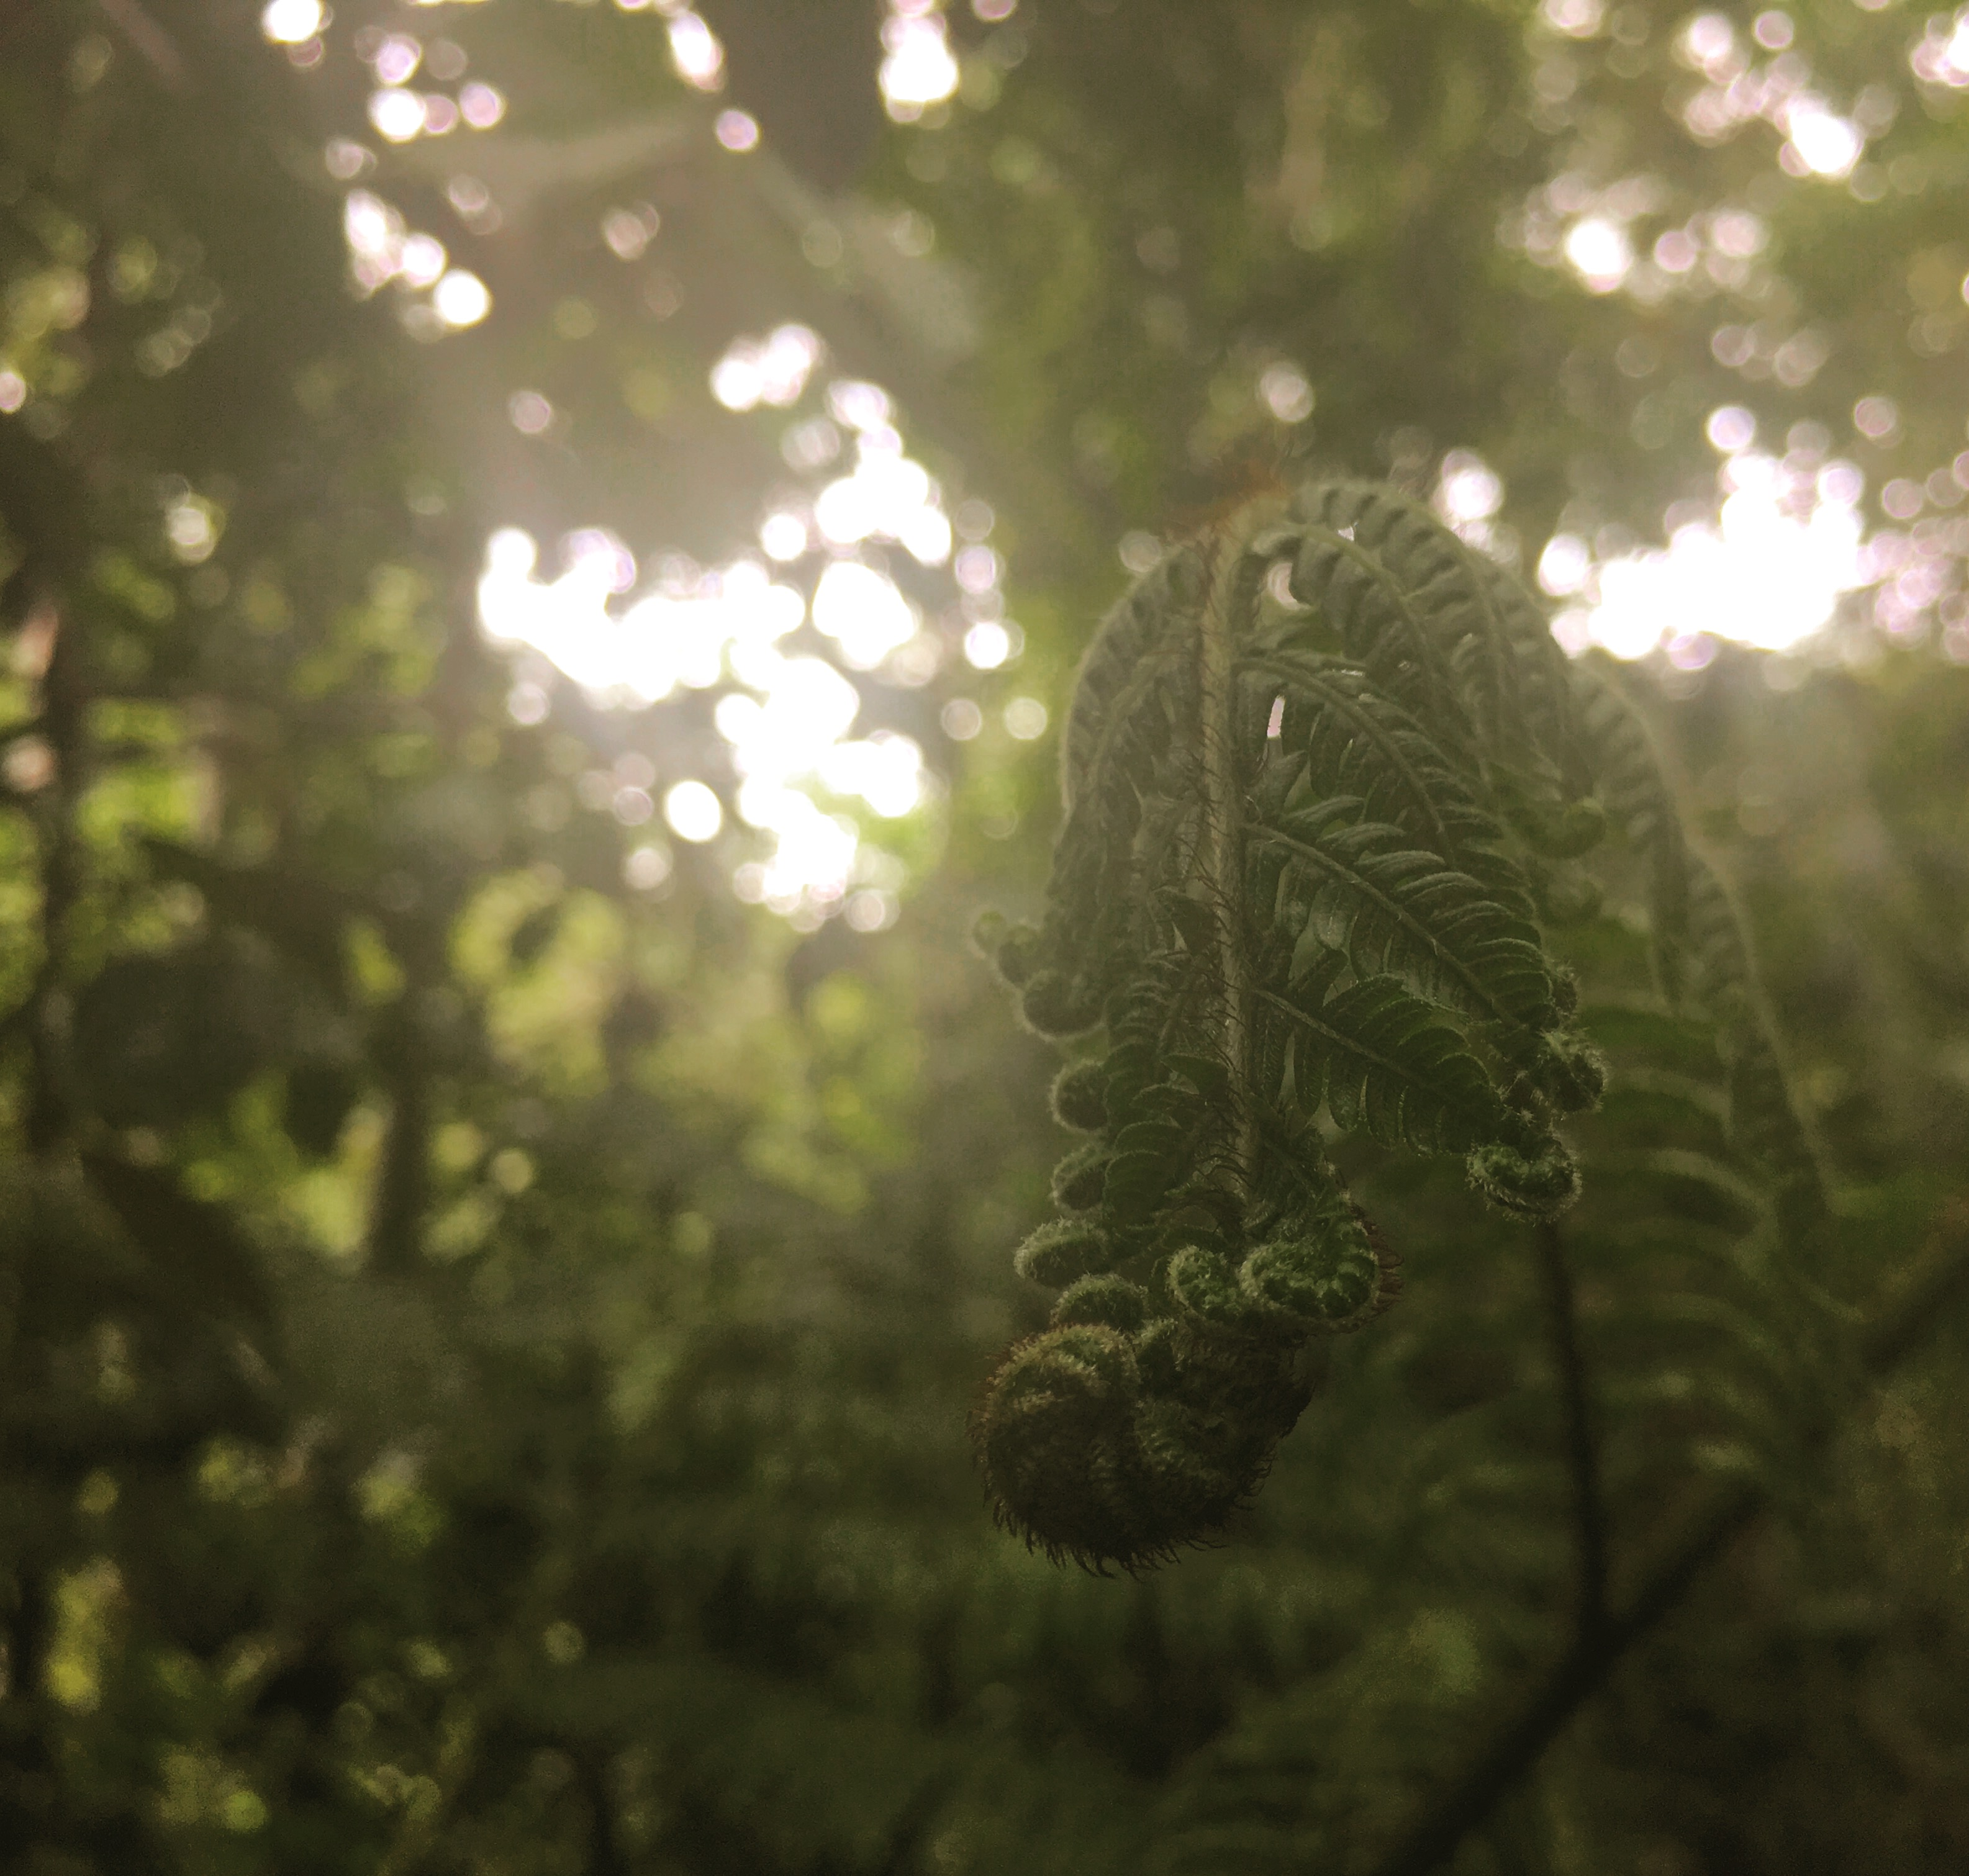
\includegraphics[width=\textwidth,trim={18cm 0 27cm 0},clip]{img/tropical_fern}
\end{center}
\end{column}
\end{columns}
\end{frame}

\begin{frame}{Closing Thoughts: Scientific Questions}
\begin{columns}
\begin{column}{0.6\textwidth}
\begin{itemize}
\item evolutionary biology provides continuing inspiration for new techniques in evolutionary computing
\item evolutionary models move theory evaluation from a qualitative endeavor towards a quantitative endeavor
\end{itemize}
\end{column}
\begin{column}{0.4\textwidth}
\begin{center}
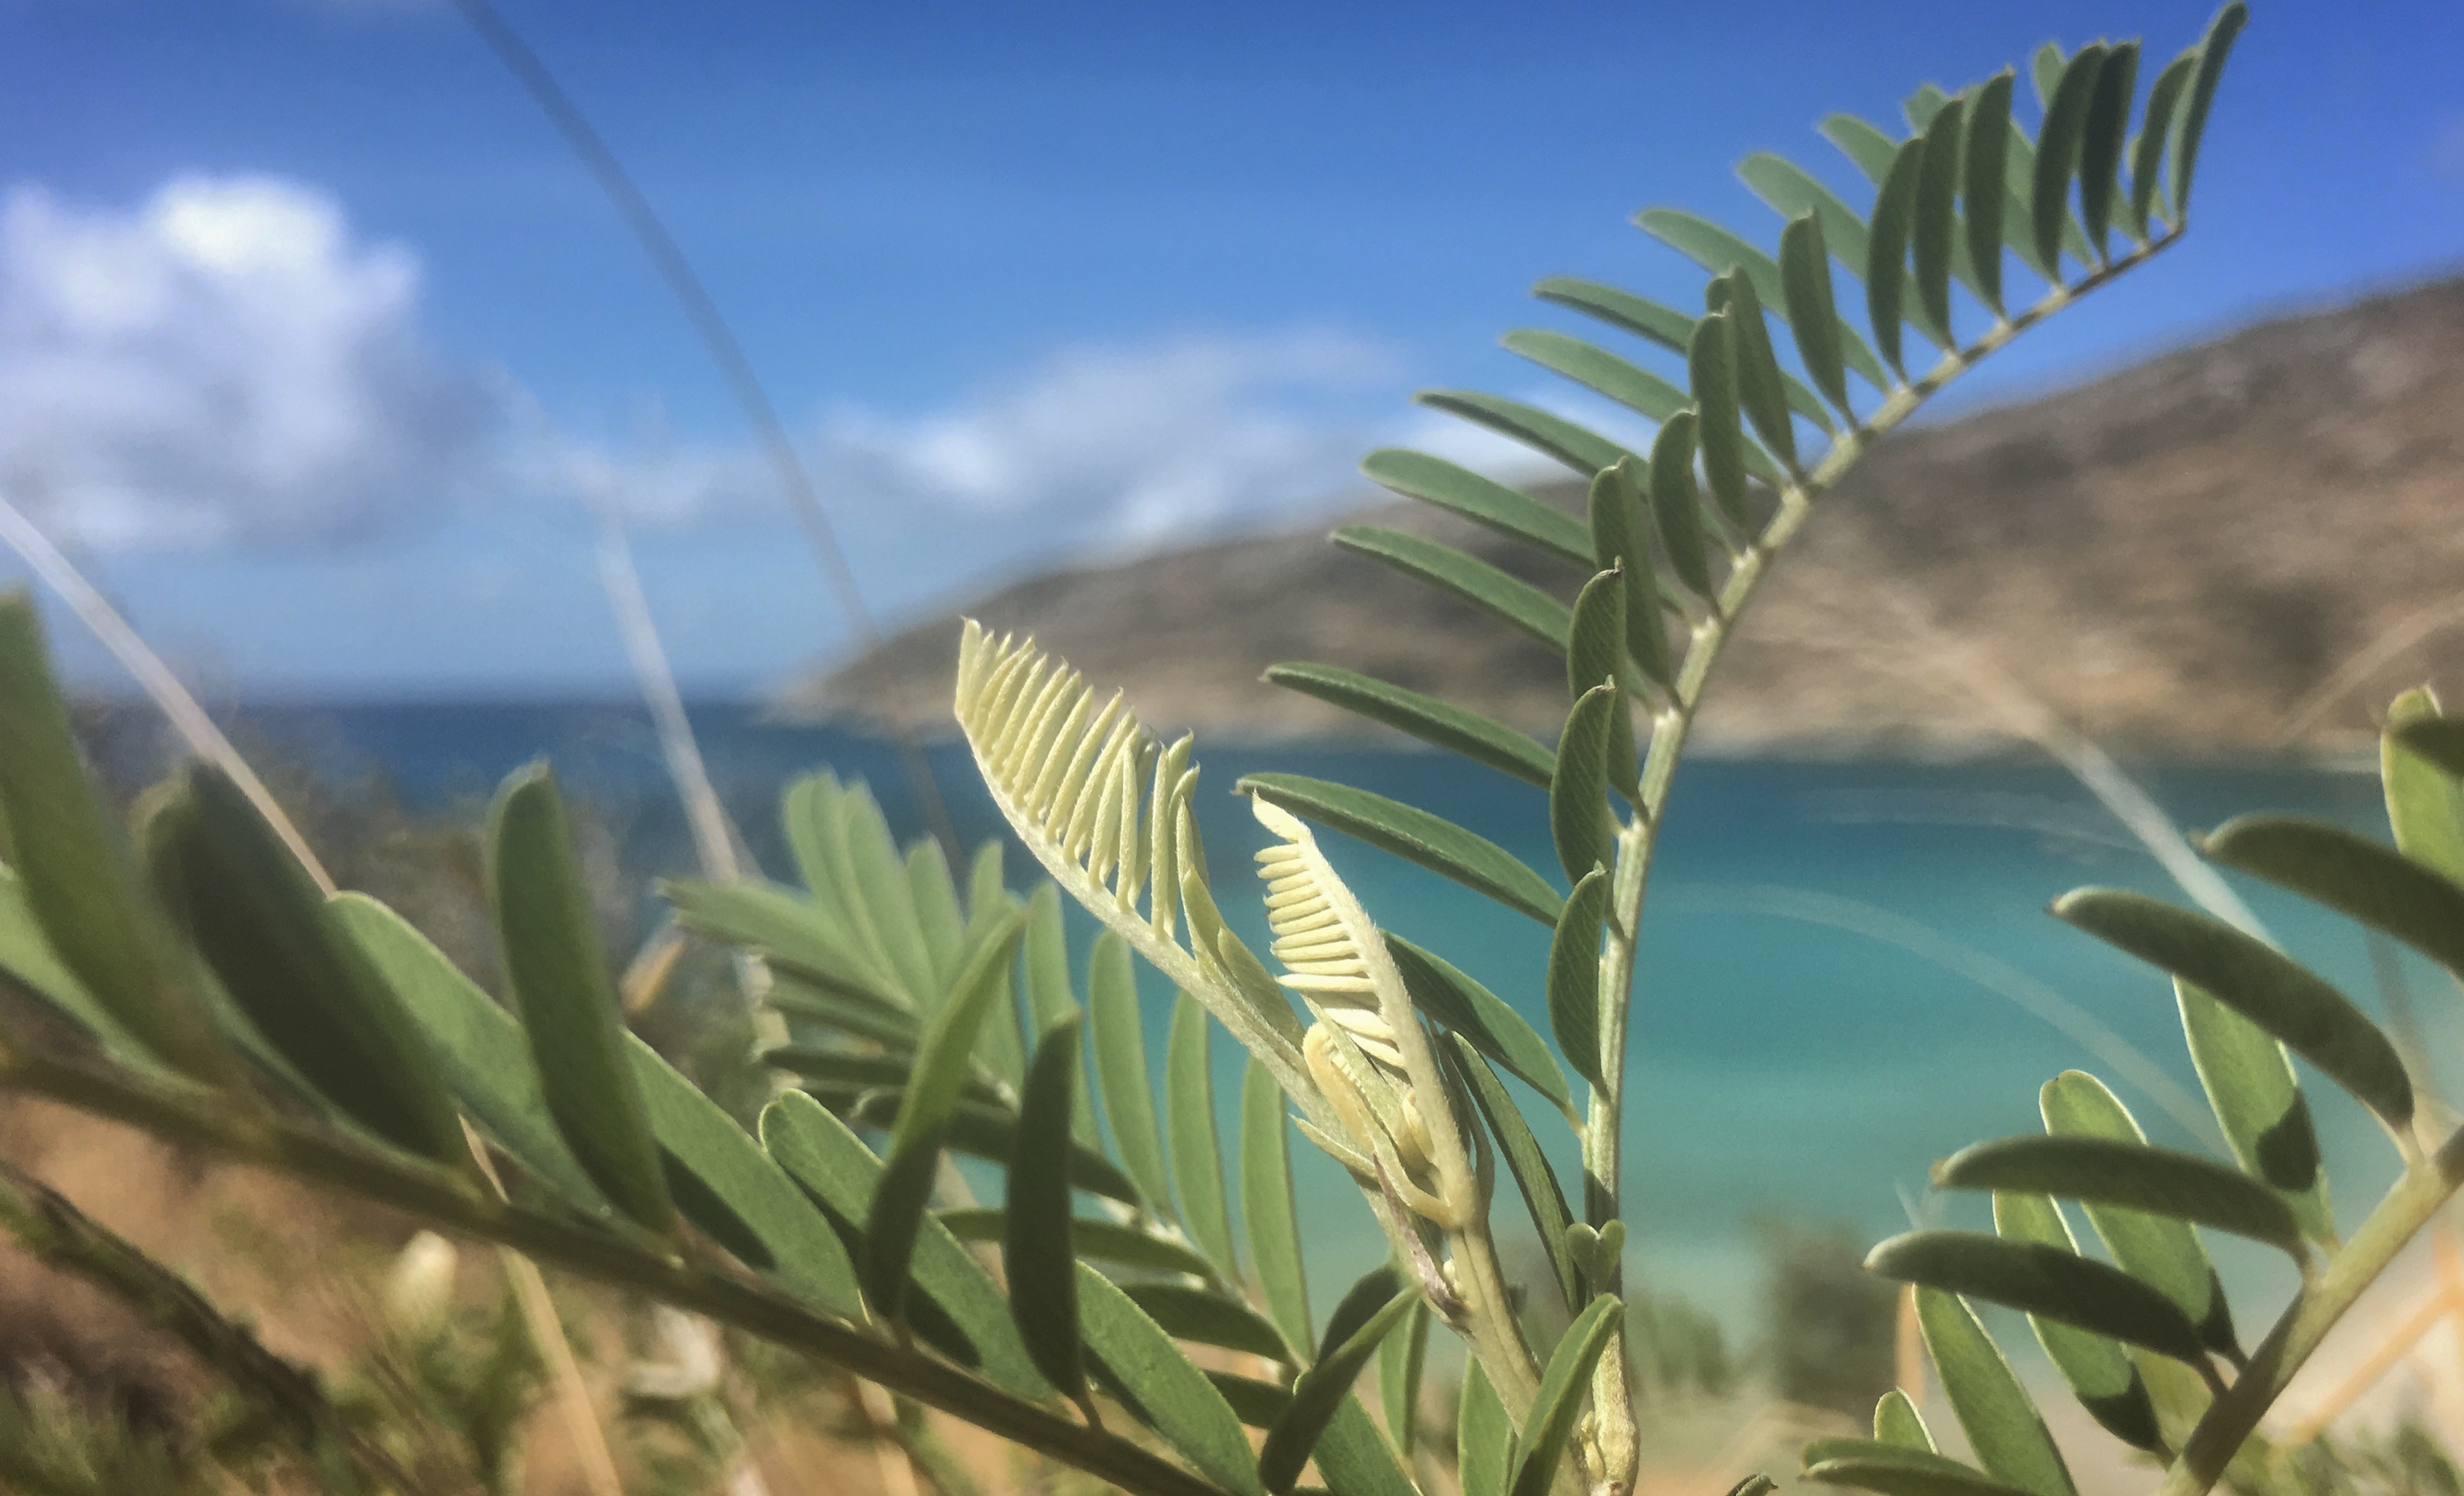
\includegraphics[width=\textwidth,trim={43cm 0 47cm 0},clip]{img/island_fern}
\end{center}
\end{column}
\end{columns}
\end{frame}

% \begin{frame}{Scientific Questions}
% \begin{displayquote}
% ``Many evolutionary biologists do not see a need to connect somatic adaptability to the generation of variation, and some see a need to keep them separate. For them, it is sufficient to say that random mutation is required and that the phenotypic variation arises haphazardly from it as random damage; the organism's current phenotype does not matter for the variation produced, and the output of variation is nearly random \cite[p 219]{Kirschner2005TheDilemma}.''
% \end{displayquote}
% \end{frame}

\section{Causes of Evolvability: Intuition}

\begin{frame}{Summary}
  \alert{big idea}: internal system configuration determines the outcomes of change to the system
\end{frame}


\begin{frame}{Computer Science Intuition: Spaghetti Code}
  idea: software without compartmentalization, error handling, with hard-coded constants, etc. is much more difficult to alter in useful ways
  \begin{figure}
  \centering
  \begin{subfigure}[b]{0.5\textwidth}
    \centering
    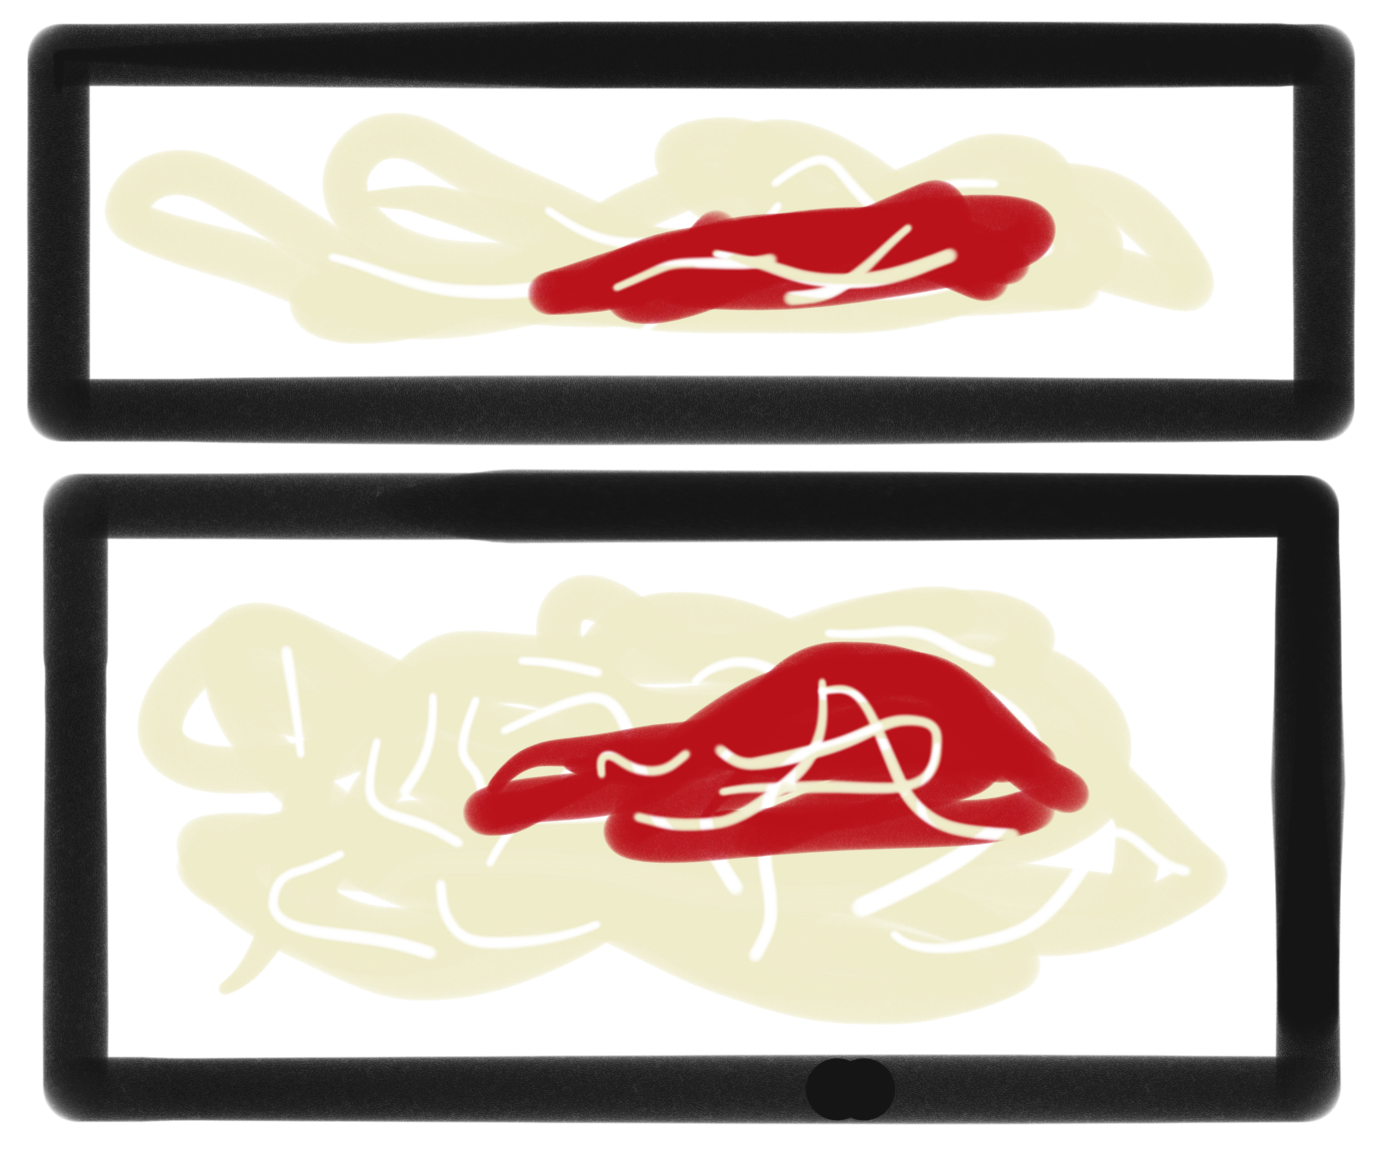
\includegraphics[width=\textwidth]{img/spaghetticode}
    \caption{spaghetti code}
    \label{subfig:spaghetti_code}
  \end{subfigure}%
  \hfill
  \begin{subfigure}[b]{0.5\textwidth}
    \centering
    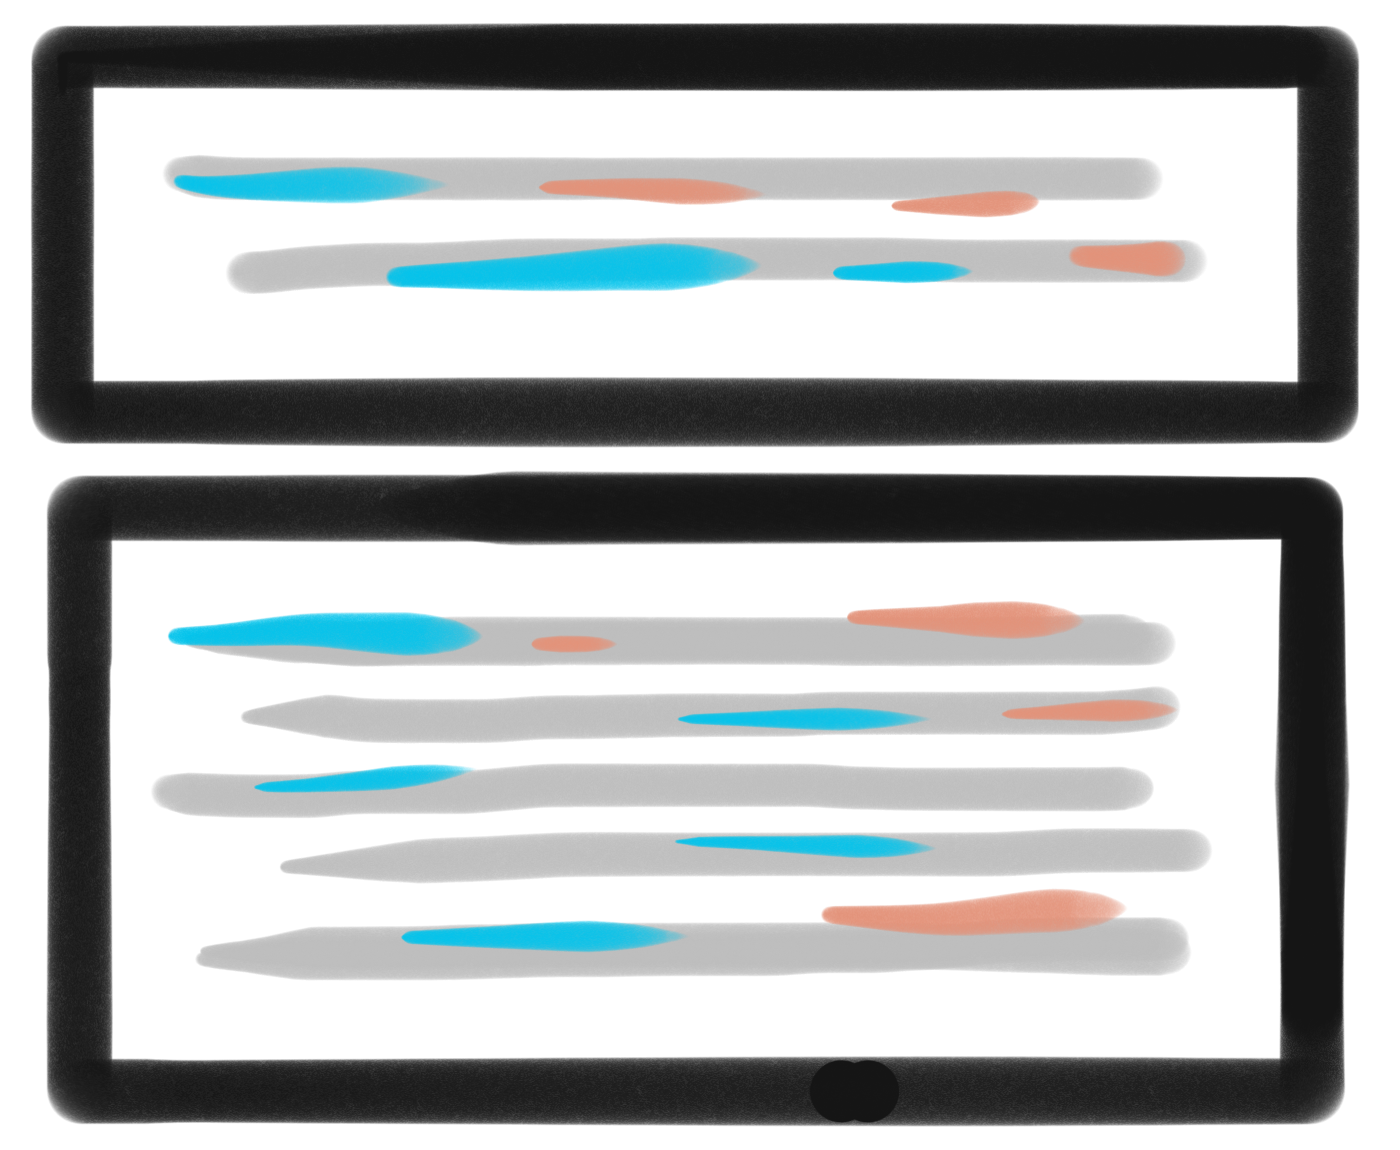
\includegraphics[width=\textwidth]{img/regularcode}
    \caption{regular code}
     \label{subfig:regular_code}
  \end{subfigure}
  \captionsetup{singlelinecheck=off,justification=raggedright}
  \caption{A cartoon comparison of spaghetti and regular code.}
  \label{fig:direct_irregular_vs_indirect_regular}
\end{figure}
\end{frame}

\begin{frame}{Analysis}
\begin{itemize}
	\item environmental noise $\rightarrow$ noise mitigation structures $\rightarrow$ more silent mutations
    \item alternate phenotypic targets $\rightarrow$ developmental path switching structures $\rightarrow$ fewer silent mutations
    \item how will noise mitigation structure and developmental path switching structures interact?
 \end{itemize}
\end{frame}


\section{Project Schedule}


\begin{frame}{Last Few Weeks (old plan)}
\begin{center}
{\centering ~$\bm{\vdots}$~}
\end{center}
\begin{itemize}
  \item \textbf{Week 11} perform experiments with indirect plasticity
  \item \textbf{Week 12} perform combined experiments with indirect and direct plasticity
  \item \textbf{Week 13} network structure analysis
  \begin{itemize}
    \item \textit{Monday April 10th}: Math/CS Department presentation
  \end{itemize}
  \item \textbf{Week 14} prepare for Math/CS Day presentation, capstone writeup
  \item \textbf{Week 15} prepare for Math/CS Day presentation, capstone writeup
  \begin{itemize}
  	\item \textit{Saturday April 29th}: Math/CS Day presentation
  \end{itemize}
 \end{itemize}
\vspace{-1ex}
\begin{center}
{\centering ~$\bm{\vdots}$~}
\end{center}
\end{frame}

\begin{frame}{Last Few Weeks (new plan)}
\begin{center}
{\centering ~$\bm{\vdots}$~}
\end{center}
\begin{itemize}
  \item \textbf{Week 11} perform experiments with indirect plasticity
  \item \textbf{Week 12} prepare for Math/CS Day presentation
  \item \textbf{Week 13} prepare for Math/CS Day presentation
  \begin{itemize}
    \item \textit{Monday April 10th}: Math/CS Department presentation
  \end{itemize}
  \item \textbf{Week 14} perform combined experiments with indirect and direct plasticity
  \item \textbf{Week 15} network structure analysis
  \begin{itemize}
  	\item \textit{Saturday April 29th}: Math/CS Day presentation
  \end{itemize}
 \end{itemize}
\vspace{-1ex}
\begin{center}
{\centering ~$\bm{\vdots}$~}
\end{center}
\end{frame}

\appendix

\begin{frame}[standout]
  Questions?
\end{frame}

\begin{frame}[allowframebreaks]{References}

  \bibliography{Mendeley}
  \setbeamertemplate{bibliography item}{\insertbiblabel}
  %\nocite{*} % Insert publications even if they are not cited in the poster
  \bibliographystyle{apalike}
\end{frame}


\begin{frame}{Experimental Questions}
\begin{itemize}
\item how do genetic regulatory networks evolved with direct plasticity differ structurally from control networks? \cite{Reisinger2007AcquiringRepresentations}
\item impact of other modes of direct plasticity on evolvability (rule noise, fixed states, intermediate state perturbation)?
\item impact of indirect plasticity on evolvability?   
\item combined impact of direct and indirect plasticity on evolvability?   
\end{itemize}
\end{frame}


\begin{frame}{Generating and Reading an Evolvability Signature}
  \begin{figure}
  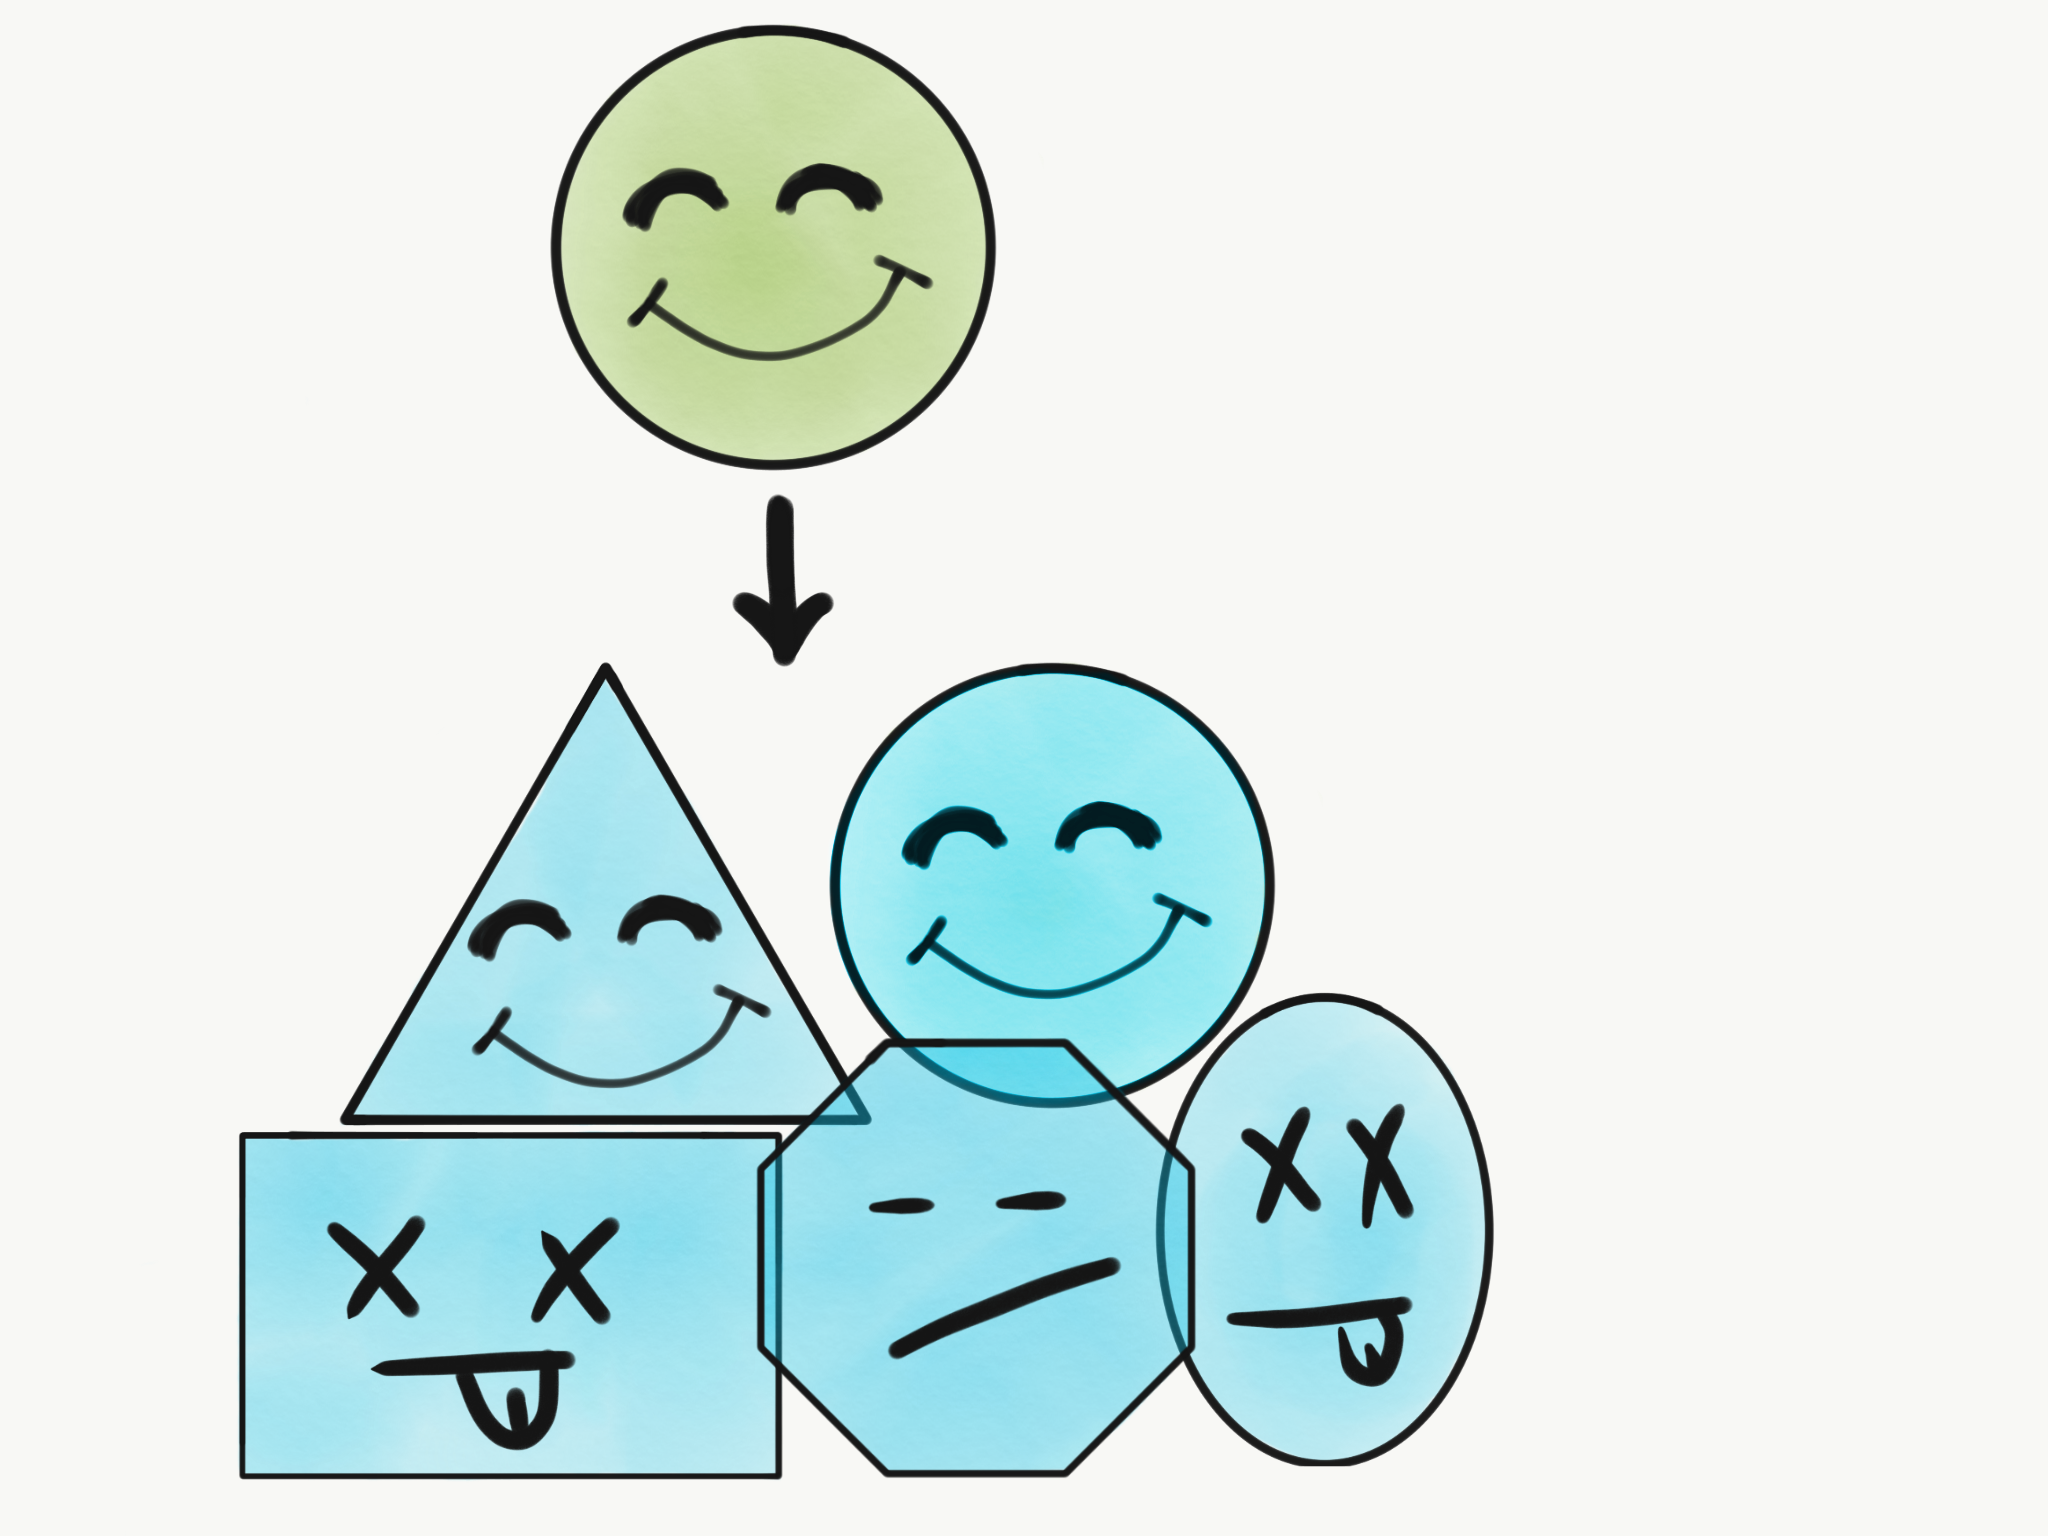
\includegraphics[width=0.5\textwidth]{img/evol_sig_gen}
  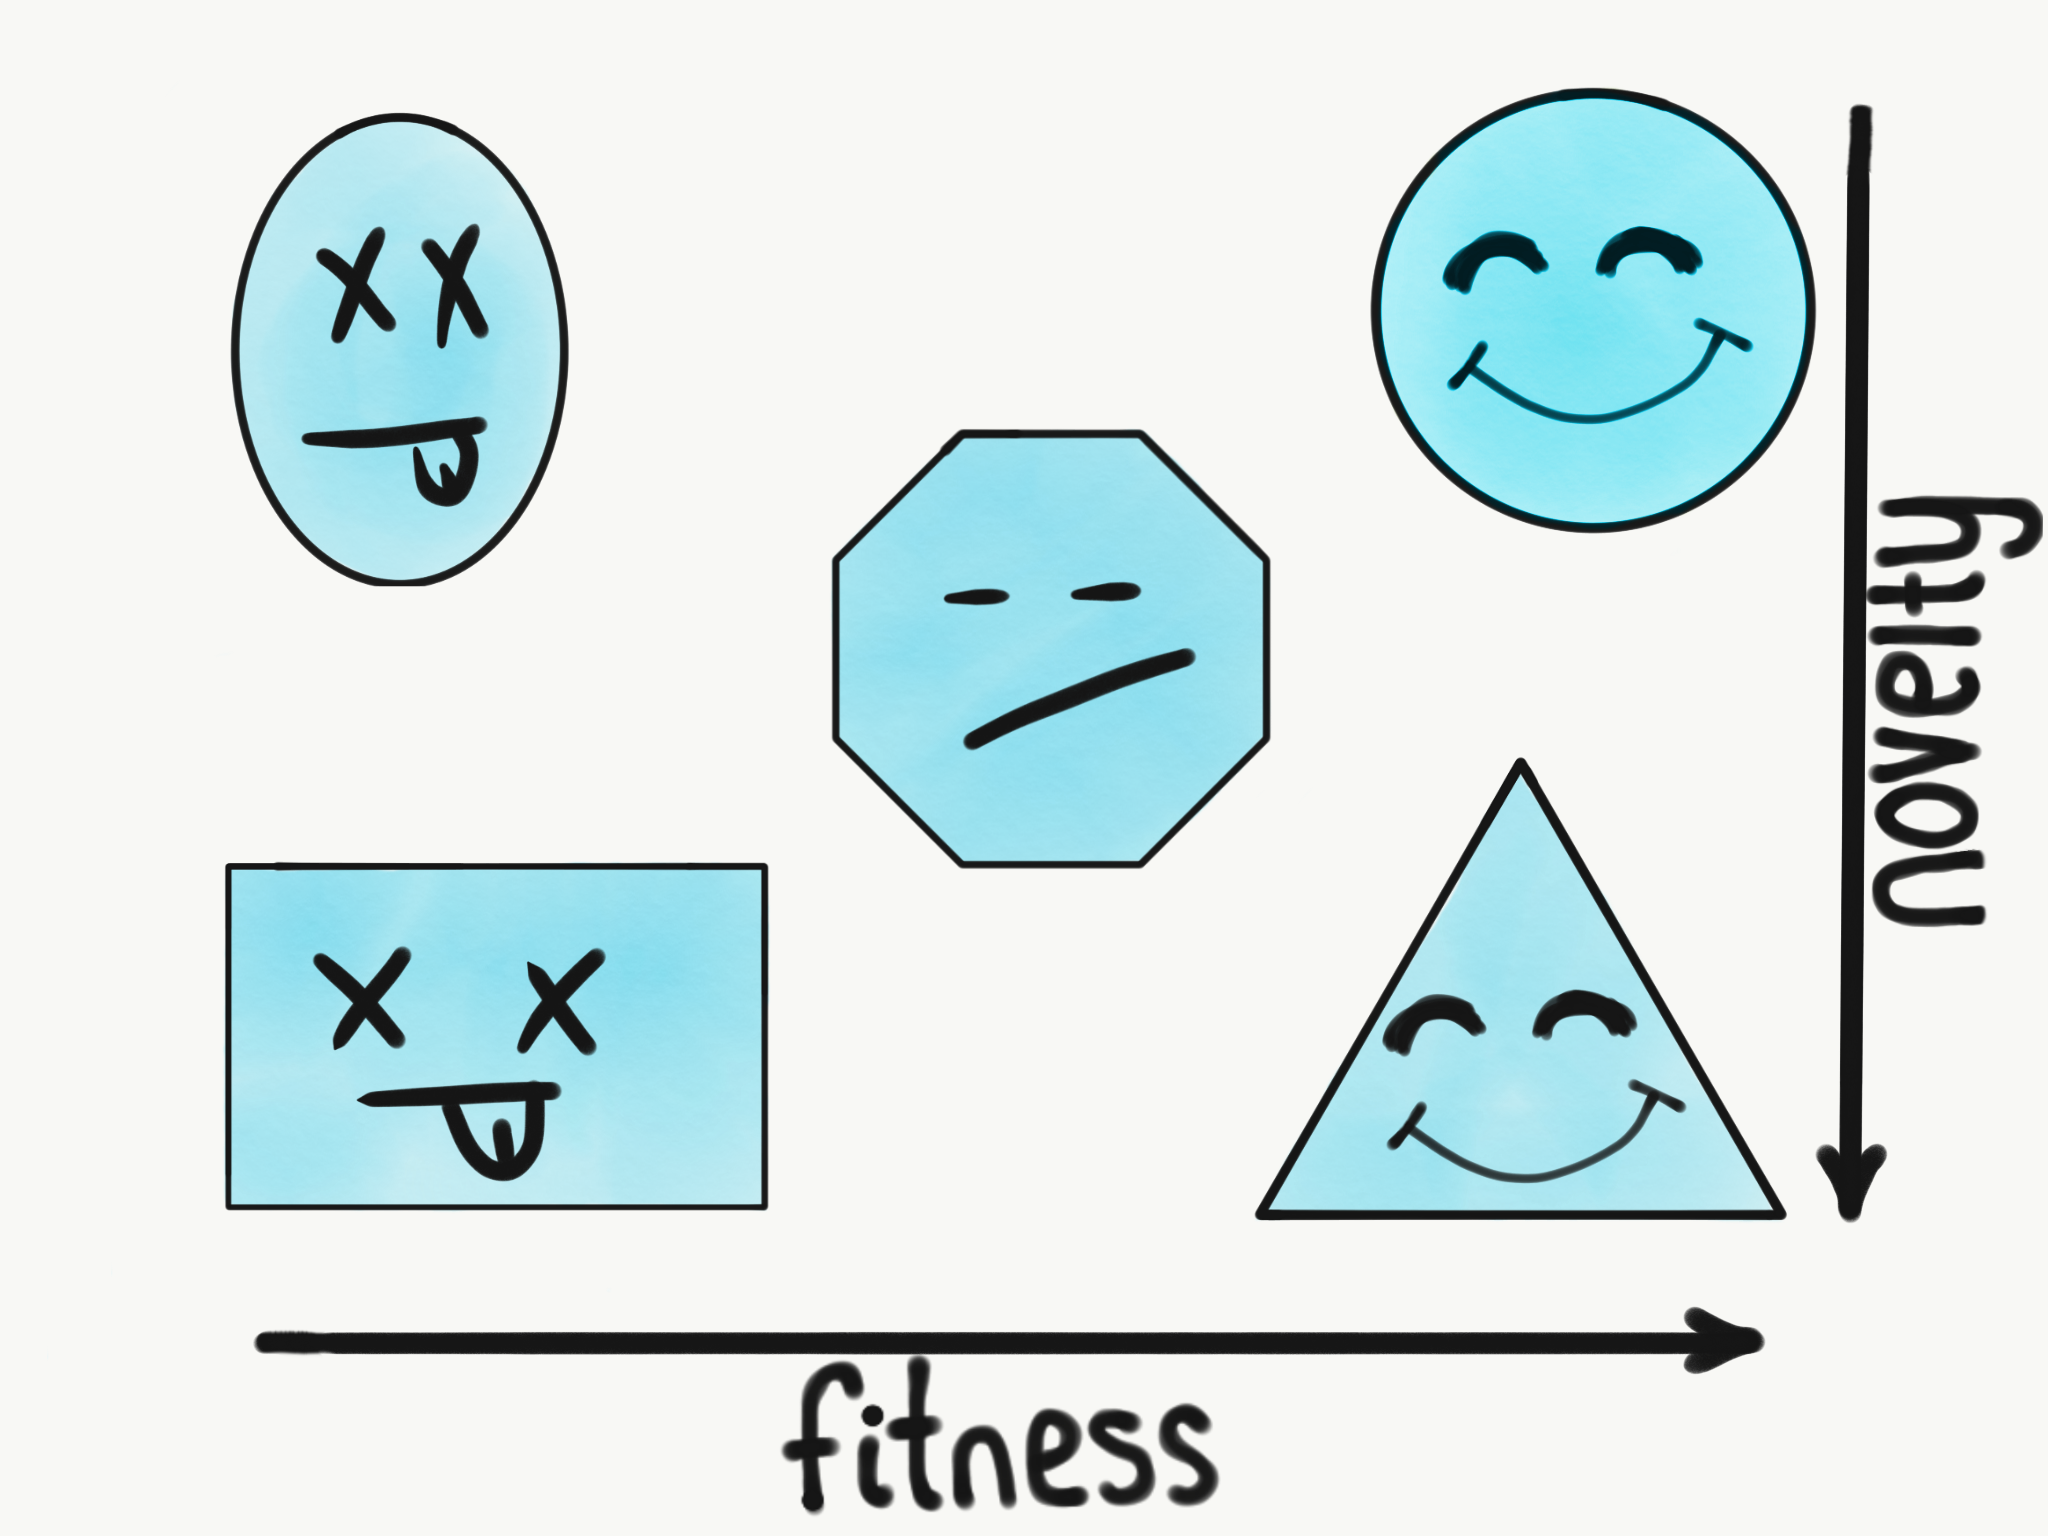
\includegraphics[width=0.5\textwidth]{img/evol_sig_read}
  \captionsetup{singlelinecheck=off,justification=raggedright}
  \caption{Cartoon illustration describing the creation and layout of an evolvability signature diagram \cite{Tarapore2015EvolvabilityBenchmarks}.}
  \label{fig:reading_evolvability_signature}
\end{figure}
\end{frame}

\begin{frame}{Evolvability Visualization $W=0$} 
\begin{figure}
    \centering
    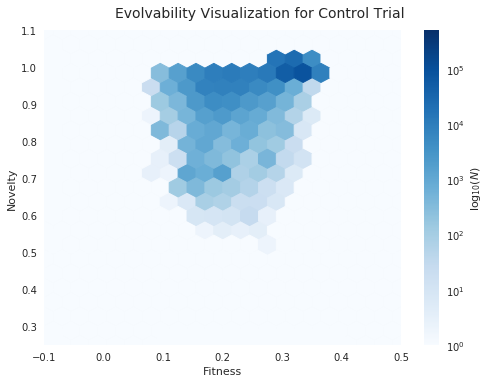
\includegraphics[width=0.8\textwidth]{img/ev_w0}
 	\captionsetup{singlelinecheck=off,justification=raggedright}
  	\caption{Evolvability visualization of champions evolved with only a primary condition/objective pair.}
    \label{fig:ev_w0}
\end{figure}
\end{frame}

\begin{frame}{Evolvability Visualization $W=0.2$}
\begin{figure}
    \centering
    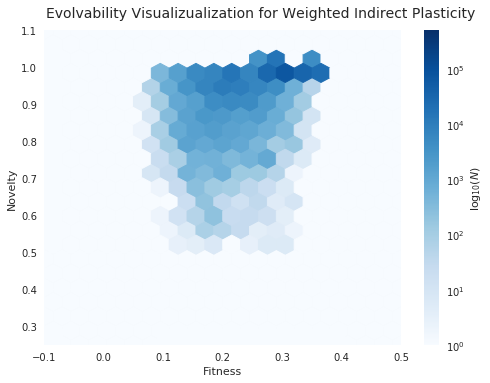
\includegraphics[width=0.8\textwidth]{img/ev_w0_2}
 	\captionsetup{singlelinecheck=off,justification=raggedright}
  	\caption{Evolvability visualization of champions evolved with primary and secondary condition/objective pairs.}
    \label{fig:es_w0_2}
\end{figure}
\end{frame}


\begin{frame}{Environmental Influence on the Phenotype}
\begin{itemize}
	\item in biology, genotype not sole determinant of phenotype
    \item $P = G + E$
    \item plasticity: phenotypic response to the environment
    \item direct plasticity versus indirect plasticity
\end{itemize}
\end{frame}

\begin{frame}{Direct Plasticity: Biological Intuition}
  \begin{figure} \label{fig:elephant_developmental_perturbation}
  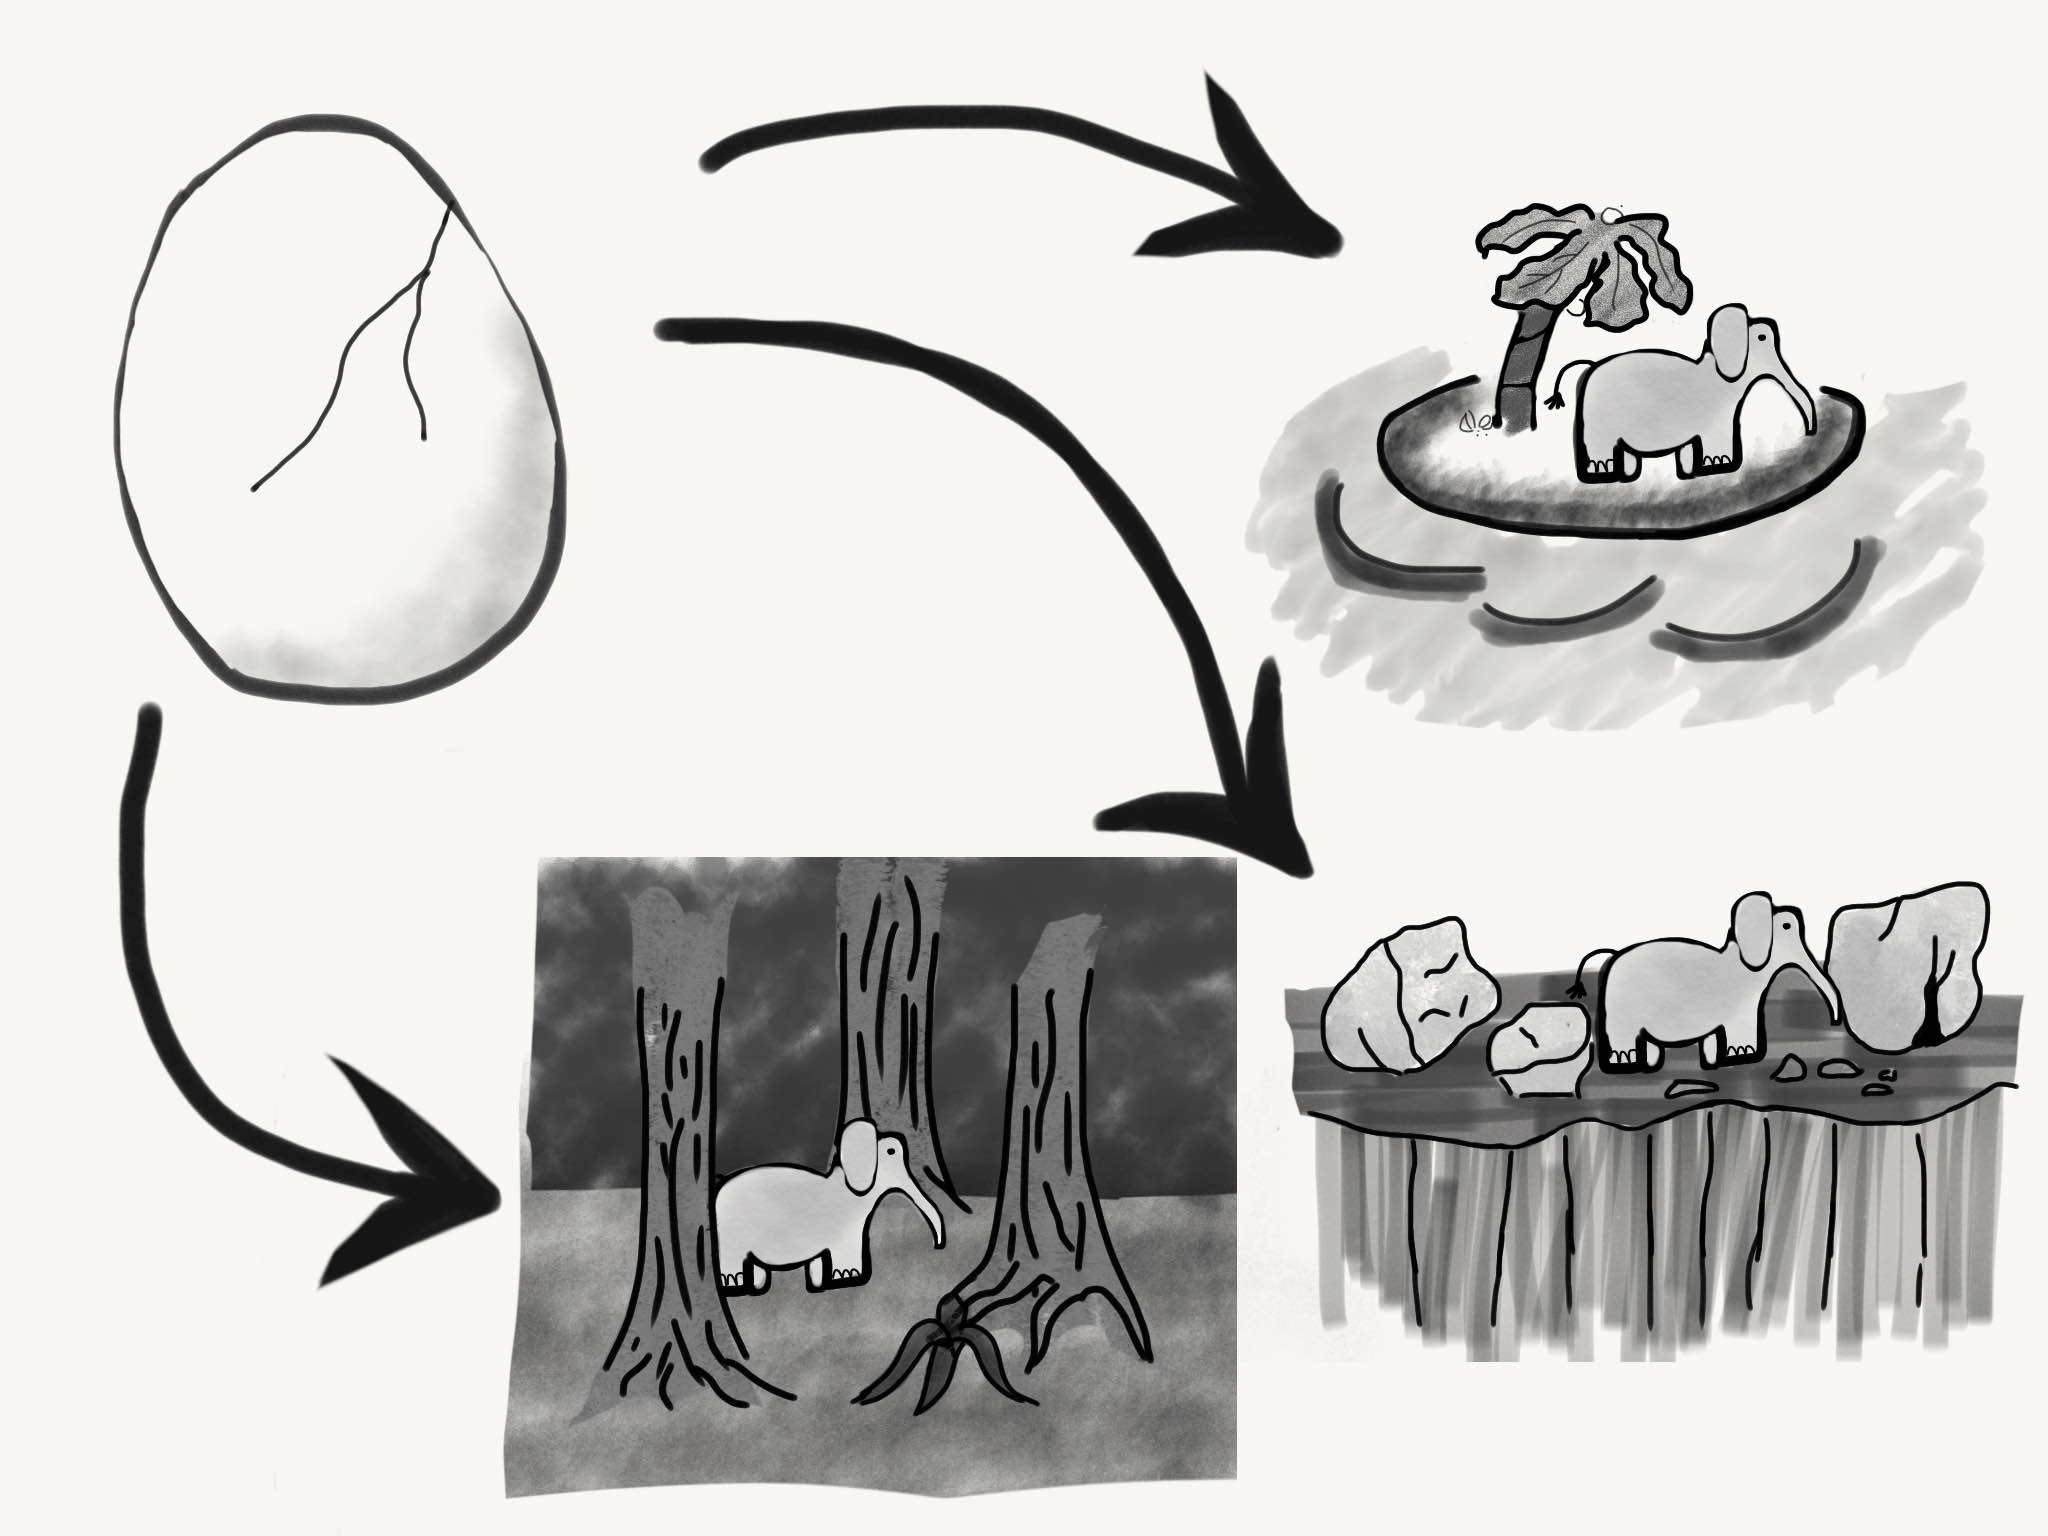
\includegraphics[width=0.8\textwidth]{img/elephant_developmental_perturbation.jpg}
  \captionsetup{singlelinecheck=off,justification=raggedright}

  \caption{A cartoon illustration of resistance to environmental perturbation.}
\end{figure}
\end{frame}

\begin{frame}{Indirect Plasticity: Biological Intuition}
  \begin{figure} \label{figs/plant_developmental_perturbation}
  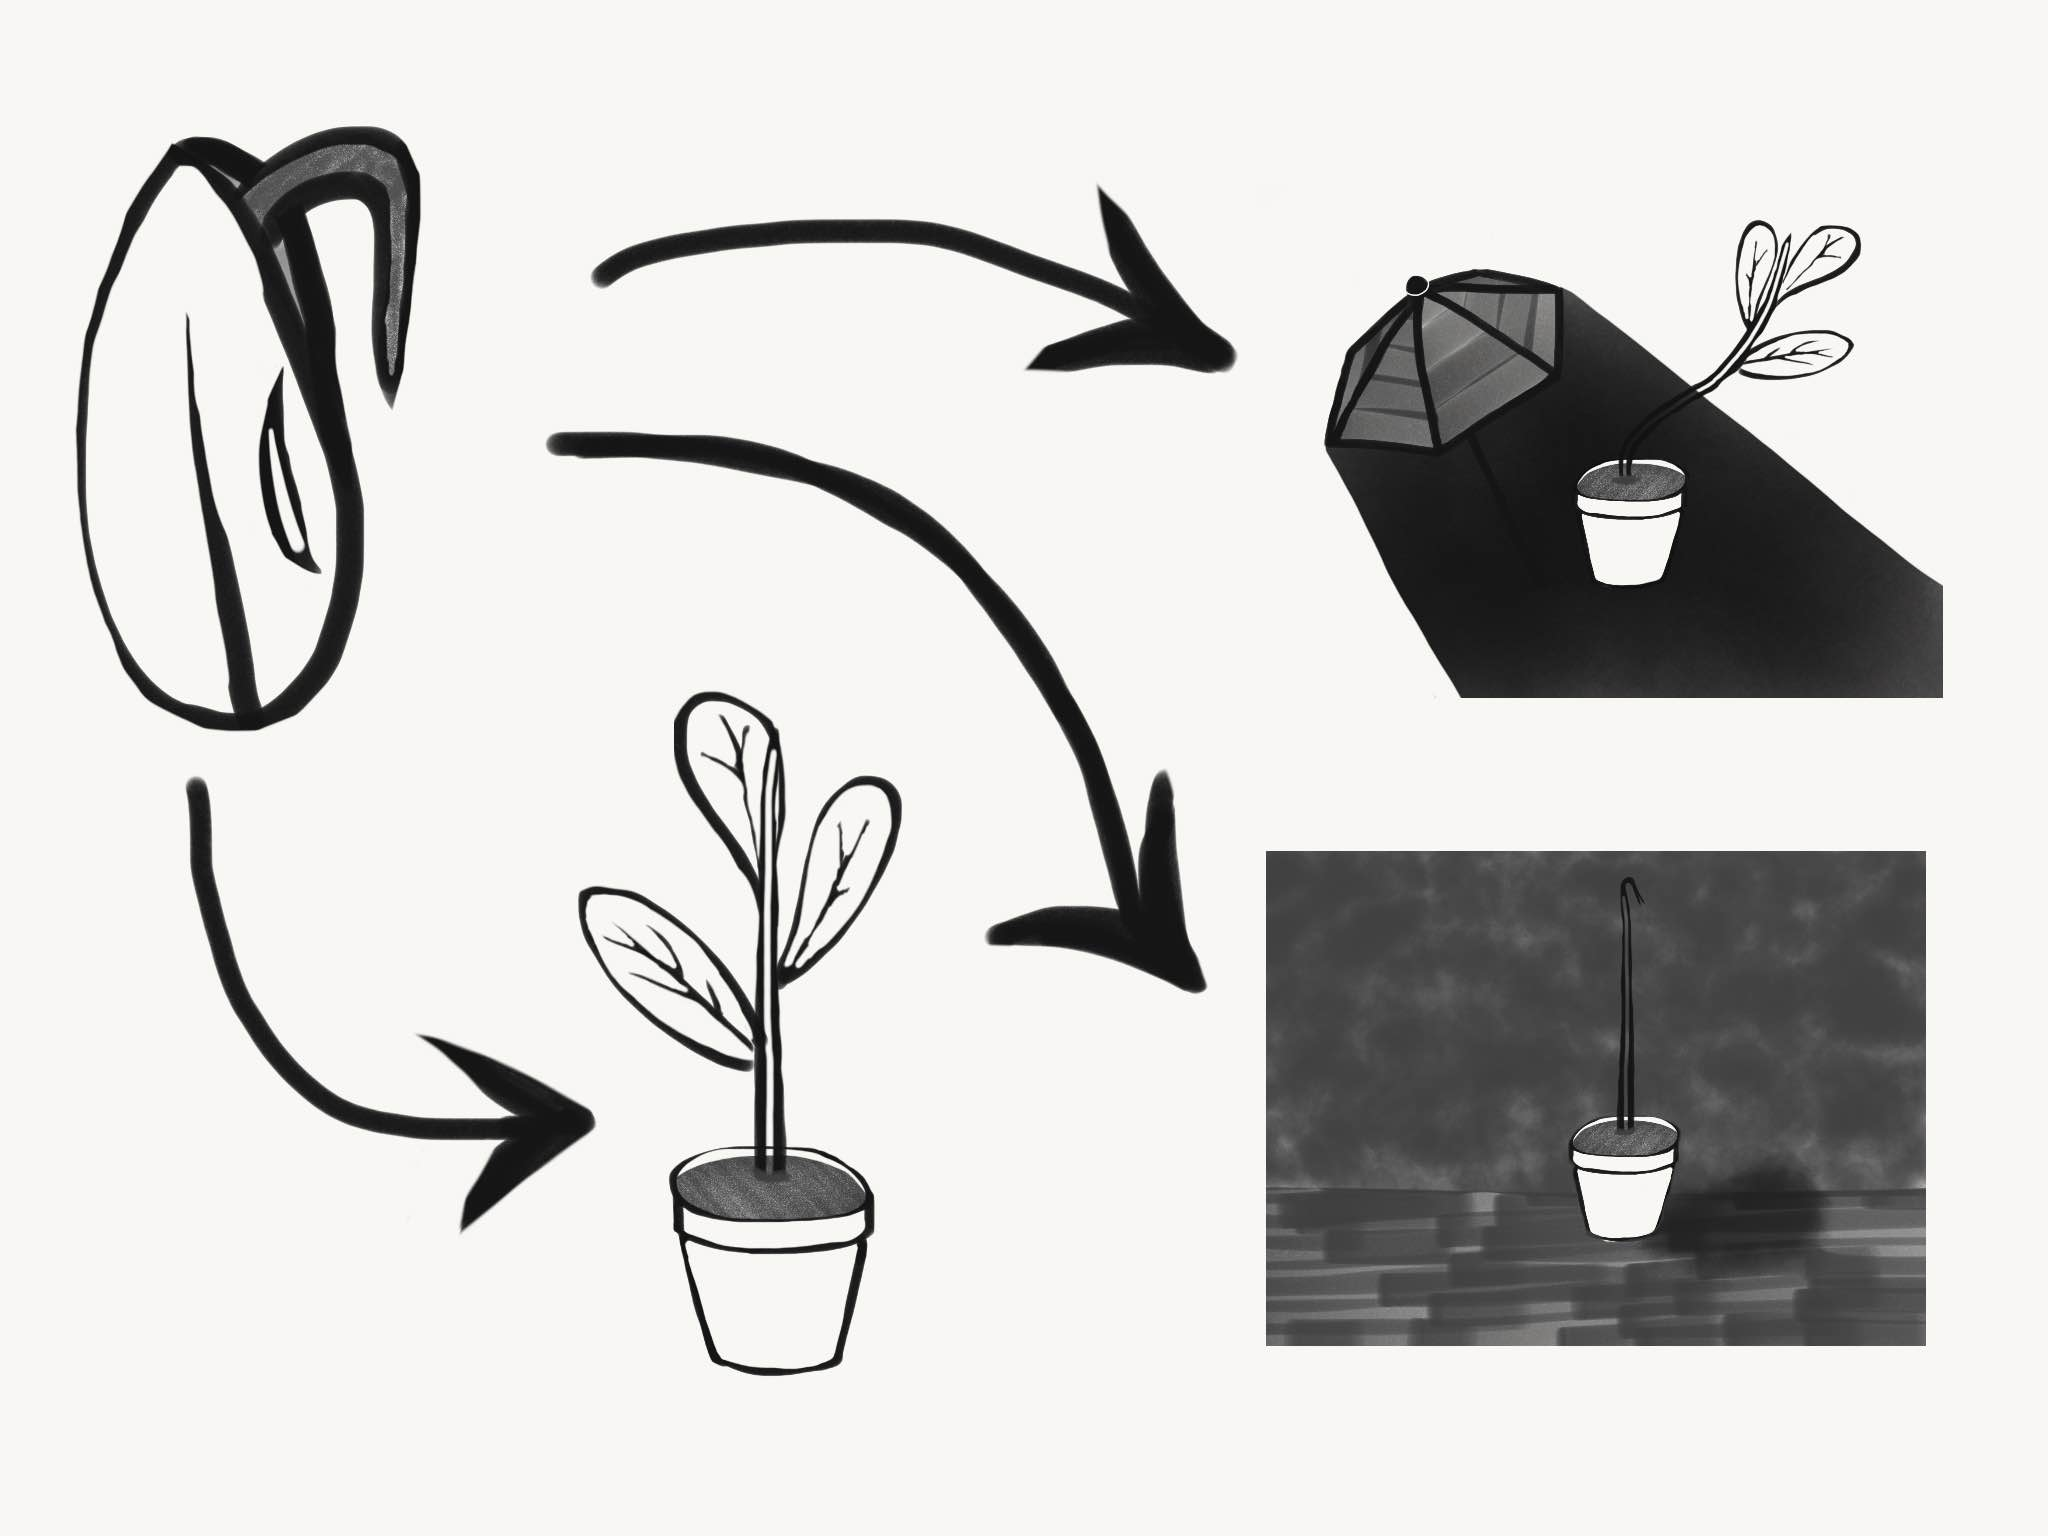
\includegraphics[width=0.8\textwidth]{img/plant_developmental_perturbation.jpg}
  \captionsetup{singlelinecheck=off,justification=raggedright}
  \caption{A cartoon illustration of alternate phenotypes expressed based on environmental signals.}
\end{figure}

\end{frame}

\begin{frame}{Complete Model}
\begin{figure}
    \centering
    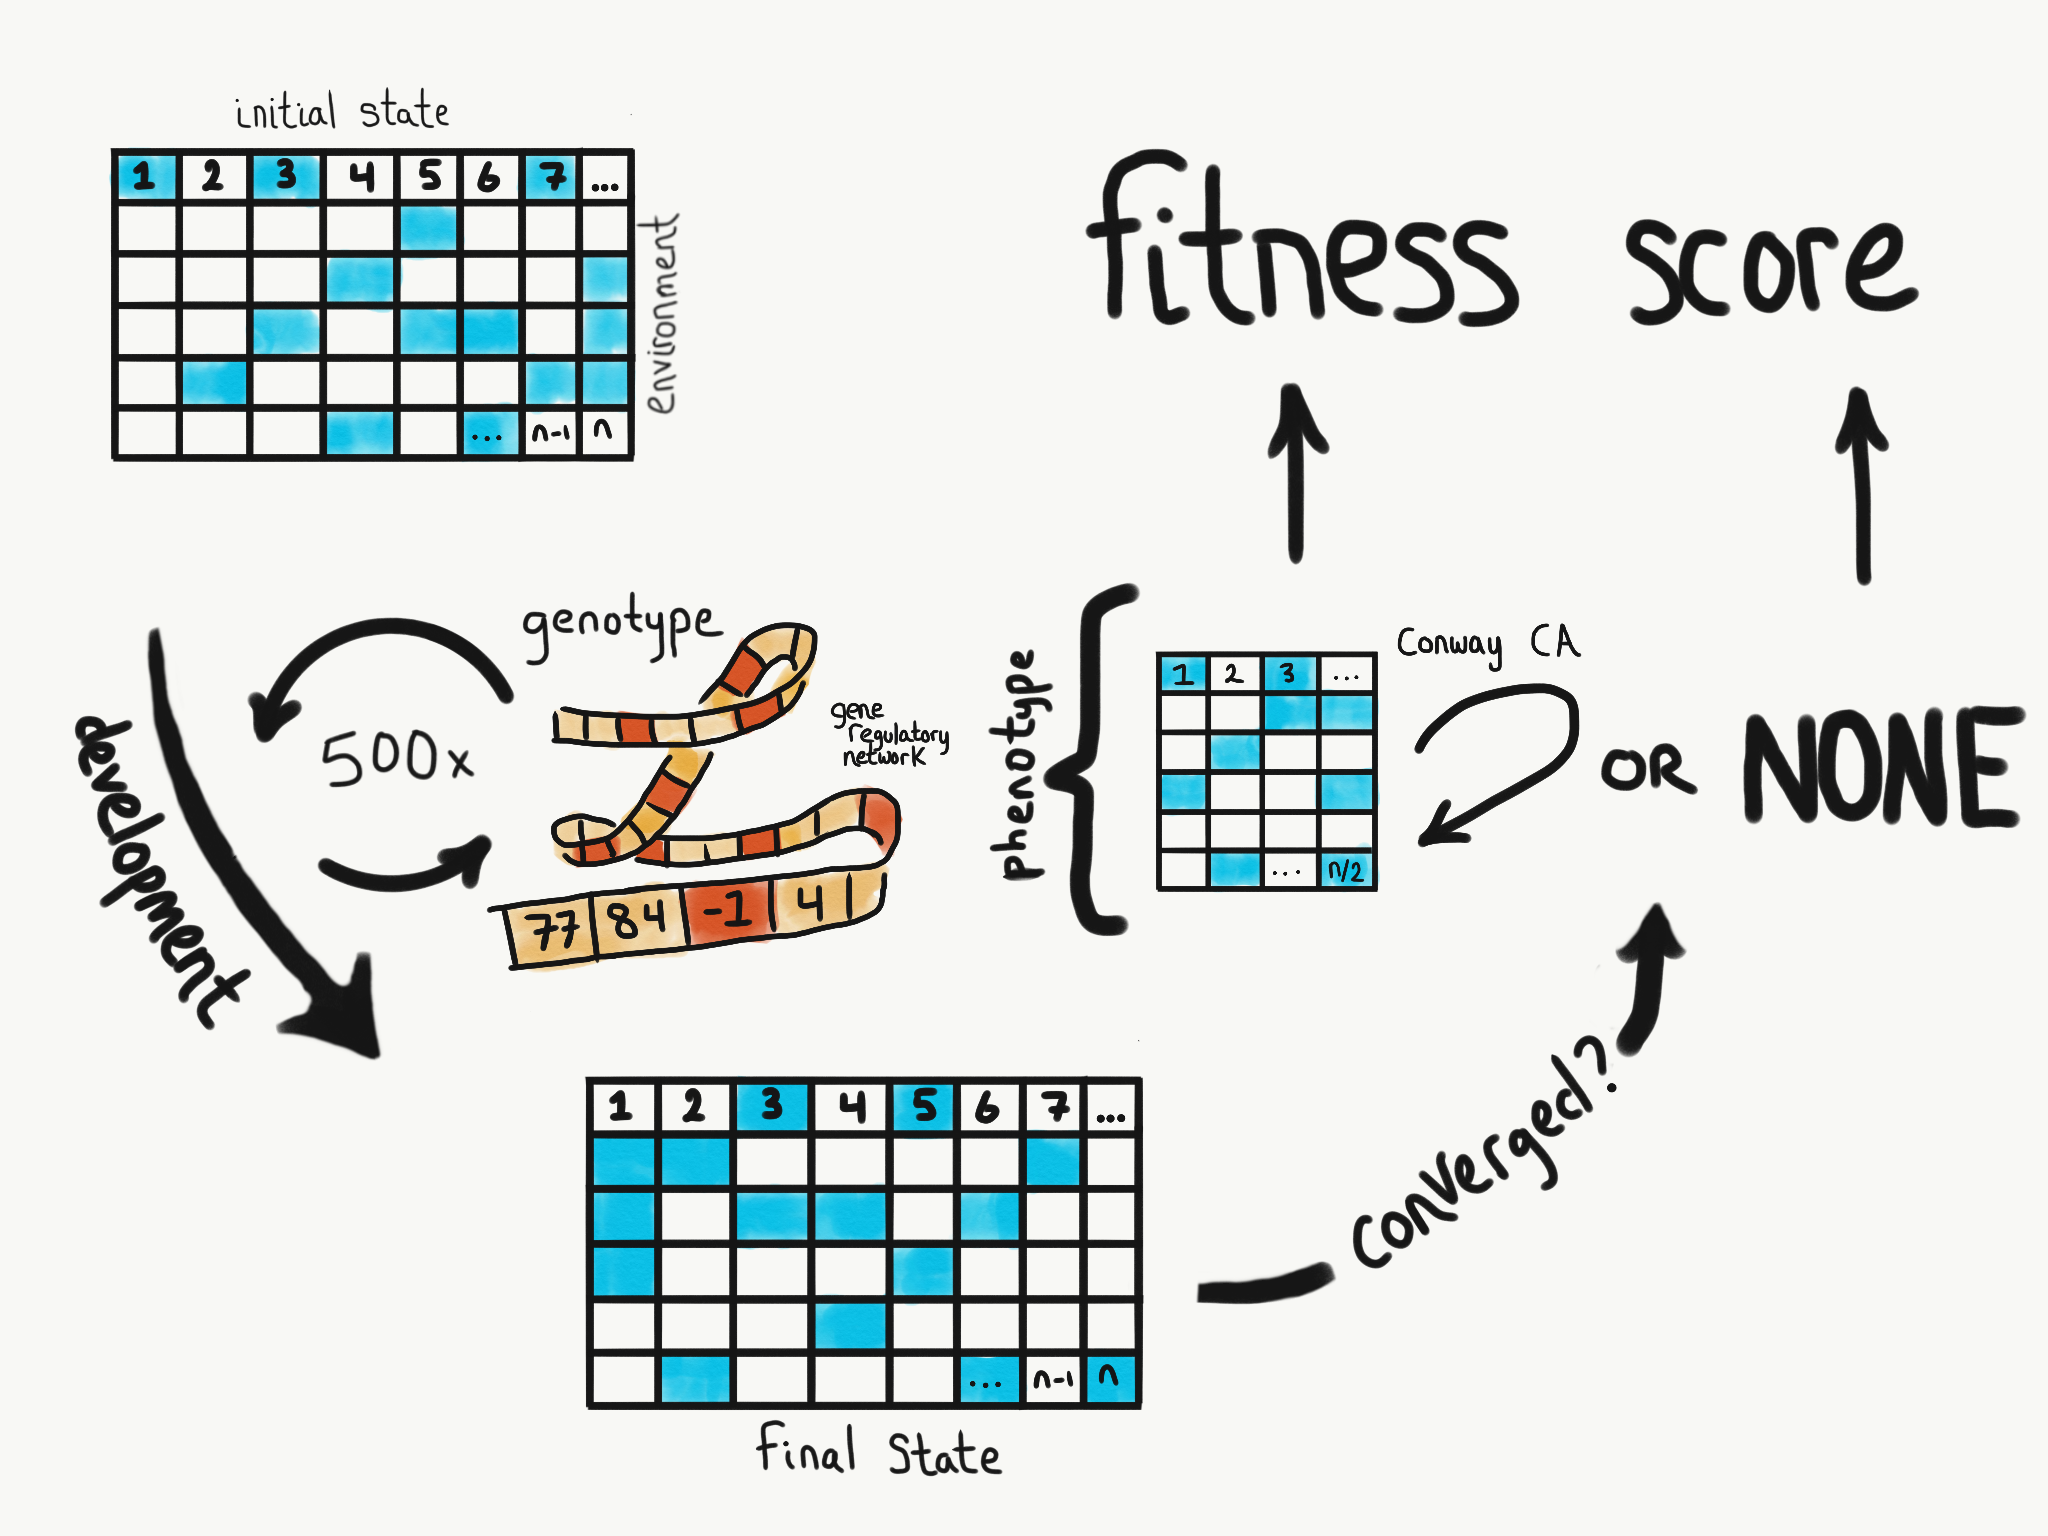
\includegraphics[width=0.8\textwidth]{img/complete_schematic}
 	\captionsetup{singlelinecheck=off,justification=raggedright}
  	\caption{A cartoon overview of the development and assessment processes of the expanded model, based loosely on \cite{Wilder2015ReconcilingEvolvability}.}
    \label{fig:complete_schematic}
\end{figure}
\end{frame}

\begin{frame}{Biological Perspective: Intraindividual Degeneracy}
  idea: employing a diverse collection of substructures that provide identical or near-identical functionality promote robustness through redundancy while providing many jumping off points for variation through repurposing or elaboration
  \begin{figure}
 \begin{columns}
 \begin{column}{0.6\textwidth}
 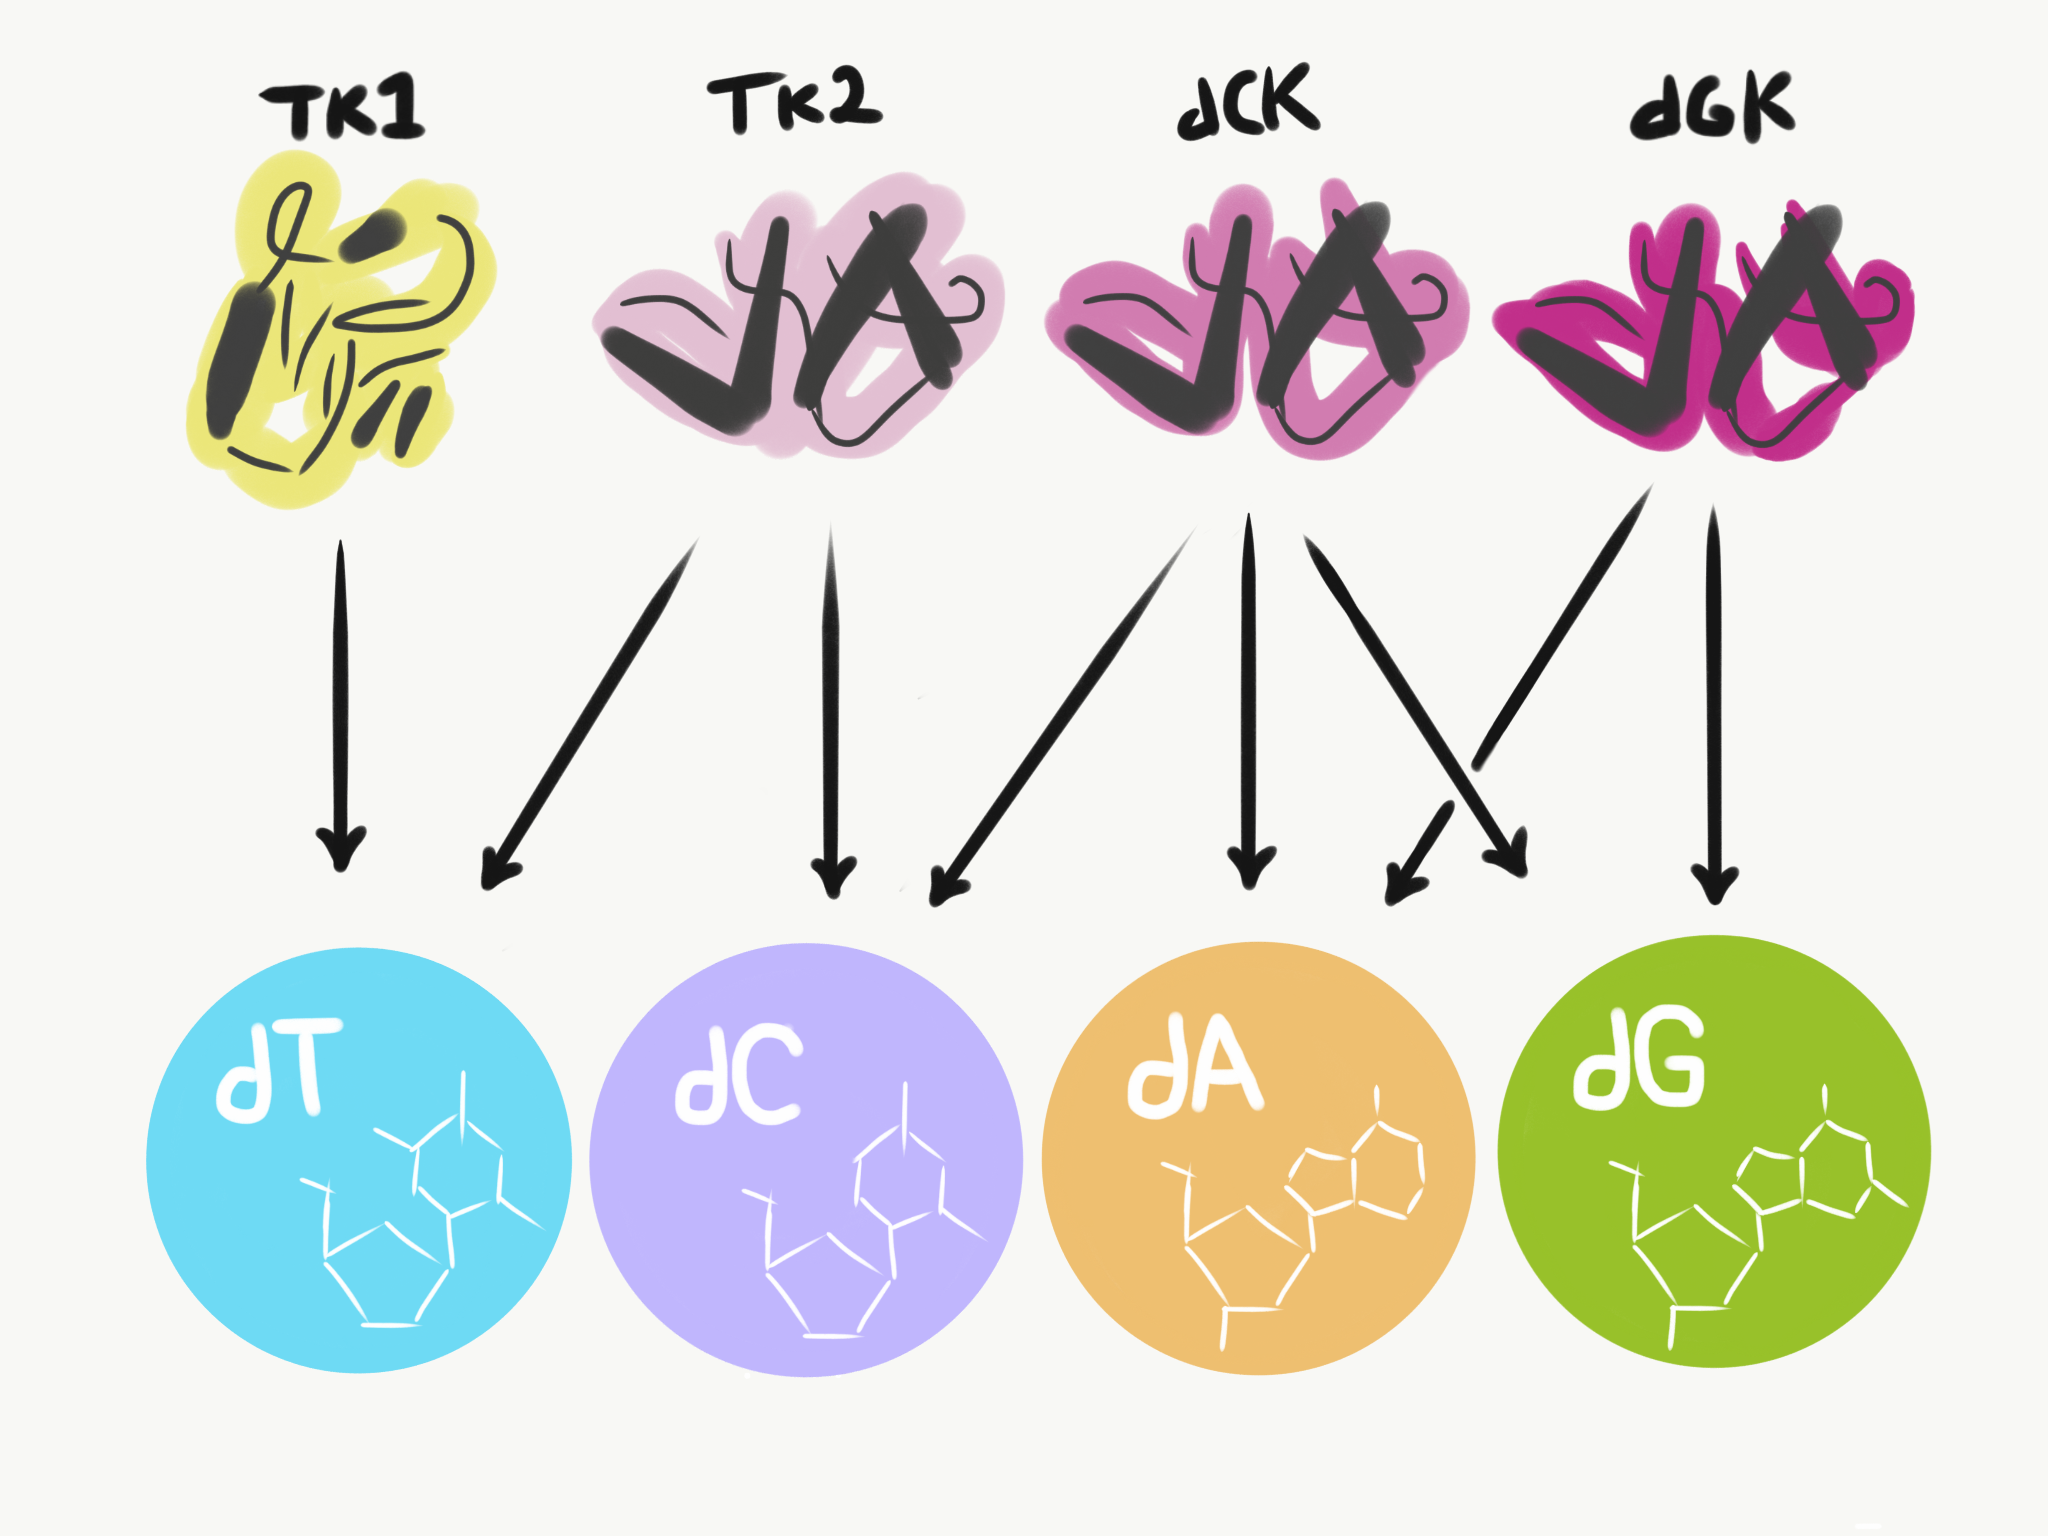
\includegraphics[width=\textwidth]{img/intraindividual_degeneracy}
 \end{column}
 \begin{column}{0.4\textwidth}
\captionsetup{singlelinecheck=off,justification=raggedright}
  	\caption{Mammalian deoxyribonucleoside kinases exhibit degeneracy \cite{Sandrini2005DeoxyribonucleosideReaction.}.}
    \label{fig:intraindividual_degeneracy}
    
\end{column}
\end{columns}
\end{figure}
\end{frame}

\begin{frame}{Conway's Game of Life}
\begin{figure}
  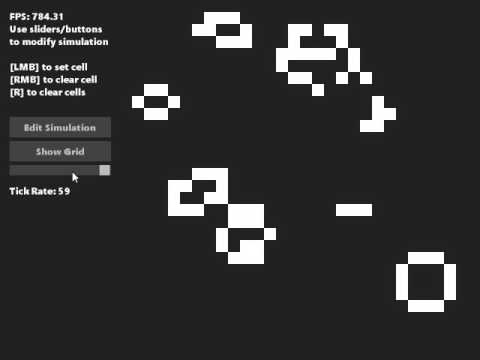
\includegraphics[width=0.8\textwidth]{img/gol_icon}
  \captionsetup{singlelinecheck=off,justification=raggedright}
\href{https://www.youtube.com/watch?v=Kzg5is1lgSk}{\caption{Video illustrations of Conway's Game of Life cellular automata in action.}}
\end{figure}
\end{frame}

\begin{frame}{Evidence for Indirect Plasticity}
\begin{figure}
    \centering
    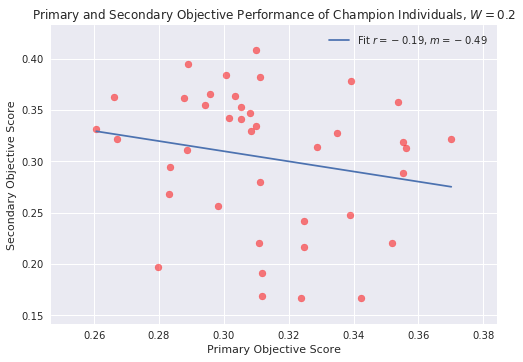
\includegraphics[width=0.8\textwidth]{img/primary_secondary_w02}
 	\captionsetup{singlelinecheck=off,justification=raggedright}
  	\caption{Primary and secondary objective performance of champion individuals evolved with primary and secondary condition/objective pair.}
    \label{fig:ev_w0}
\end{figure}
\end{frame}

\begin{frame}{Evidence for Indirect Plasticity}
\begin{figure}
    \centering
    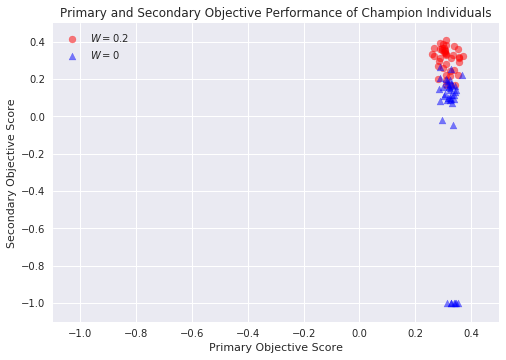
\includegraphics[width=0.8\textwidth]{img/scatter_indirect}
 	\captionsetup{singlelinecheck=off,justification=raggedright}
  	\caption{Comparison of objective performances of champions evolved with only primary condition/objective pair versus with both primary and secondary condition/objective pairs.}
    \label{fig:es_p0}
\end{figure}
\end{frame}

\begin{frame}{Evolvability as Novel Variation}
  \begin{figure}
 \centering
    \begin{subfigure}[b]{0.5\textwidth}
        \centering
    	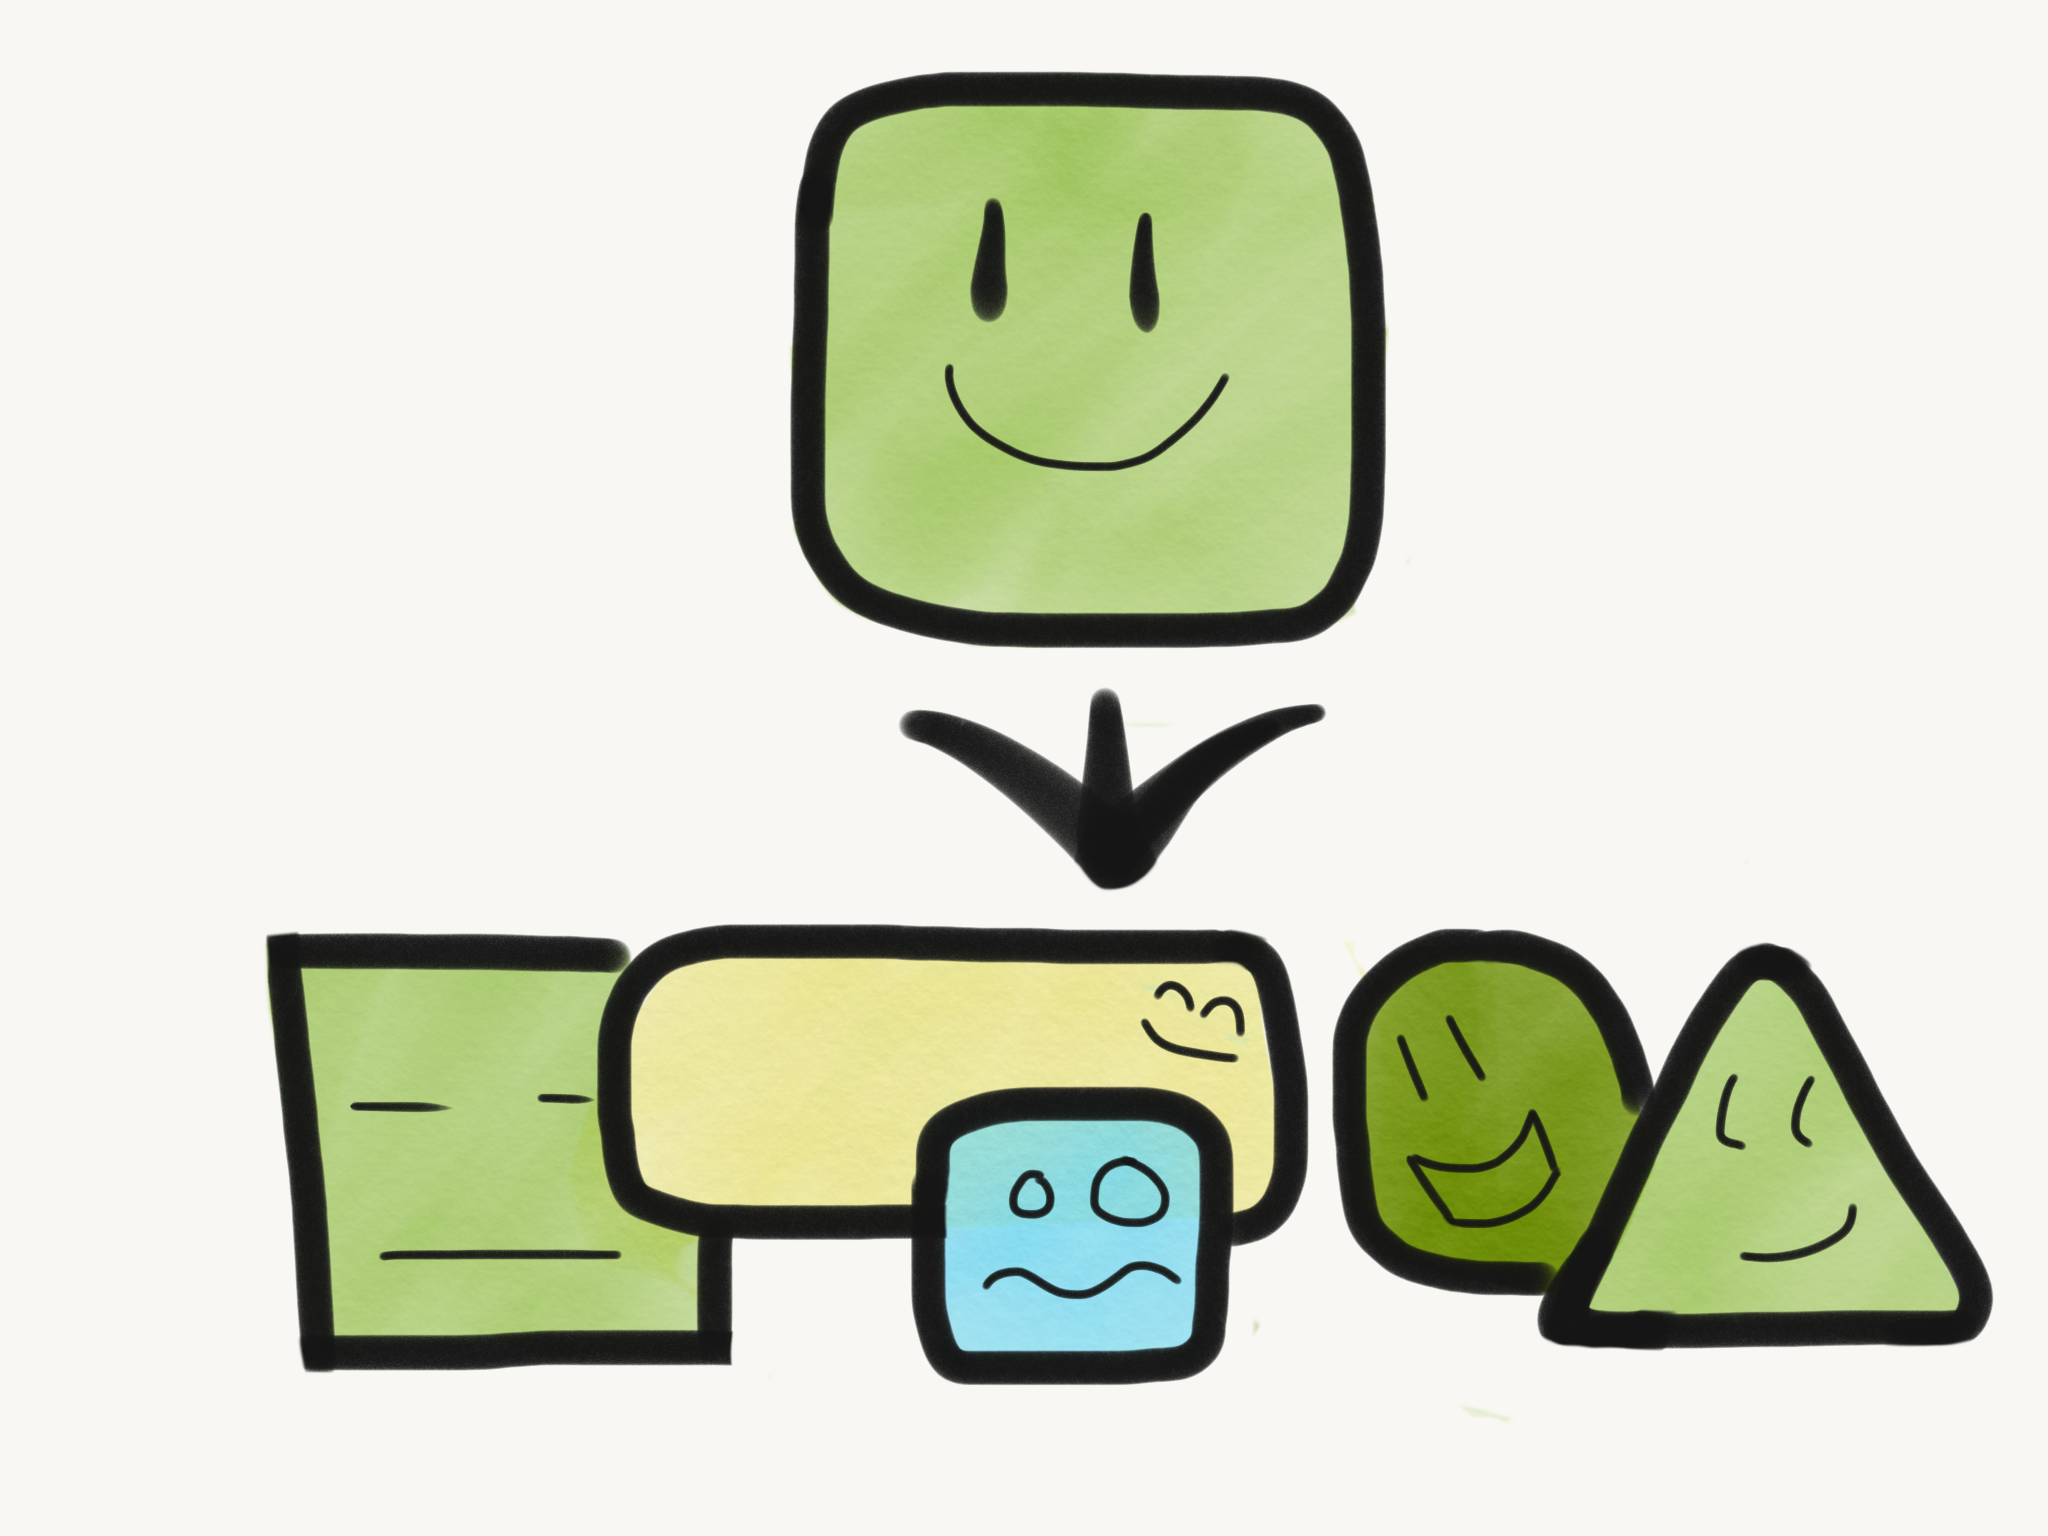
\includegraphics[width=\textwidth]{img/individual_evolvability}
        \caption{individual evolvability}
        \label{subfig:individual_evolvability}
    \end{subfigure}%
    \hfill
    \begin{subfigure}[b]{0.5\textwidth}
        \centering
        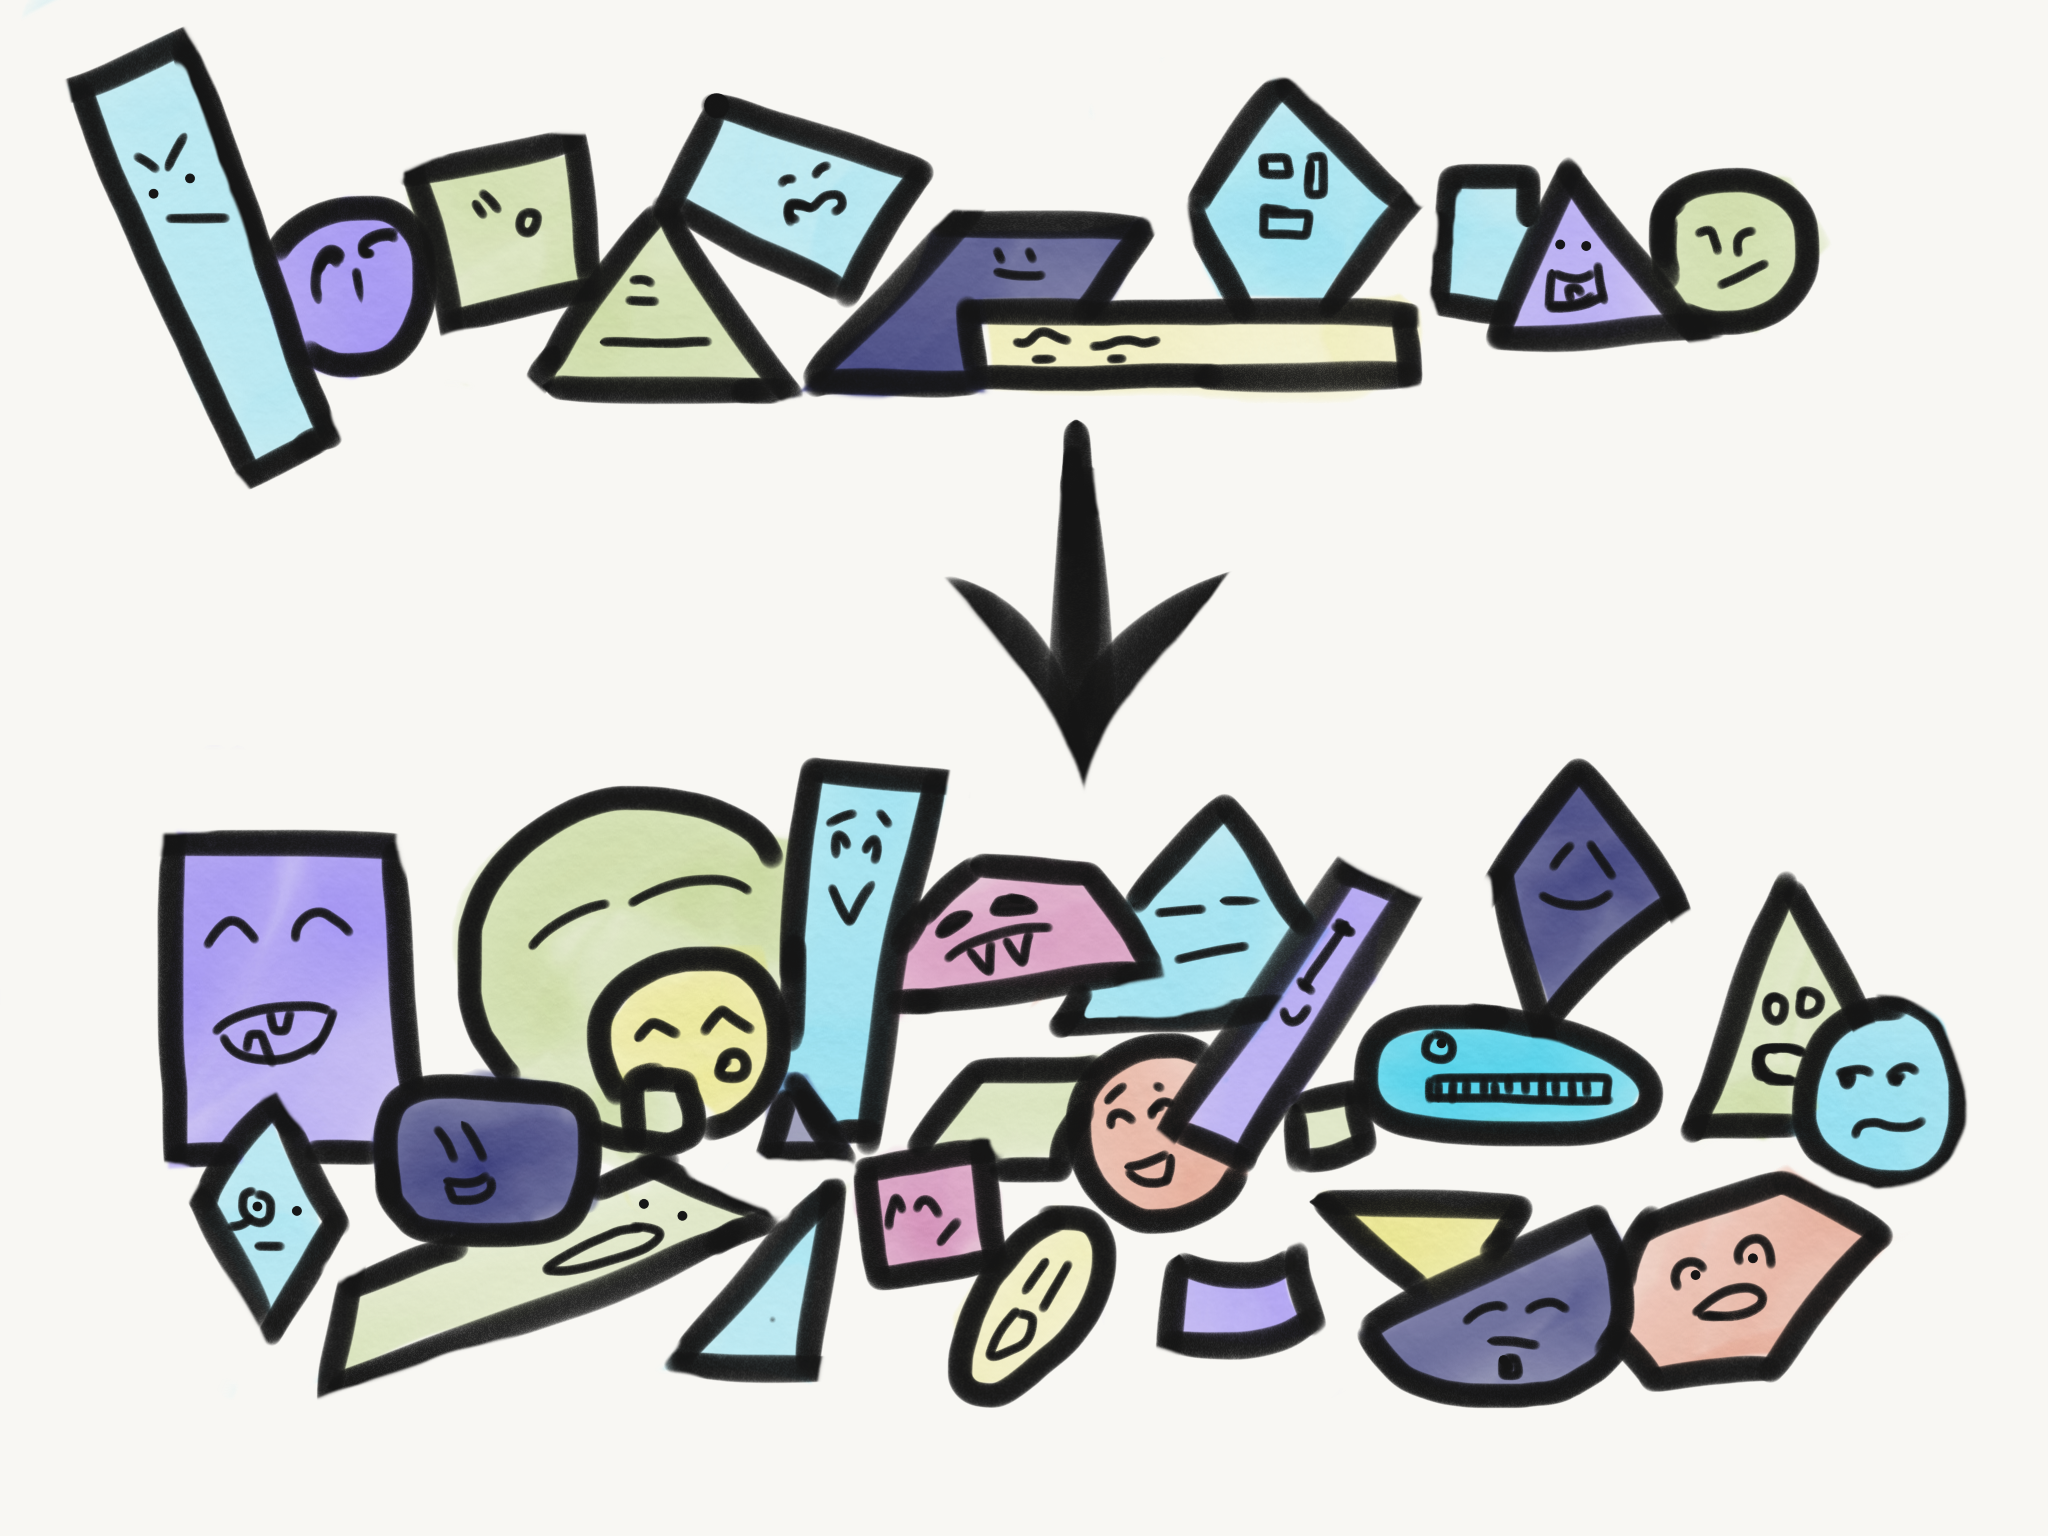
\includegraphics[width=\textwidth]{img/population_evolvability}
        \caption{population evolvability}
        \label{subfig:population_evolvability}
    \end{subfigure}
 	\captionsetup{singlelinecheck=off,justification=raggedright}
    \vspace{-4ex}
  \captionsetup{singlelinecheck=off,justification=raggedright}
  \caption{An illustration contrasting individual and population evolvability \cite{Wilder2015ReconcilingEvolvability}.}
  \label{fig:individual_vs_population_evolvability}
\end{figure}
\end{frame}

\begin{frame}{Promoting Evolvability: Fitness Niches}
	\begin{figure}
\begin{center}
\label{fig:cppn_images}
  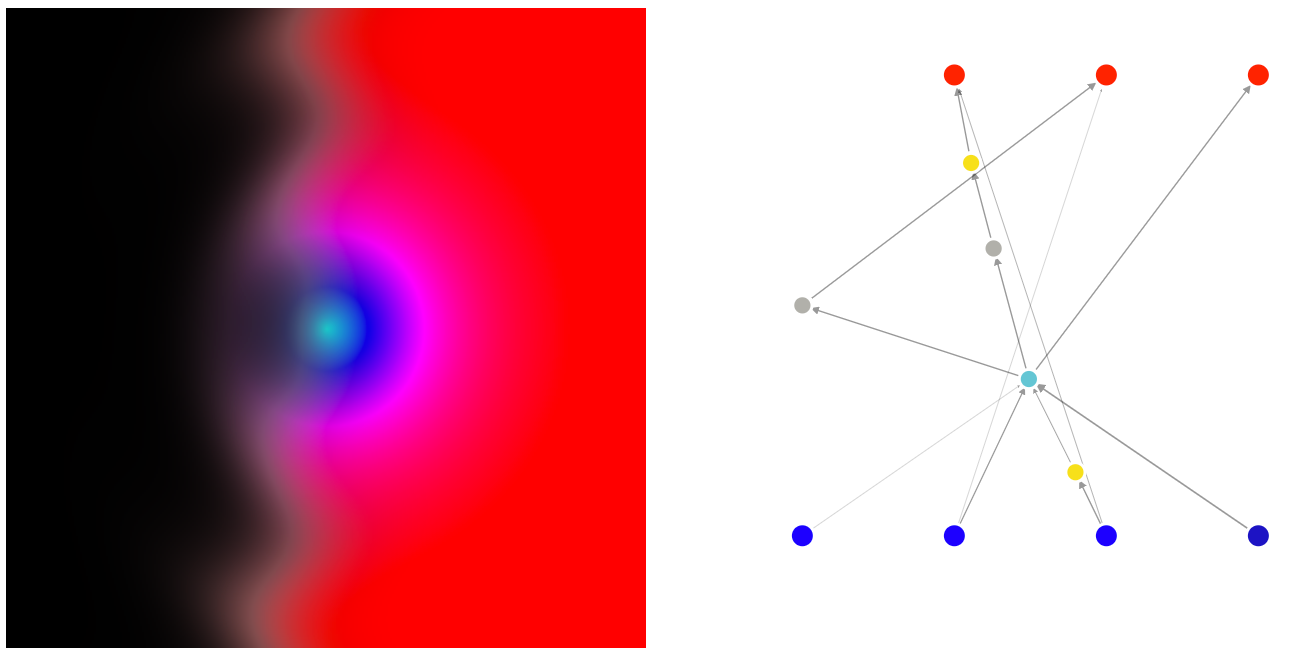
\includegraphics[width=0.4\textwidth]{img/parent} \\
  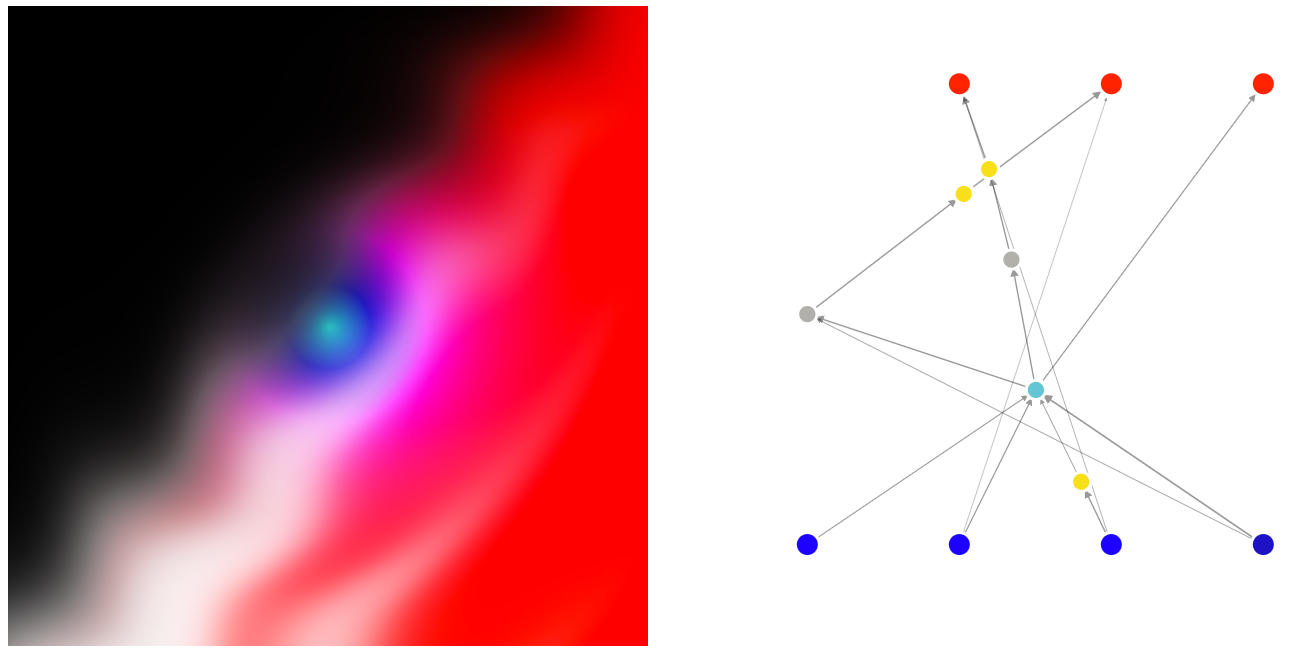
\includegraphics[width=0.4\textwidth]{img/offspring} \\
  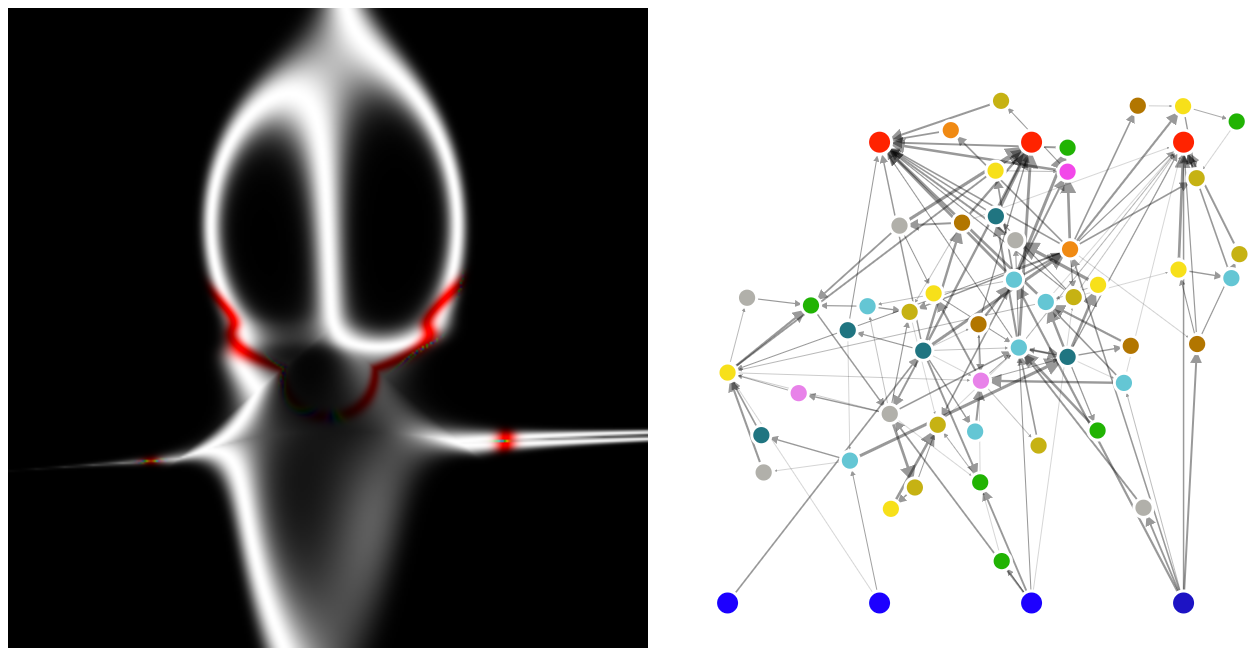
\includegraphics[width=0.4\textwidth]{img/better_goast}
  \end{center}
  \captionsetup{singlelinecheck=off,justification=raggedright}

  \caption{Illustration of compositional pattern producing networks (right) and their output images (left) generated via \cite{Ha2015Neurogram}.}
\end{figure}
\end{frame}

\begin{frame}{Promoting Evolvability: Fitness Niches}
\vfill
	\begin{figure} \label{fig:dnn}
  \begin{center}
  
\includegraphics[width=0.5\textwidth]{img/recognize} \\
  
\includegraphics[width=0.5\textwidth]{img/confused}
  \end{center}
  \captionsetup{singlelinecheck=off,justification=raggedright}

  \caption{A deep neural network (DNN) is trained to recognize a specific category of images.}
\end{figure}
    \vfill
\end{frame}

\begin{frame}{Promoting Evolvability: Fitness Niches}
\vspace{2ex}
	\begin{figure}
    \centering
  \begin{columns}
  \begin{column}{0.6\textwidth}
  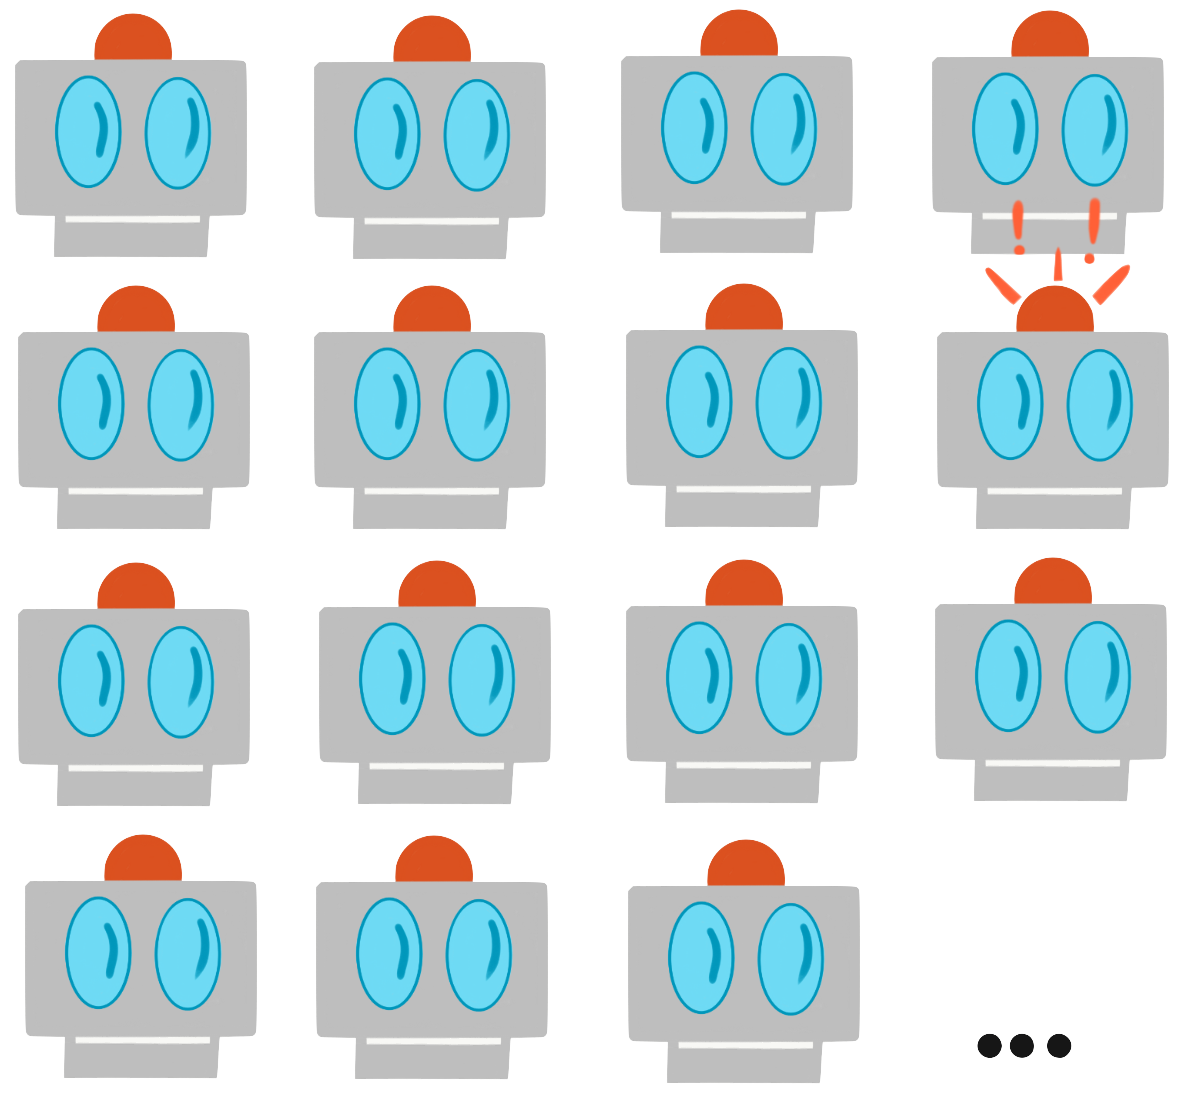
\includegraphics[width=0.9\textwidth]{img/dnn_collection}
   \end{column}
   \begin{column}{0.4\textwidth}
   
\includegraphics[width=0.9\textwidth]{img/cat}
   \end{column}
	\end{columns}
\captionsetup{singlelinecheck=off,justification=raggedright}
  	\caption{Several hundred fitness niches are defined using DNNs each trained to recognize different categories \cite{Nguyen2015InnovationLearning}.}
    \label{fig:niches}
\end{figure}
\end{frame}

\begin{frame}{Promoting Evolvability: Fitness Niches}
\vspace{2ex}	
\begin{figure}
    \centering
    \begin{columns}
    \begin{column}{0.7\textwidth}
     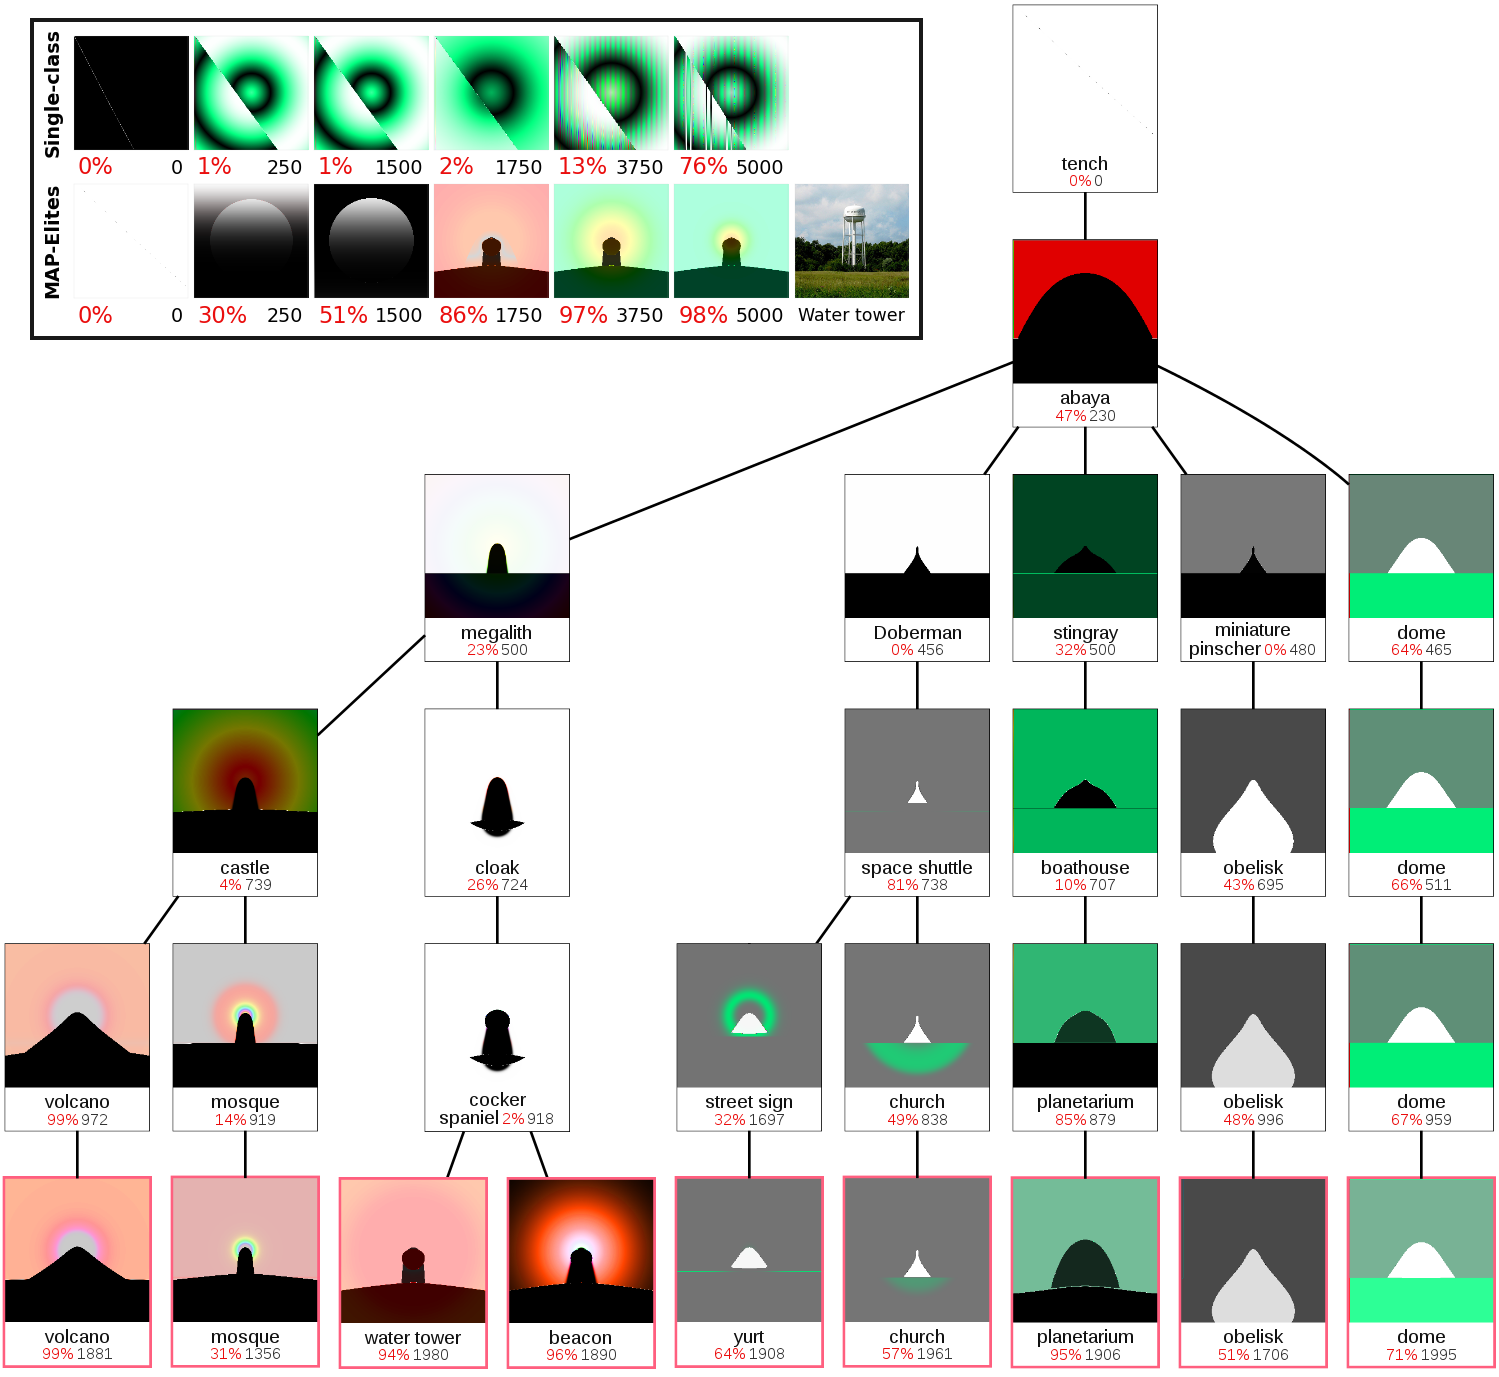
\includegraphics[width=\textwidth]{img/ie_phylogenetic_tree_combined}
    \end{column}
    \begin{column}{0.3\textwidth}
   	\captionsetup{singlelinecheck=off,justification=raggedright}
  	\caption{An illustration of goal-switching, where offspring from a parent that occupies one niche invade another \cite[Figure 9]{Nguyen2015InnovationLearning}. Individuals that promote phenotypically variable offspring are rewarded \cite{Mengistu2016EvolvabilityIt}.}
    \label{fig:goal_switching}
    \end{column}
    \end{columns}
   

\end{figure}
\end{frame}

\begin{frame}{Promoting Evolvability: Fitness Niches}
	\begin{figure}
    \centering
    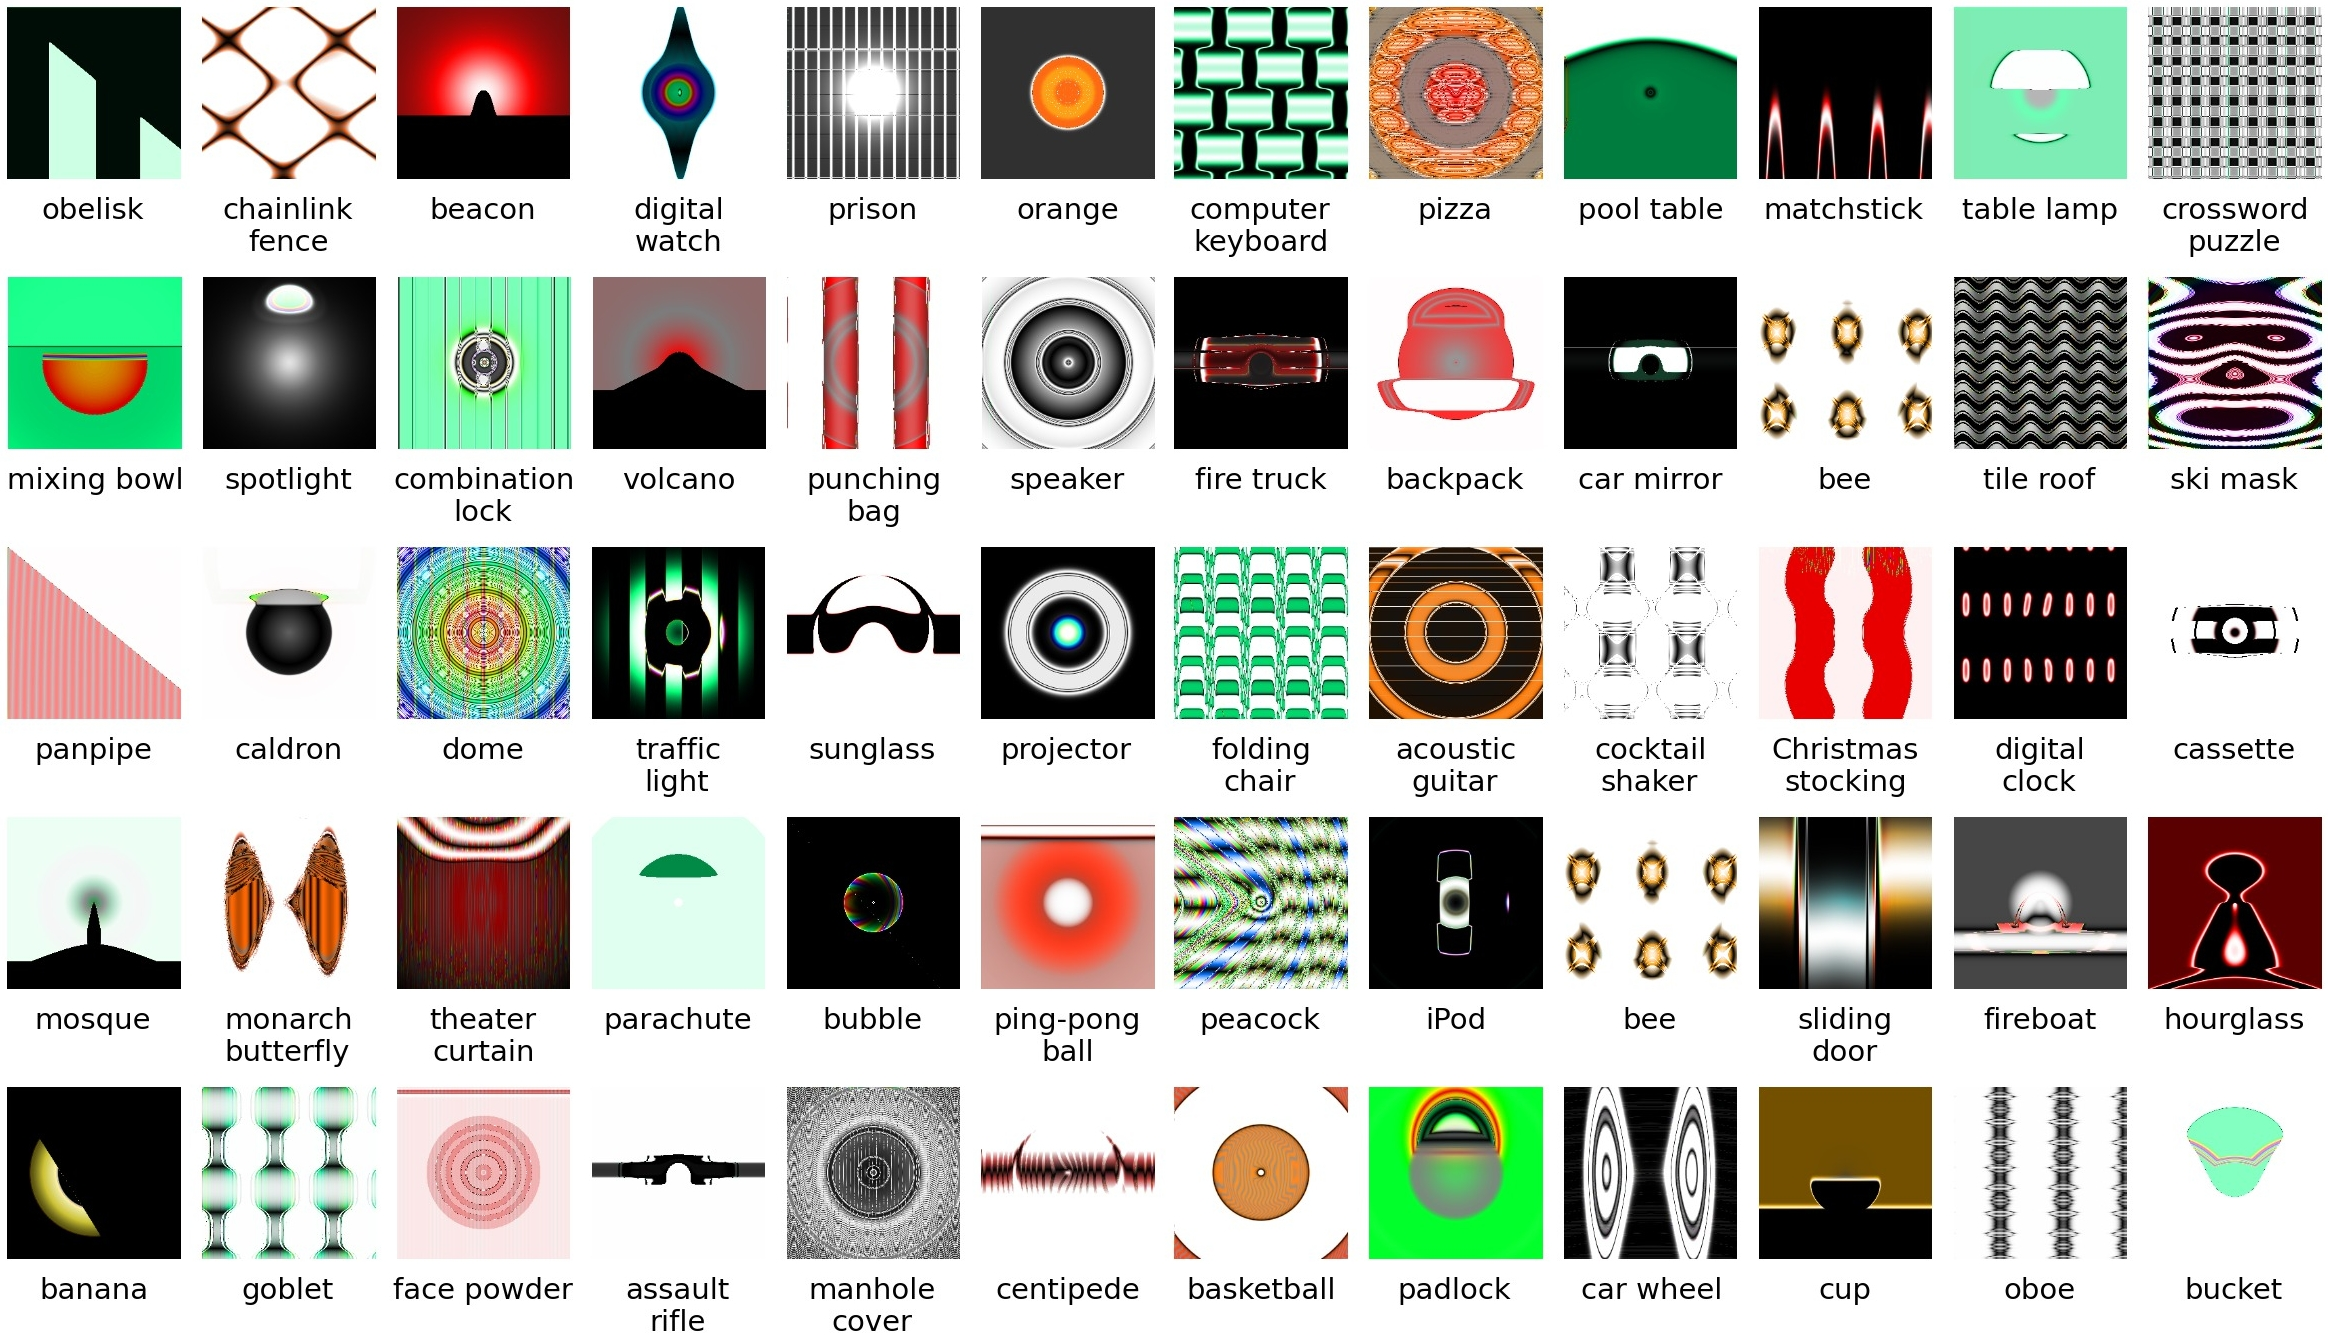
\includegraphics[width=0.9\textwidth]{img/ie_greatest_hits}
 	\captionsetup{singlelinecheck=off,justification=raggedright}
  	\caption{Selected champion individuals from a sample of environmental niches \cite[Figure 7]{Nguyen2015InnovationLearning}.}
    \label{fig:ie_results}
\end{figure}
\end{frame}


\end{document}
